\documentclass[a4paper,11pt,twoside]{report}
%%\usepackage{program}
\usepackage{amsmath}
\usepackage{ascmac}
\usepackage[dvipdfmx]{graphicx}  % for EPS and PDF 
\usepackage{url}
\usepackage{fancyvrb}
\usepackage{makeidx}
\usepackage{here}
\usepackage[dvipdfmx]{color}
\usepackage{ulem}
%\usepackage[sectionbib]{chapterbib}

%\usepackage{vruler}  %% if vertical ruler (line number) is needed
\usepackage[switch*,pagewise]{lineno}

%\usepackage[dvipdfm,bookmarkstype=toc,colorlinks=true,urlcolor=black,%
%    linkcolor=black,citecolor=black,linktocpage=true,bookmarks=false]{hyperref}
%\usepackage[dvipdfm,bookmarkstype=toc,colorlinks=true,urlcolor=black,%
%    linkcolor=black,citecolor=black,bookmarks=false]{hyperref}
\usepackage[dvipdfm,bookmarkstype=toc,urlcolor=black,%
    linkcolor=black,citecolor=black,bookmarks=false]{hyperref}

\setcounter{secnumdepth}{4}
\setcounter{totalnumber}{6}
\usepackage{fancyhdr}


\hoffset=0cm
\oddsidemargin=0cm
\evensidemargin=0cm
\textwidth=16cm
%\topmargin=-1.5cm
\topmargin=-1cm
\voffset=0cm
\textheight=24cm

\long\def\comment#1{}
\def\progenv{\baselineskip=10pt\tt\progspecial{`}\parindent=0.3cm}
\def\shellenv{\baselineskip=10pt\tt\progspecial{`}\parindent=0.3cm\nolineno}

%%\renewcommand{\topfraction}{0.85}
%%\renewcommand{\textfraction}{0.1}
%%\renewcommand{\floatpagefraction}{0.75}

\renewcommand{\topfraction}{.99}
\renewcommand{\bottomfraction}{.99}

\def\openb{{\it [}}
\def\closeb{{\it ]}}
%\def\openp{{\tt (}}
%\def\closep{{\tt )}}

\def\DAG{$^\dagger$}
\def\DDAG{$^\ddagger$}

\def\XMP{XcalableMP}
\def\OMP{OpenMP}
\def\HPF{HPF}
\def\CAF{Co-array Fortran}
\def\MPI{MPI}
\def\Fort{Fortran}
\def\C{C}
\def\XMPF{XcalableMP Fortran}
\def\XMPC{XcalableMP C}

\def\Directive#1{{\tt #1}\index{#1@{\tt #1}}\index{Directive!#1@{\tt #1}}}

%\def\Syntax#1{\index{{\tt #1}}\index{Syntax!{\tt #1}}}
\def\Syntax#1{\index{Syntax!#1@{\tt #1}}}

\def\Term#1{{#1}\index{#1}}

%\def\Example#1{\index{#1}\index{Example!{\tt #1}}}
\def\Example#1{\index{Example!#1@{\tt #1}}}

\def\Intrinsic#1{\index{#1@{\tt #1}}\index{Intrinsic and Library Procedures!#1@{\tt #1}}}

\def\NULL{{\tt NULL}}

\def\PROG#1{{\tt #1}\index{\tt #1}\index{Command!#1}}
\def\FUNC#1{{\tt #1()}\index{\tt #1}\index{Example Function!#1}}
\def\LPROG#1{{\tt #1}\index{\tt #1}\index{Linux Command!#1}}
\def\LFUNC#1{{\tt #1()}\index{\tt #1}\index{Linux Function!#1}}
\def\MFUNC#1{{\tt #1()}\index{\tt #1}\index{Myrinet/MX Function!#1}}
\def\SFUNC#1{{\tt #1()}\index{\tt #1}\index{Sample Code!#1}}
\def\STRUCT#1{{\tt #1}\index{\tt #1}\index{Struct!#1}}
\def\VAR#1{{\tt #1}\index{\tt #1}\index{Variable!#1}}
\def\ARG#1{{\tt #1}\index{\tt #1}\index{Variable!#1}}
\def\MACRO#1{{\tt #1}\index{\tt #1}\index{Macro!#1}}
\def\ERRNO#1{{\tt #1}\index{\tt #1}\index{ERRNO!#1}}
\def\SIGNAL#1{{\tt #1}\index{\tt #1}\index{Signal!#1}}
\def\FILE#1{{\tt #1}\index{\tt #1}\index{File!#1}}
\def\ENV#1{{\tt #1}\index{\tt #1}\index{Environment Variable!#1}}
\def\INDEX#1{#1\index{#1}}
\def\OPTION#1{{\tt #1}\index{Command Option!#1}}
\def\TERM#1{\underline{#1}\index{#1}}
\def\CTRL#1{{\tt $^\wedge$#1}}

\def\phrule{\vspace{0.2cm}\hrule\vspace{0.05cm}\hrule}
\def\qhrule{\vspace{0.2cm}\hrule}

\def\dhrule{\hrule\vspace{0.05cm}\hrule}

\def\bsquare{\rule[-2pt]{5pt}{10pt}}

\newcommand\gio{{\tt global\_io }}
\newcommand\mio{{\tt master\_io }}

\newcommand{\mytextcolor}[2]{\textcolor{#1}{#2}}
%\newcommand{\mytextcolor}[2]{{#2}}
\newcommand{\mycolor}[1]{\color{#1}}

\newenvironment{point}[1]{\vspace*{0.3cm}\begin{itembox}{#1}}{\end{itembox}\vspace*{0.3cm}}

\newenvironment{note}[1]{\vspace*{0.3cm}\begin{itembox}{Note on #1}}{\end{itembox}\vspace*{0.3cm}}

\newenvironment{issue}[1]{\vspace*{0.3cm}\begin{itembox}{Issues on #1}}{\end{itembox}\vspace*{0.3cm}}

\newenvironment{errors}{\vspace*{0.3cm}\begin{tabular}{ll}\multicolumn{2}{l}{\bf Return Values}\\}{\end{tabular}\vspace*{0.3cm}}

\newenvironment{mytable}[3]{\begin{table}[ht]\caption{#1}\label{#2}\vspace*{-0.3cm}\begin{center}\begin{tabular}{#3}}{\end{tabular}\end{center}\end{table}}

\newenvironment{myfigure}{\begin{figure}[ht]\begin{center}}{\end{center}\end{figure}}

\DefineVerbatimEnvironment{Fexample}{Verbatim}{numbers=left,numbersep=3pt,stepnumber=5,frame=single,label=\Fort}

\DefineVerbatimEnvironment{FexampleR}{Verbatim}{numbers=right,numbersep=3pt,stepnumber=5,frame=single,label=\Fort}

\DefineVerbatimEnvironment{Cexample}{Verbatim}{numbers=left,numbersep=3pt,stepnumber=5,frame=single,label=\C}

\DefineVerbatimEnvironment{CexampleR}{Verbatim}{numbers=right,numbersep=3pt,stepnumber=5,frame=single,label=\C}

\DefineVerbatimEnvironment{XFexample}{Verbatim}{numbers=left,numbersep=3pt,stepnumber=5,frame=single,label=\XMPF}

\DefineVerbatimEnvironment{XFexampleR}{Verbatim}{numbers=right,numbersep=3pt,stepnumber=5,frame=single,label=\XMPF}

\DefineVerbatimEnvironment{XCexample}{Verbatim}{numbers=left,numbersep=3pt,stepnumber=5,frame=single,label=\XMPC}

\DefineVerbatimEnvironment{XCexampleR}{Verbatim}{numbers=right,numbersep=3pt,stepnumber=5,frame=single,label=\XMPC}

%% End of Preemble

\title{{\Huge XcalableMP}\\
$\langle${\it ex-scalable-em-p}$\rangle$\\
Language Specification\\
%Application Program Interface\\
\vspace{2cm}
Version 1.3\\}
%DRAFT 0.7}
\author{
\Large XcalableMP Specification Working Group\\
}
\date{\vspace{4cm}\Large November, 2016}

\makeindex

\begin{document}
\maketitle

Copyright \copyright 2008-2017 {\XMP} Specification Working Group.
Permission to copy without fee all or part of this material is granted,
provided the {\XMP} Specification Working Group copyright notice and the
title of this document are displayed. Notice is given that copying
requires the explicit permission of the {\XMP} Specification Working
Group.

\clearpage
\section*{History}

\paragraph*{Version 1.2.1: Novenber, 2014.} Corrections and
clarifications to Version 1.2.

\begin{itemize}
  \item \ref{sub:align} {\tt align} Directive
  \item \ref{sub:loop_construct} {\tt loop} Directive
  \item \ref{173311_31Oct14} {\tt [C]} Declarations of Coarrays
  \item \ref{172700_31Oct14} {\tt [F] local\_alias} Directive
  \item \ref{173437_31Oct14} Array Section Notation
  \item \ref{sec:Array assignment statements in C} Array Assignment Statement
\end{itemize}

\paragraph*{Version 1.2: Novenber 20, 2013}

\paragraph*{Version 1.1: Novenber 13, 2012}

\paragraph*{Version 1.0: Novenber 14, 2011}
\cleardoublepage

\pagenumbering{roman}
\tableofcontents
\listoffigures
\listoftables
%%%%\listoftables

\chapter*{Acknowledgment}

The {\XMP} specification is designed by the {\XMP} Specification
Working Group, which consists of the following members from academia,
research laboratories, and industries.

\begin{itemize}
\setlength{\itemsep}{-1mm}
\item Tatsuya Abe        \dotfill \ RIKEN
\item Tokuro Anzaki      \dotfill \ Hitachi
\item Taisuke Boku       \dotfill \ University of Tsukuba
\item Toshio Endo        \dotfill \ TITECH
\item Yoshinari Fukui    \dotfill \ JAMSTEC
\item Yasuharu Hayashi   \dotfill \ NEC
\item Atsushi Hori       \dotfill \ RIKEN
\item Kohichiro Hotta    \dotfill \ Fujitsu
\item Hidetoshi Iwashita \dotfill \ RIKEN
\item Susumu Komae       \dotfill \ AXE
\item Atsushi Kubota     \dotfill \ Hiroshima City University
\item Jinpil Lee         \dotfill \ University of Tsukuba
\item Toshiyuki Maeda    \dotfill \ RIKEN
\item Motohiko Matsuda   \dotfill \ RIKEN
\item Yuichi Matsuo      \dotfill \ JAXA
\item Kazuo Minami       \dotfill \ RIKEN
\item Shoji Morita       \dotfill \ AXE
\item Hitoshi Murai      \dotfill \ RIKEN
\item Kengo Nakajima     \dotfill \ University of Tokyo
\item Takashi Nakamura   \dotfill \ JAXA
\item Tomotake Nakamura  \dotfill \ RIKEN
\item Mamoru Nakano      \dotfill \ CRAY
\item Masahiro Nakao     \dotfill \ RIKEN
\item Takeshi Nanri      \dotfill \ Kyusyu University
\item Kiyoshi Negishi    \dotfill \ Hitachi
\item Satoshi Ohshima    \dotfill \ University of Tokyo
\item Yasuo Okabe        \dotfill \ Kyoto University
\item Hitoshi Sakagami   \dotfill \ NIFS
\item Tomoko Sakari      \dotfill \ Fujitsu
\item Shoich Sakon       \dotfill \ NEC
\item Mitsuhisa Sato     \dotfill \ University of Tsukuba
\item Taizo Shimizu      \dotfill \ PC Cluster Consortium
\item Takenori Shimosaka \dotfill \ RIKEN
\item Yoshihisa Shizawa  \dotfill \ RIST
\item Shozo Takeoka      \dotfill \ AXE
\item Hitoshi Uehara     \dotfill \ JAMSTEC
\item Eiji Yamanaka      \dotfill \ Fujitsu
\item Masahiro Yasugi    \dotfill \ Kyushu Institute of Technology
\item Mitsuo Yokokawa    \dotfill \ Kobe University
\end{itemize}

This work was supported by ``Seamless and Highly-productive Parallel
Programming Environment for High-performance Computing'' project funded
by Ministry of Education, Culture, Sports, Science and Technology,
Japan, and is supported by PC Cluster Consortium.

\newpage
\mbox{}\newpage

\pagestyle{fancy}
\fancyhead{} % clear all header fields
\fancyhead[RE]{\leftmark}
\fancyhead[LO]{\rightmark}
\fancyhead[LE,RO]{\thepage}
\fancyfoot{} % clear all footer fields
\renewcommand{\headrulewidth}{0pt}
\renewcommand{\footrulewidth}{0pt}

%\setvruler[][][][3][0][1.2\textwidth]
\pagewiselinenumbers

\chapter{Introduction}
\pagenumbering{arabic}
\setcounter{page}{1}

This document defines the {\XMP} specification, which is a
directive-based language extension of {\Fort} and {\C} for scalable and
performance-aware parallel programming.
%
The specification includes a collection of compiler directives and
intrinsic and library procedures, and provides a model of parallel
programming for distributed memory multiprocessor systems.

%This document specifies a collection of compiler directives and runtime
%library routines that can be used to write distributed-memory parallel
%programs in {\C} and {\Fort}.These compiler directives define the
%specifications of the {\XMP} Application 
%Program Interface ({\XMP} API). These specifications provide a
%model of parallel programming for distributed memory multiprocessor
%systems. The directives extend the {\C} and {\Fort} base languages to
%describe distributed memory parallel programs.

\section{Features of {\XMP}}

The features of {\XMP} are summarized as follows:

\begin{itemize}

 \item {\XMP} supports typical parallelization based on the
       data-parallel paradigm and work mapping under the ``global-view''
       programming model, and it enables the parallelization of the
       original sequential code using minimal modification with simple
       directives such as {\OMP} \cite{omp}. Many ideas on ``global-view''
       programming are inherited from High Performance Fortran ({\HPF})
       \cite{hpf}.

 \item The important design principle of {\XMP} is
       ``performance-awareness.'' All actions related to communication
       and synchronization are taken by directives (and coarray features),
       which is different from automatic parallelizing compilers. The
       user should be aware of the effect of the {\XMP} directives in
       the execution model for distributed-memory architecture.

 \item {\XMP} also includes features from Partitioned Global Address
       Space (PGAS) languages, such as coarray of the {\Fort} 2008
       standard, for ``local-view'' programming.

 \item An extension of existing base languages with directives is useful
       to reduce code-rewriting and education costs. The {\XMP} language
       specification is defined as an extension to the {\Fort} and {\C}
       base languages.

 \item For flexibility and extensibility, the execution model enables us
       to combine {\XMP} with explicit Message Passing Interface ({\MPI})
       \cite{mpi} coding for more complicated and tuned parallel codes
       and libraries.

 \item For multi-core and SMP clusters, {\OMP} directives can be
       combined into {\XMP} for thread programming inside each node as a
       hybrid programming model.

% \item {\bf Language extensions} for familiar languages, such as {\C}
%       and Fortran, which can reduce code-rewriting and educational
%       costs.
%
% \item {\XMP} supports typical parallelization based on the {\bf data
%       parallel paradigm} and work sharing under {\it global view} and
%       enables parallelization of the original sequential code with
%       minimal modification using simple {\bf directives}, such as
%       {\OMP}.
%
% \item {\XMP} also includes a CAF-like Partitioned Global Address Space
%       (PGAS) feature as {\it local-view} programming.
%
% \item {\bf Explicit communication and synchronization}. All actions are
%       taken by directives for being ``easy-to-understand'' for
%       performance-aware programming
%
% \item For flexibility and extensibility, the execution model allows
%       {\bf combination with explicit {\MPI} coding} for more
%       complicated and tuned parallel codes and libraries.
%
% \item For multi-core and SMP clusters, {\bf {\OMP} directives can be
%       combined} into {\XMP} for thread programming inside each node as
%       a hybrid programming model.

\end{itemize}

{\XMP} is being designed based on experiences gained during the
development of HPF, HPF/JA \cite{hpfja}, Fujitsu XPF (VPP
FORTRAN) \cite{XPF,VPPFORTRAN}, and OpenMPD \cite{OpenMPD}.

\section{Scope}

The {\XMP} specification covers only user-directed parallelization,
where the user explicitly specifies the behavior of the compiler and
the runtime system in order to execute the program in parallel in a
distributed-memory system.
%
{\XMP}-compliant implementations are not required to automatically
distribute data, detect parallelism, parallelize loops, or generate
communications and synchronizations.

%The {\XMP} is defined by following items:
%
%\begin{itemize}
%\item A set of directives
%\item Minimum language extension on base languages ({\C} and {\Fort})
%\item Runtime libraries
%\item Environment Variables
%\end{itemize}

\section{Organization of this Document}

The remainder of this document is structured as follows:

\begin{itemize}
 \item Chapter 2: Overview of the {\XMP} Model and Language
 \item Chapter 3: Base Language Extensions in {\XMPC}
 \item Chapter 4: Directives 
 \item Chapter 5: Support for Local-view Programming
 \item Chapter 6: Procedure Interface
 \item Chapter 7: Intrinsic and Library Procedures
 \item Chapter 8: OpenMP in XcalableMP Programs
\end{itemize}
%
In addition, the following appendices are included in this document as
proposals.
%
\begin{itemize}
 \item Appendix A: Programming Interface for MPI
% \item Appendix B: Directive for Thread Parallelism
 \item Appendix B: Interface to Numerical Libraries
 \item Appendix C: Memory-layout Model
 \item Appendix D: XcalableMP I/O
 \item Appendix E: Memory Consistency Model
 \item Appendix F: DRAFT: Tasklet of upcoming XcalableMP 2.0
\end{itemize}

\section{Changes to Version 1.4 from Version 1.3}
\begin{itemize}
  \item Combined directives in XcalableMP C are allowed.
%  \item Add an appendix about the coarray features.
  \item Add an appendix about the tasklet featues of upcoming {\XMP} 2.0.
\end{itemize}

\section{Changes to Version 1.3 from Version 1.2.1}
\begin{itemize}
  \item In XcalableMP C, a square bracket is available in {\it nodes-decl}, {\it nodes-ref}, 
  {\it template-ref}, and {\it template-decl}.
  \item Add the {\tt orthogonal} clause to the {\tt reflect} directive in Section \ref{sub:reflect}.
  \item Add {\tt xmpc\_all\_node\_num()} in Section \ref{sub:xmpcallnodenum}.
  \item Add {\tt xmpc\_node\_num()} in Section \ref{sub:xmpcnodenum}.
  \item Add {\tt xmpc\_this\_image()} in Section \ref{sub:xmpcthisimage}.
  \item Add {\tt xmp\_num\_images()} in Section \ref{sub:xmpnumimages}.
  \item Modify {\tt xmp\_array\_gtol()} in Section \ref{subsec:xmparraygtol}.
  \item Change {\tt xmp\_array\_lsize()} not to include shadow object in Section \ref{subsec:xmparraylsize}.
  \item Create {\tt xmp\_array\_lda()} from {\tt
		xmp\_array\_lead\_dim()} in Section \ref{subsec:xmparraylda}.

  \item In XcalableMP C, the dynamic allocataion of multi-dimensional global
		data is allowed.
  \item A restriction on the {\tt align} directive is added.
  \item The {\tt expand} and {\tt margin} clauses of the {\tt loop}
		construct are added.
  \item The meaning of a reduction-kind ``{\tt -}'' in the {\tt
		reduction} clause of the {\tt loop} construct is changed.
  \item The treatment for {\it async-id} not associated with any asynchronous
		communication is specified.
  \item The {\tt reduce\_shadow} construct is added.
  \item The description of the {\tt local\_alias} directive is modified.
  \item The {\tt xmp\_exit} library function is added.
  \item The specifications of {\tt xmp\_scatter}, {\tt xmp\_pack}, and
		{\tt xmp\_unpack} are modified.
  \item The memory consistency model of {\XMP} is discussed in the appendix.
\end{itemize}

\section{Changes to Version 1.1 from Version 1.2}

\begin{itemize}
 % \item The concept of the node array and the node set is reorganized.
 % \item Mapping inquiry procedures are expanded and moved from the
 %       appendix to the core specification.
 % \item The specification on coarrays is improved significantly and some
 %       image control directives in XMP/C are defined.
 % \item The appendix on a directive for thread parallelism is deleted.
 % \item The proposal on XcalableMP I/O is changed slightly and adopted.
 % \item etc.
 % \item The concept of built-in function is introduced into {\XMPC}.
 % \item The semantics of array intrinsic functions of the base language
 %       appearing in {\XMPF} programs is defined.
 % \item Built-in elemental functions for {\XMPF} are defined.
 % \item Intrinsic/built-in transformational procedures are defined.
 % \item The rule for mixing {\XMP} and OpenMP in a program is defined.
  \item The position of {\tt align} directives for dummy arguments
		in {\XMPC} is specified.
  \item It is specified that aligned arrays cannot be initialized.
  \item The interpretation of a {\tt reduction} clause of the {\tt loop}
		directive is corrected.
  \item The syntax for declaring coarrays is changed.
  \item An assumed-shape array can be the target of the {\tt
		local\_alias} directive.
  \item The syntax and the semantics of the array section notation in
		{\XMPC} is modified.
  \item The syntax of the array assignment statement in {\XMPC} is
		extended.
\end{itemize}


\cleardoublepage

\chapter{Overview of the {\XMP} Model and Language}
\label{chap: overview}

\section{Hardware Model}

The target of {\XMP} is distributed-memory multicomputers (Figure
\ref{fig1}). Each computation node, which may contain several cores, has
its own local memory (shared by the cores, if any), and is connected
with the others via an interconnection network.
%
Each node can access its local memory directly and remote memory (the
memory of another node) indirectly (i.e., through inter-node 
communication). However, it is assumed that accessing remote memory is 
much slower than accessing local memory.

\begin{myfigure}
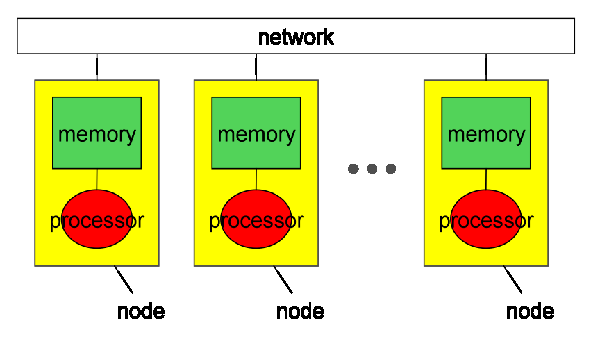
\includegraphics[width=12cm]{figs/Fig1.eps}
  \caption{Hardware model.}\label{fig1}
\end{myfigure}

\section{Execution Model}

An {\XMP} program execution is based on the Single Program Multiple Data
(SPMD) model, where each node starts execution from the same main
routine, and continues to execute the same code independently
(i.e., asynchronously), which is referred to as the {\it \Term{replicated
execution}}, until it encounters an {\XMP} construct.

%The basic execution model of {\XMP} is a Single Program Multiple Data
%(SPMD) model on distributed memory. In each node, a program starts from
%the same main routine.
%
%Unless the nodes encounter some {\XMP} directives, they executes the same
%code locally (i.e. asynchronously), which is referred to as
%{\it \Term{duplicate execution}}.

%An {\XMP} program begins as a single thread of
%execution in each node. 

%In this case, the
%program performs duplicate execution of the same program on local memory
%in each node.

%{\OMP} API can be used in order to make use of multicores in a node. In
%this specification, we define actions only when {\XMP} directives are
%executed one thread at a time.

A set of nodes that executes a procedure, statement, loop,
a block, etc. is referred to as its {\it \Term{executing node set}}, and is
determined by the innermost {\tt task}, {\tt loop}, or {\tt array}
directive surrounding it dynamically, or at runtime.
%
The {\it \Term{current executing node set}} is an executing node set of
the current context, which is managed by the {\XMP} runtime system on
each node.

%The initial ``current executing node set'' (or the {\it \Term{entire
%node set}}) at the beginning of the program execution is the set of all
%available nodes, which can be specified in an implementation-defined
%way (e.g. through a command-line option).

The current executing node set at the beginning of the program
execution, or {\it \Term{entire node set}}, is a node set that
contains all the available nodes, which can be specified in an 
implementation-defined way (e.g., through a command-line option).
%
%The entire node array is the node array if specified explicitly by the
%{\tt nodes} directive or an implicit one-dimensional node array if not.
%}

When a node encounters at runtime either a {\tt loop}, {\tt array}, or
{\tt task} construct, and is contained by the node set specified by the
{\tt on} clause of the directive, it updates the current executing node
set with the specified one and executes the body of the construct, after
which it resumes the last executing node set and proceeds to execute the
subsequent statements.

In particular, when a node in the current executing node set encounters a
{\tt loop} or an {\tt array} construct, it executes the loop or the array
assignment in parallel with other nodes, so that each iteration of the
loop or element of the assignment is independently executed by the node
in which a specified data element resides.

When a node encounters a synchronization or a communication directive,
synchronization or communication occurs between it and other nodes.
%
That is, such {\it \Term{global constructs}} are performed collectively
by the current executing nodes.
%
Note that neither synchronization nor communication occurs unless these
constructs are being specified.


\section{Data Model}

%By default, data declared in the program are allocated in each node and
%are referenced locally by threads executed in the node. 

There are two classes of data in {\XMP}: {\it \Term{global data}} and
{\it \Term{local data}}. Data declared in an {\XMP} program are local by
default.

Global data are distributed onto the executing node set by
the {\tt align} directive (see section \ref{sub:align}). Each fragment
of distributed global data is allocated in the local memory of a node in the
executing node set.
%
%Note that the ``address'' of a global data object is defined as that of its
%local section in each node and the results of any operations on such
%address are undefined.
%
%In contrast to a local-view programming model, a global-view programming
%model is a model in which programmers express their algorithm and data
%structure in their entirety, mapping them to the node set. The
%programmers describe the data distribution and the work mapping in order
%to express how to distribute data and share the workload among
%nodes. The variables in the global-view programming model appear as a
%shared memory spanning the nodes.

Local data comprises all data that are not global. They are replicated
within the local memory of each of the executing nodes.

%{\XMP} supports two models of data viewing: the global-view programming
%model and the local-view programming model. In the local-view
%programming model, accesses to data in remote nodes are performed
%explicitly by language extension for get/put operations on remote nodes
%with the node number of the target nodes, while reference to local data
%is executed implicitly.

A node can access directly only local data and sections of global data
that reside in its local memory.
%
To access data in remote memory, explicit communication must be
specified in ways such as global communication constructs and
coarray assignments.

%\underline{Description on memory layout to be added.}

In particular, in {\XMPF}, for common blocks that include any global
variables, it is implementation-defined what storage sequences they
occupy and how storage association is defined between two of them.

\section{Global-view Programming Model}

The global-view programming model is useful when, starting from a
sequential version of a program, the programmer parallelizes it in
data-parallel style by adding directives with minimum modification.
%
In the global-view programming model, the programmer describes the
distribution of data among nodes using the data distribution
directives.
%
The {\tt loop} construct assigns each iteration of a loop to the node
at which the computed data is located. 
%
The global-view communication directives are used to synchronize nodes,
maintain the consistency of shadow areas, and move sections of 
distributed data globally.
%
Note that the programmer must specify explicitly communications to make
all data references in the program local, and this is done using
appropriate directives.
%Note that the programmer must perform all computations that require data
%reference locally by any appropriate directives.

In many cases, the {\XMP} program according to the global-view
programming model is based on a sequential program, and it can produce
the same results, regardless of the number of nodes (Figure
\ref{fig2}).
%The global view provides a 
%programming model in which computation and data are distributed onto
%computation nodes.

There are three groups of directives for the global-view programming
model. Because these directives are ignored as a comment by the
compilers of base languages ({\Fort} and {\C}), an {\XMP} program can be
compiled by them to ensure that they run properly.

%an  {\XMP} program derived from a sequential program can preserve the
%integrity of the original program when the program is run sequentially. 

\subsubsection*{Data Mapping}

Specifies the data distribution and mapping to nodes (partially
inherited from HPF).

\subsubsection*{Work Mapping (Parallelization)}

Assigns a work to a node set. The {\tt loop} construct maps each
iteration of a loop to nodes owning a specific data elements. The {\tt
task} construct defines a set amount of work as a {\it \Term{task}}, and
assigns it to a specific node set.

\subsubsection*{Communication and Synchronization}

Specifies how to communicate and synchronize with the other compute
nodes. In {\XMP}, inter-node communication must be explicitly specified
by the programmer. The compiler guarantees that no communication occurs
unless it is explicitly specified by the programmer.

\begin{myfigure}
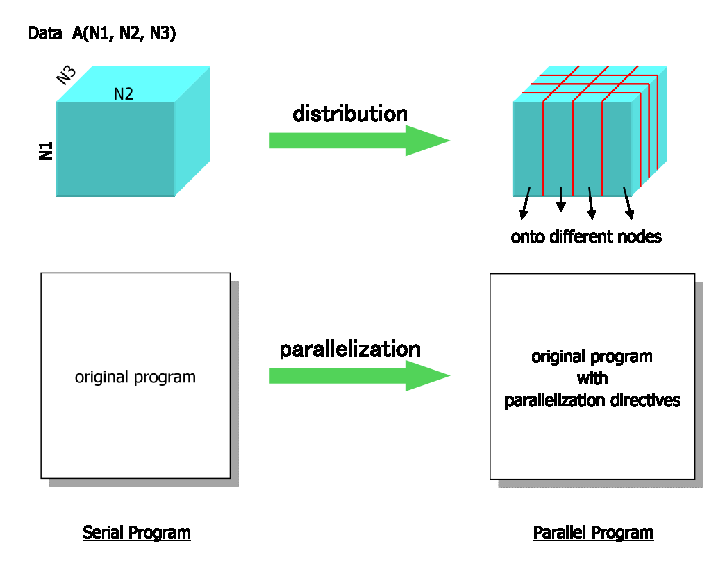
\includegraphics[width=12cm]{figs/Fig2.eps}
  \caption{Parallelization using the global-view programming model.}
\label{fig2}
\end{myfigure}

\section{Local-view Programming Model}

The local-view programming model is suitable for programs that
explicitly describe an algorithm and a remote data reference that are to
be executed by each node (Figure \ref{fig3}).
%Since MPI is based on the local-view model, the local-view programming
%model of {\XMP} has high interoperability with MPI.

For the local-view programming model, some language extensions and 
directives are provided. The coarray notation, which is imported from
{\Fort} 2008,
is one such extension, and can be used to specify which replica of a
local data is to be accessed. For example, the expression of {\tt
A(i)[N]} is used to access an array element of {\tt A(i)} located on the
node {\tt N}.
%
If the access is a reference, then a one-sided communication to get the
value from the remote memory (i.e., the {\it get} operation) is issued
by the executing node.
If the access is a definition, then a one-sided communication to put a
value to the remote memory (i.e., the {\it put} operation) is issued by
the executing node.

\begin{myfigure}
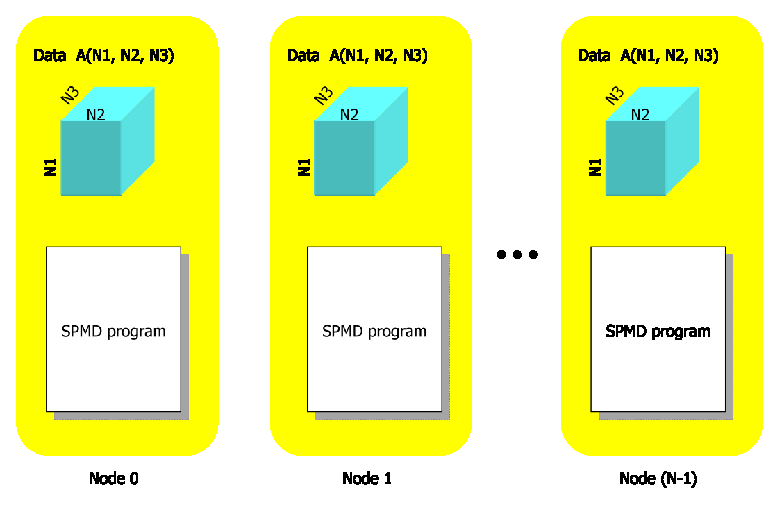
\includegraphics[width=12cm]{figs/Fig3.eps}
  \caption{Local-view programming model.}
\label{fig3}
\end{myfigure}

\section{Interactions between Global View and Local View}

In the global view, nodes are used to distribute data and works. In the
local view, nodes are used to address data in the coarray notation.
%
In application programs,
programmers should choose an appropriate data model according to the
structure of the program. Figure \ref{fig4} illustrates the global view
and the local view of data.

Data may have both a global view and a local view, and can be accessed
from either. {\XMP} provides some directives to give the local name
(alias) to the global data declared in the global-view programming model
to enable them to also be accessed in the local-view programming
model. This feature is useful to optimize a certain part of the program
by using explicit remote data access in the local-view programming
model.

\begin{myfigure}
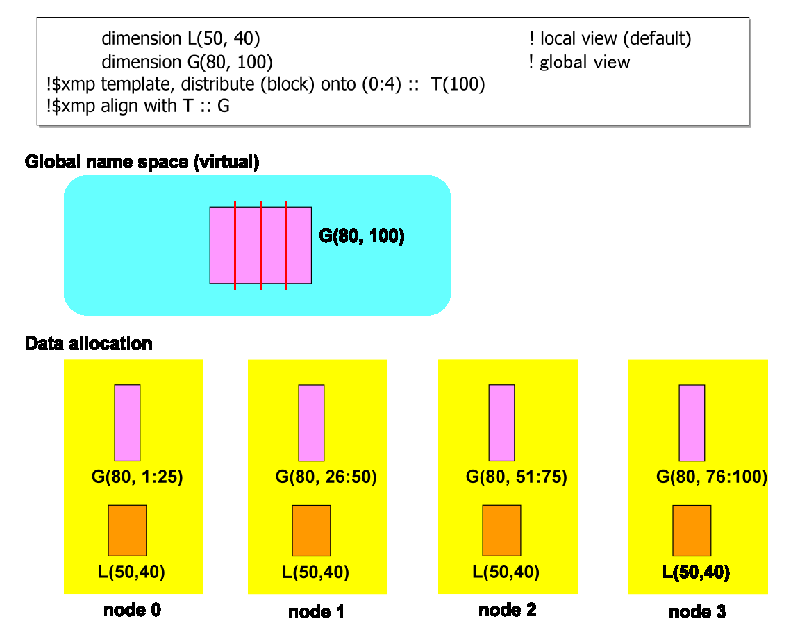
\includegraphics[width=12cm]{figs/Fig4.eps}
  \caption{Global view and local view.}
\label{fig4}
\end{myfigure}

\section{Base Languages}

The XcalableMP language specification is defined based on Fortran
and C as the base languages. More specifically, the base language of XcalableMP 
Fortran is Fortran 90 or later, and that of XcalableMP C is ISO C90
(ANSI C89) or later.

%\section{Execution model and task}
%
%
%In {\XMP}, a program begins as a single thread
%of execution in each node. The set of nodes when starting a program is
%referred to as the entire node set.
%
%A task is a specific instance of executable
%code and its data environment executed in a set of nodes. A task when
%starting a program in the entire node set is called an initial task. The
%initial task can generate a subtask, which is executed on a subset of the
%nodes by the {\tt task} construct. A set of nodes executing the same task is
%referred to as the set of executing nodes. If no {\tt task} construct is encountered, then a
%program is executed as a single task, and its executing nodes are the entire node set.
%
%If no directives are encountered, then a program is executed
%locally. When the same codes are executed, almost the same computation is
%performed in each node, which is referred to as duplicate execution. When the threads
%encounter a {\tt loop} construct or an {\tt array} construct, the specified
%loop is executed in parallel, so that each iteration is assigned to the
%node where the specified data element is located. 
%
%A new task is generated by
%the {\tt task} construct. A code in the {\tt task} construct is executed
%as a subtask executed in a specified node set. When a subroutine is
%called in the context of the task, the subroutine is executed on its
%executing nodes. 
%
%For synchronization and communication between nodes, a set of
%directives is provided. In the local-view programming model, coarray
%features are adopted for remote data reference. Note 
%that all synchronization and communication are specified explicitly by directives, and without such directives, no communications are
%executed implicitly by the compiler.

\newcommand{\namelistlabel}[1]{\mbox{#1}\hfil}
\newenvironment{namelist}[1]{%
\begin{list}{}
       {\let\makelabel\namelistlabel
        \settowidth{\labelwidth}{#1}
        \setlength{\leftmargin}{1.3\labelwidth}
}
}{%
\end{list}}

\newcommand{\gitem}[1]{\item[{\parbox[b]{3.3cm}{\raggedleft \bf \Term{#1}}}]}


\section{Glossary}

\subsection{Language Terminology}

\begin{namelist}{entire node setxxxx}

\gitem{base language}

 A programming language that serves as the foundation of the {\XMP}
 specification.

\gitem{base program}

 A program written in a base language.

\gitem{structured block}

 For C, an executable statement, possibly compound, with a single entry
 at the top and a single exit at the bottom, or an OpenMP construct.
 For Fortran, a block of executable statements with a single entry at
 the top and a single exit at the bottom, or an OpenMP construct.

\gitem{procedure}

 A generic term used to refer to ``procedure'' (including subroutine and
 function) in Fortran and ``function'' in C.

\gitem{directive}

 In C, a {\tt \#pragma}, and in Fortran, a comment, that specifies
 {\XMP} program behavior.

\gitem{declarative directive}

 An {\XMP} directive that may only be placed in a declarative context. A
 declarative directive has no associated executable user code, but
 instead has one or more associated user declarations.

\gitem{executable directive}

 An {\XMP} directive that is not declarative; it may be placed in an
 executable context.

\gitem{construct}

 An {\XMP} executable directive (and for Fortran, the paired end
 directive, if any) and the associated statement, loop or structured
 block, if any.

%, not
%including the code in any called routines; i.e., the lexical extent of an
%executable directive.

\gitem{global construct}

 A construct that is executed collectively and synchronously by all
 nodes in the executing node set. Global constructs are further
 classified into two groups of {\it global communication constructs},
 such as {\tt gmove}, {\tt barrier}, etc., which specify communication
 or synchronization, and {\it work mapping constructs}, such as {\tt
 loop}, {\tt array} and {\tt tasks}, which specify parallelization of
 loops, array assignments or a set of tasks.

\gitem{template}

 A dummy array that represents an index space to be distributed onto a
 node set, which serves as the ``template'' of parallelization in
 {\XMP} and can be considered to abstract, for example, a set of grid
 points in the grid method or particles in the particle method.
%
 A template is used in an {\XMP} program to specify the data and the
 work mapping.

%A dummy array used to express an index space associated
%with an array. Template is also used to describe the iteration space of
%a loop. A template has a name, a dimension, and an upper and  lower
%bound for each dimension as attributes.

\gitem{data mapping}

 Allocating elements of an array to nodes in a node set by specifying
 with the {\tt align} directive that the array is aligned with a
 distributed template.

%\gitem{work}

\gitem{work mapping}

 Assigning iterations of a loop, elements of an array assignment, or
 tasks in a task set to nodes in a node set by specifying with one of
 the work mapping constructs that the loop, the assignment, or the set
 is aligned with a template or distributed onto a node array.

%\subsection*{\Term{data mapping}}
%The combination of the alignment and
%distribution attributes used to describe how a data object is
%allocated to nodes.
%
%\subsection*{\Term{work mapping}}
%Assignment of iterations to nodes in
%a parallel loop and tasks to nodes.

\gitem{global}

 A data or a work is {\it global} if and only if there is only one
 instance of it shared by all nodes in the executing node set.

\gitem{local}

 A data or a work is {\it local} if and only if there is a replicated
 instance of it in each node in the executing node set.

\gitem{global-view model}

 A model of programming or parallelization on which parallel programs
 are written by specifying how to map global data and works onto nodes.

\gitem{local-view model}

 A model of programming or parallelization on which parallel programs
 are written by specifying how each node owns local data and does local
 works.

%Execution of a program has side-effects only on the data in the node. In
%this case, no communication with other nodes occurs .

%\subsection*{\Term{non-local}}
%
%Execution of a program requires
%communication with other nodes and has side-effects with respect to other
%nodes. 

\end{namelist}


\subsection{Node Terminology}

\begin{namelist}{entire node setxxxx}

\gitem{phisical node}

 A computing component of a distributed-memory multicomputer, which has
 its own main memory and is connected with each other via an
 interconnect. A node may contain multiple cores sharing the main
 memory.

%In a distributed memory system, a computation node, which may have
%several cores sharing main memory, has its own local memory. Each node
%is connected through a network. An \XMP program begins as a single
%thread of execution in each node.

\gitem{(logical) node}

 An execution entity managed and assigned to a phisical node at runtime
 by the {\XMP} runtime system, which has its own memory and can
 communicate with other nodes. A node can execute one or more threads
 concurrently.

\gitem{node set}

 A set of nodes.

\gitem{entire node set}

 A node set that contains all of the nodes participating in the
 execution of an XcalbleMP program.

\gitem{(current) executing node set}

 A node set that contains all of the nodes participating in the
 execution of a procedure, a statement, a construct, etc. of an
 XcalableMP program is called its executing node set. The current
 executing node set can be modified by the {\tt task}, {\tt array}, or
 {\tt loop} direcitives. Note that the executing node set of the main
 routine is the entire node set.

\gitem{node array}

 An entity of the same form as a Fortran array that represents a node
 set in XcalableMP programs. Each element of a node array represents a
 node in the corresponding node set. A node array is declared by the
 {\tt nodes} directive.

\gitem{parent node set}

 The parent node set of a node set is the last executing node set, which
 encounterd the innermost {\tt task}, {\tt loop}, or {\tt array}
 construct that it is executing.

%\gitem{node number}
%
% A number assigned to a node, which is associated with a node array and
% determined according to Fortran's array element order (i.e. row-major).

%\subsection*{\Term{node number}}
%
%A unique number assigned to each of the nodes in the entire node
%set. The number starts from 1, larger than or equal to 1 and less than
%and equal to the number of nodes.Note that the mapping from the node
%number to the MPI rank is decided by the system. The image index of 
%the coarray mapping to the entire node set is equal to the node number. 
%
%\subsection*{\Term{entire node set}, \Term{entire set of nodes}}
%All nodes executing the program, or a set of these nodes. The entire node set is
%decided when staring the program.
%
%\subsection*{\Term{executing node set}, \Term{executing nodes}}
%A node set executing a certain region of a program. The executing node
%set that executes an entire program is the entire node set. The executing
%node set of a task is the node set that executes the task. 
%
%\subsection*{\Term{node array}}
%A multi-dimensional array containing nodes. The node array has a
%name and shape as it attributes.
%
%\subsection*{\Term{executing node array}}
%Node array that contains the executing node.

\end{namelist}


\subsection{Data Terminology}

\begin{namelist}{entire node setxxxx}

\gitem{global data}

 An array that is aligned with a template. Elements of a global data are
 distributed onto nodes according to the distribution of the
 template. As a result, each node owns a part of a global data (called
 {\it local section}), and can access directly it but cannot those on
 the other nodes.

%Data declared as a distributed array and shared by nodes.

\gitem{local data}

 Data that is not global. Each node owns a replica of a local data,
 and can access directly it but cannot those on the other nodes. Note
 that the replicas of a local data do not necessarily have the same
 value.

%Data is allocated in each node and is referenced only
%within the node.

\gitem{replicated data}

 A data whose storage is allocated on multiple nodes. A replicated data
 is either a local data or a global data replicated by an {\tt align}
 directive.

\gitem{distribution}

 Assigning each element of a template to nodes in a node set in a
 specified manner. In the broad sense, it means that of an array, a
 loop, etc.

% The partition of the index space of a data object among a set of nodes
% according to a given pattern. The {\tt distribute} directive is used to 
% map the elements of a template onto a set of nodes.

\gitem{alignment}

 Associating each elemtent of an array, a loop, etc. with an element of
 the specified template. An Element of an array, a loop, etc. is
 necessarily mapped to the same node as its associated element of the
 template is.

% An attribute of a data object that establishes the relationship between
% data objects for distribution. The {\tt align} directive is used to
% describe the correspondence of the element of the data and the
% template.

\gitem{local section}

 A section of a global data that is allocated as an array on each node
 at runtime.
%
 The local section of a global data includes its shadow objects.

\gitem{shadow}

 An additional area of the local section of a distributed array, which
 is used to keep the elements that have to be moved in from neighboring
 nodes.

% A data area used to keep neighbor elements temporarily in a
% distributed array.
% Shadow is an attribute of a distributed array that
% is declared by the {\tt shadow} directive and is updated by the {\tt
% reflect} directive.

\end{namelist}


\subsection{Work Terminology}

\begin{namelist}{entire node setxxxx}

\gitem{task}

 A specific instance of executable codes that is defined by the {\tt
 task} construct and executed by a node set specified by its {\tt on}
 clause.

%A specific instance of executable code and
%its data environments executed in a set of nodes. In the context of
%the program text, a set of statement executed by a set of nodes. A task
%can be nested, and a nested task is executed as a subtask of an outer task.

%\subsection*{\Term{replicated execution}}
%
%Execution of the same code in different nodes. If the state at the
%starting point is the same and the execution has only local
%side-effects, then the local state in each node remains the same.

%\gitem{collective}
%
%      A construct is {\it collective} if and only if it must be executed 
%      synchronously and with the exact same directive and associated
%      statements by every nodes in the executing node set. The behavior
%      of an {\XMP} program is not specified if a collective construct is
%      not executed {\it collectively}.

%An operation must be executed by every
%node in the executing node set in order to perform an operation together.

\end{namelist}


\subsection{Communication and Synchronization Terminology}

To be added.

\subsection{Local-view Terminology}

\begin{namelist}{entire node setxxxx}

\gitem{local alias}

 An alias to the local section of a global data, that is, a distributed
 array. A local alias can be used in {\XMP} programs in the same way as
 normal local data can.

\gitem{coarray}

 A special local data that can be accessed directly by other nodes with
 a specific notation (i.e. the {\it image index} corresponding to the
 target node in the square brackets) added to the end of the array
 reference syntax.
%
 Every coarray is associated explicitly or implicitly with a node
 set and allocated on each node of the node set.

 The coarray feature of {\XMP} is based on that of the upcoming Fortran
 2008 standard.

%\gitem{image}

\gitem{image index}

 A special identifier, in the style of an integer sequence, which is
 used in a coarray reference to specify a target node. An image index in
 the square brackets of a coarray reference refers to a corresponding
 node in the node set with which the coarray is associated. The
 correspondence is determined according to Fortran's array element order
 (i.e. row-major).

%A number assigned to
%each image of the coarray. The value is equal to or greater than 1. 
%Note that the image index of the coarray mapping to the entire node set is
%identical to the node number.

\end{namelist}

\cleardoublepage

\chapter{Base Language Extensions in {\XMPC}}

%This chapter describes base language extensions in {\XMPC} that is other
%than coarrays described in Chapter \ref{chap:Support for the Local-view
%Programming}.

This chapter describes base language extensions in {\XMPC} that are not
described in any other chapters.

\section{Array Section Notation}
\label{173437_31Oct14}

\subsubsection*{Synopsis}

The array section notation is a notation to describe a part of an array, 
which is adapted in Fortran.

\subsubsection*{Syntax}
\index{array section in XMP/C}
\index{Syntax!array section in XMP/C}

\begin{tabular}{llll}
\verb![C]! & {\it array-section} & {\bf is} & {\it array-name}{\tt [} \{
 {\it triplet} $\vert$ {\it int-expr} \} {\tt ]}...
\end{tabular}

\vspace{0.5cm}

%where {\it triplet} must be one of:
\mytextcolor{red}{where {\it triplet} is:}

\vspace{0.3cm}

\begin{tabular}{ll}
 \hspace{0.5cm} & \mytextcolor{red}{{\openb}{\it base}{\closeb} {\tt :}
  {\openb}{\it length}{\closeb} {\openb}{\tt :} {\it step}{\closeb}}\\
% \hspace{0.5cm} & \mytextcolor{red}{{\tt [} {\it base} {\tt ]:[} {\it length} {\tt ]:[} {\it step} {\tt ]}}\\
% \hspace{0.5cm} & \mytextcolor{red}{{\tt [} {\it base} {\tt ]:[} {\it length} {\tt ]}}\\
% \hspace{0.5cm} & {\tt :} \\
\end{tabular}

\subsubsection*{Description}

In {\XMPC}, the base language C is extended so that a part of an array,
i.e., an array section, can be put in an {\it array assignment
statement}, which is described in \ref{sec:Array assignment statements
in C}, and some {\XMP} constructs. An array section is built from a
subset of the elements of an array, which is specified by this notation
including at least one {\it triplet}.

When {\it step} is positive, the {\it triplet} specifies a set of
subscripts that is a regularly spaced integer sequence of length {\it
length} beginning with {\it base} and proceeding in increments of {\it
step} up to the largest.
%
When {\it step} is negative, the {\it triplet} specifies a set of
subscripts that is a regularly spaced integer sequence of length {\it
length} beginning with {\it base} and proceeding in increments of {\it
step} down to the smallest.

%{\it lower-bound} and {\it upper-bound} specify an index range of array
%elements. {\it lower-bound} and/or {\it upper-bound} can be omitted, in
%which case they default to the lower and/or the upper bound of the
%array. Therefore, {\tt A[:]} is a section containing the whole of {\tt
%A}.
%%
%If {\it step} is specified, then the elements of an array section are
%every ``step''-th element in the range specified by {\it lower-bound}
%and/or {\it upper-bound}. For example, {\tt B[1:10:3]} is an array 
%section of size 4 containing every third element of {\tt B} with indices
%between 1 and 10 (i.e., indices 1, 4, 7, 10).

\mytextcolor{red}{
When {\it base} is omitted, it is assumed to be 0. When {\it length}
is omitted, it is assumed to account for the remainder of the array
dimension. When {\it step} is omitted, it is assumed to be 1.
}

% When {\it step} is omitted, it is assumed to be ``1''.
% %
% When all of {\it base}, {\it length} and {\it step} is omitted, it is
% assumed that {\it base} is ``0'', {\it length} is the size of the
% dimension of the array, and {\it step} is ``1''.

An array section can be considered as a virtual array containing the set
of elements from the original array, which is determined by all possible
subscript lists that are specified by the sequence of {\it triplets} or
{\it int-expr}'s in square brackets.

\subsubsection*{Restrictions}

\begin{itemize}
 \item \verb![C]! Each of {\it base}, {\it length}, and {\it step} must
       be an integer expression.
% \item \verb![C]! When {\it step} is positive, {\it lower-bound} must be
%       greater than or equal to the lower bound and {\it upper-bound}
%       must be smaller than or equal to the upper bound of the dimension
%       of the array specified by {\it array-name}.
% \item \verb![C]! When {\it step} is negative, {\it lower-bound} must be
%       smaller than or equal to the upper bound and {\it upper-bound}
%       must be greater than or equal to the lower bound of the dimension
%       of the array specified by {\it array-name}.
 \item \verb![C]! {\it length} must be greater than zero.
 \item \verb![C]! {\it step} must not be zero.
\end{itemize}

\subsubsection*{Example}
\index{Example!array section in XMP/C}

Assuming that an array {\tt A} is declared by the following statement,

\vspace{0.3cm}

\begin{tabular}{ll}
\hspace{0.5cm} & {\tt int A[100];} \\
\end{tabular}

\vspace{0.3cm}

\hspace{-0.55cm}some array sections can be specified as follows:

\vspace{0.3cm}

\begin{tabular}{lll}
\hspace{0.5cm} & {\tt A[10:10]} & array section of 10 elements from {\tt
 A[10]} to {\tt A[19]} \\
 & {\tt A[10:]} & \mytextcolor{red}{array section of 90 elements from
		  {\tt A[10]} to {\tt A[99]}}\\
 & {\tt A[:10]} & array section of 10 elements from {\tt A[0]} to {\tt
	 A[9]} \\
 & {\tt A[10:5:2]} & array section of 5 elements from {\tt A[10]} to
	 {\tt A[18]} by step 2 \\
 & {\tt A[:]} & the whole of {\tt A} \\
\end{tabular}

\section{Array Assignment Statement}
\label{sec:Array assignment statements in C}

\subsubsection*{Synopsis}

An array assignment statement copies a value into each element of
an array section.

%Array-valued expressions can be used by array section in assignments.

\subsubsection*{Syntax}
\index{array assignment in XMP/C}
\index{Syntax!array assignment in XMP/C}

\begin{tabular}{ll}
\verb![C]! & \mytextcolor{red}{{\it array-section} {\openb}{\tt :}{\tt [}{\it int-expr}{\tt
 ]}...{\closeb} {\tt =} {\it expression}{\tt ;}}\\
\end{tabular}

% \begin{tabular}{ll}
% \verb![C]! & {\it array-section} {\openb}{\tt :}{\tt [}{\it int-expr}{\tt
%  ]}...{\closeb} {\tt =} \{ {\it variable} {\openb}{\tt :}{\tt [}{\it
%  int-expr}{\tt ]}...{\closeb} $\vert$ {\it int-expr \}}{\tt ;} \\
% \end{tabular}

\subsubsection*{Description}

\mytextcolor{red}{
The value of each element of the result of the right-hand side expression is
assigned to the corresponding element of the array section on the
left-hand side.
%
When an operator or an elemental function (see section
\ref{094142_25Sep13}) is applied to array sections in the right-hand side
expression, it is evaluated to an array section that has the same shape
as that of the operands or arguments, and each element of which is the
result of the operator or function applied to the corresponding element
of the operands or arguments. A scalar object is assumed to be an array
section that has the same shape as that of the array section(s), and
where each element has its value.}

% When the right-hand side is an array section, the value of each element of it is
% assigned to the corresponding element of the left-hand side array 
% section. When the right-hand side is an integer expression, its value is assigned to
% each element of the left-hand side array section.
% The right-hand side and/or the left-hand side data can have cosubscripts.

Note that an array assignment is a statement, and therefore cannot
appear as an expression in any other statements.

\subsubsection*{Restrictions}

\begin{itemize}
 \item \verb![C]! any array section appearing in the right-hand side expression and
	   the left-hand side must have the same shape, i.e., the same number of
	   dimensions and size of each dimension.
 % \item \verb![C]! When the right-hand side is an array section, the left-hand side and the right-hand side
 %       must have the same shape, i.e., the same number of dimensions and
 %       size of each dimension.
 \item \verb![C]! If {\it array-section} on the left-hand side is followed by
       ``{\tt :}{\tt [}{\it int-expr}{\tt ]}...'', it must be a coarray.
 % \item \verb![C]! If {\it variable} on the right-hand side is followed by
 %       ``{\tt :}{\tt [}{\it int-expr}{\tt ]}...'', it must be a coarray.
\end{itemize}

\subsubsection*{Examples}
\index{Example!array assignment in XMP/C}

An array assignment statement in the fourth line copies the elements
{\tt B[0]} through {\tt B[4]} into the elements {\tt A[5]} through {\tt
A[9]}.

\hspace{\hsize}
\begin{XCexample}
int A[10];
int B[5];
    ...
A[5:5] = B[0:5]; 
\end{XCexample}


\section{Built-in Functions for Array Section}
\index{built-in functions of XMP/C}

Some built-in functions are defined that can accept one or more array
sections as arguments. In addition, some of them are array-valued.
%
Such array-valued functions can appear in the right-hand side of an
array assignment statement, and should be preceded by the {\tt array}
directive if the array section is distributed.

All of the built-in functions for array sections are described in
Sections \ref{094142_25Sep13} and \ref{112125_19Sep13}.


\section{Pointer to Global Data}
\label{sec:pointer to global data}

\subsection{Name of Global Array}

The name of a global array is considered to represent an abstract entity
in the {\XMP} language. It is not interpreted as the pointer to the array,
while the name of a local array is.

However, the name of a global array that appears in an expression is
evaluated to the base address of its local section on each node. The
pointer can be operated on each node as if it were a normal (local)
pointer.

\subsection{Address-of Operator}
\index{address-of operator}

The result of the address-of operator (``{\tt \&}'') applied to an
element of a global array is the pointer to the corresponding element of
its local section. Note that the value of the result pointer is defined
only on the node that owns the element. The pointer can be operated on
the node as if it were a normal (local) pointer.

As a result, for a global array {\tt a}, {\tt a} and {\tt \&a[0]} are
not always evaluated to the same value.

\mytextcolor{red}{
\section{Dynamic Allocation of Global Data}
\label{sec:Dynamic Allocation of Global Data in C}
}

In {\XMPC}, it is possible to allocate global arrays at runtime.
%
Such an allocation is done by performing the following steps.
%
\begin{enumerate}
 \item Declare a pointer to an object of the type of the global array to
       be allocated.
 \item Align the pointer with a template as if it were an array.
 \item Allocate a block of memory of the global size using the {\tt xmp\_malloc}
       library procedure, and assign the return value to the
       pointer on each node.
\end{enumerate}

\index{Example!dynamic allocation in XMP/C}
\Intrinsic{xmp\_malloc}
\Example{template\_fix}
\Example{xmp\_malloc}
\Example{xmp\_desc\_of}
\begin{XCexample}
#pragma nodes p(NP1,NP2)
#pragma xmp template t(:,:)
#pragma xmp distribute t(block,block) onto p

float (*pa)[N2];
#pragma xmp align pa[i][j] with t(i,j)
#pragma xmp template_fix t(0:N1-1,0:N2-1)

pa = (float (*)[N2])xmp_malloc(xmp_desc_of(pa), N1, N2);
\end{XCexample}

\section{Descriptor-of Operator}
\label{sec:Descriptor of Global Data in C}
\index{xmp\_desc\_of@{\tt xmp\_desc\_of}}

%When distribution of Global data is defined, query function which have 
%operator {\tt xmp\_desc\_of} as argument can return some descriptor
%information. 

The \Term{descriptor-of operator} (``{\tt xmp\_desc\_of}'') is
introduced as a built-in operator in {\XMPC}.

The result of the descriptor-of operator applied to {\XMP} entities such
as node arrays, templates, and global arrays is their {\it
\Term{descriptor}}, which can be used in various ways, including as an
argument of some inquiry procedures. The type of the result, {\tt
xmp\_desc\_t}, is implementation-defined, and is defined in the {\tt
xmp.h} header file in {\XMPC}.

For the {\tt xmp\_desc\_of} intrinsic function in {\XMPF}, refer to
section \ref{subsec: xmp_desc_of}.

%For details of the {\tt xmp\_desc\_of} library procedure, refer to
%Chapter \ref{chap:Intrinsic and library procedures}.

\cleardoublepage

\chapter{Directives}
\index{directive}

This chapter describes the syntax and behavior of {\XMP} directives.
In this document, the following notation is used to describe {\XMP}
directives. 

\vspace{0.5cm}%

\begin{tabular}{ll}
{\tt xxx} & {\tt type-face} characters are used to indicate literal-type characters. \\
{\it xxx...} & If the line is followed by ``...'', then xxx can be
repeated. \\
{\it [xxx]} & {\it xxx} is optional. \\
{\bsquare} & The syntax rule continues. \\
\verb![F]! & The following lines are effective only in {\XMPF}. \\
\verb![C]! & The following lines are effective only in {\XMPC}. \\
\end{tabular}

\section{Directive Format}

\subsection{General Rule}

In {\XMPF}, {\XMP} directives are specified using special comments that
are identified by unique sentinels {\tt\verb|!$xmp|}. An {\XMP}
directive follows the rules for comment lines of either the Fortran free
or fixed source form, depending on the source form of the surrounding
program unit\footnote{Consequently, the rules of comment lines that an
{\XMP} directive follows are the same as the ones followed by an {\OMP}
directive.}. {\XMPF} directives are case insensitive.

\vspace{0.5cm}

\Syntax{directive}
\begin{tabular}{ll}
\verb![F]! & \verb|!$xmp| {\it directive-name clause} \\
\end{tabular}

\vspace{0.5cm}

In {\XMPC}, {\XMP} directives are specified using the \verb|#pragma|
mechanism provided by the {\C} standards. {\XMPC} directives are
case-sensitive.

\vspace{0.5cm}

\Syntax{directive}
\begin{tabular}{ll}
\verb![C]! & \verb|#pragma xmp| {\it directive-name clause} \\
\end{tabular}

\vspace{0.5cm}

%Additionally, in {\Fort}, directives of the {\it attribute form}
%analogous to type declaration statements in Fortran using the ``{\tt
%::}'' punctuation can also be used.

Directives are classified as {\it \Term{declarative directives}} and
{\it \Term{executable directives}}.

The declarative directive is a directive that may only be
placed in a declarative context. A declarative directive has no
associated executable user code. The scope rule of declarative
directives obeys that of the declaration statements in the base
language.
%
For example, in {\XMPF}, a node array declared by a {\tt nodes}
directive is visible only within either the program unit, the
derived-type declaration, or the interface body that immediately
surrounds the directives, unless it is overridden in the inner blocks or
is use or host associated.
%
Further, in {\XMPC}, a node array declared by a {\tt nodes} directive is
visible only in the range from the declaring point to the end of 
the block when placed within a block, or of the file when
placed outside any blocks, unless overridden in the inner blocks.

Note that in {\XMPF}, node arrays and templates in other scoping units
are accessible by use or host association.

The following directives are declarative directives.

\begin{itemize}
 \item {\tt nodes}
 \item {\tt template}
 \item {\tt distribute}
 \item {\tt align}
 \item {\tt shadow}
 \item {\tt coarray}
\end{itemize}

The executable directives are placed in an executable context. A
stand-alone directive is an executable directive that has no associated
user code, such as a {\tt barrier} directive.
%
An executable directive and its associated user code make up an
{\XMP} construct, as in the following format:

\vspace{0.5cm}

\begin{tabular}{ll}
\verb![F]! & \verb|!$xmp| {\it directive-name clause} ...\\
 & \hspace{0.5cm} {\it structured-block} \\
\end{tabular}

\vspace{0.3cm}

\begin{tabular}{ll}
\verb![C]! & \verb|#pragma xmp| {\it directive-name clause} ...\\
 & \hspace{0.5cm} {\it structured-block} \\
\end{tabular}

\vspace{0.5cm}

Note that in {\XMPF}, a corresponding {\tt end} directive is required
for some executable directives such as {\tt task} and {\tt tasks}, and
in {\XMPC}, the associated statement can be a compound one.

%\vspace{0.5cm}
%
%\begin{tabular}{ll}
%\verb![F]! & \verb|!$xmp tasks| \\
% & \hspace{0.5cm} {\it structured-block} \\
% & \hspace{0.5cm} ... \\
% & \verb|!$xmp| {\tt end tasks}\\
%\end{tabular}

The following directives are executable directives.

\begin{itemize}
 \item {\tt template\_fix}
 \item {\tt task}
 \item {\tt tasks}
 \item {\tt loop}
 \item {\tt array}
 \item {\tt reflect}
 \item {\tt gmove}
 \item {\tt barrier}
 \item {\tt reduction}
 \item {\tt bcast}
 \item {\tt wait\_async}
\end{itemize}


\subsection{Combined Directive}\label{sub:CombinedDirective}
\index{combined directive}

\subsubsection*{Synopsis}

Multiple attributes can be specified by one combined declarative directive,
which is analogous to type declaration statements using the ``{\tt ::}'' punctuation.

\subsubsection*{Syntax}

\begin{center}
\begin{tabular}{llll}
\verb![F]! & \verb|!$xmp| {\it combined-directive} & {\bf is} & {\it
 combined-attribute} {\openb}, {\it combined-attribute}
 {\closeb}... {\tt ::} \\
 & & & {\it combined-decl} {\openb}, {\it combined-decl}
 {\closeb}... \\
 \verb![C]! & \verb|#pragma xmp| {\it combined-directive} & {\bf is} & {\it
 combined-attribute} {\openb}, {\it combined-attribute}
 {\closeb}... {\tt ::} \\
 & & & {\it combined-decl} {\openb}, {\it combined-decl}
 {\closeb}...
\end{tabular}
\end{center}

{\it combined-attribute} is one of:

\vspace{0.3cm}

\begin{tabular}{ll}
 \hspace{0.5cm} & {\tt nodes} \\
 & {\tt template} \\
 & {\tt distribute} \verb|(|{\it dist-format} {\openb}, {\it
     dist-format}{\closeb}... \verb|)| {\tt onto} {\it nodes-name} \\
 & {\tt align} \verb|(| {\it align-source} {\openb}, {\it
     align-source}{\closeb}... \verb|)| {\bsquare} \\
 & \hspace{4cm}{\bsquare} {\tt with} {\it template-name} \verb|(|{\it
     align-subscript} {\openb}, {\it
     align-subscript}{\closeb}... \verb|)| \\
 & {\tt shadow} \verb|(| {\it shadow-width} {\openb},
     {\it shadow-width}{\closeb}... \verb|)| \\
% & {\tt coarray} {\tt on} {\it nodes-ref} \\
 & [F] {\tt dimension} \verb|(| {\it explicit-shape-spec} {\openb},
     {\it explicit-shape-spec}{\closeb}... \verb|)|
\end{tabular}

\vspace{0.3cm}

and {\it combined-decl} is one of:

\vspace{0.3cm}

\begin{tabular}{ll}
 \hspace{0.5cm} & {\it nodes-decl} \\
 & {\it template-decl} \\
 & {\it array-name}
\end{tabular}

\subsubsection*{Description}

A combined directive is interpreted as if an object corresponding to
each {\it combined-decl} is declared in a directive corresponding to
each {\it combined-attribute}, where all restrictions of each directive,
in addition to the following ones, are applied.

\subsubsection*{Restrictions}

\begin{itemize}
 \item The same kind of {\it combined-attribute} must not appear more
       than once in a given {\it combined-directive}.
 \item If the {\tt nodes} attribute appears in a {\it
       combined-directive}, each {\it combined-decl} must be a {\it
       nodes-decl}.
 \item If the {\tt template} or {\tt distribute} attribute appears in a
       {\it combined-directive}, each {\it combined-decl} must be a {\it
       template-decl}.
 \item If the {\tt align} or {\tt shadow} attribute appears in a
       {\it combined-directive}, each {\it combined-decl} must be an
       {\it array-name}.
 \item \verb![F]! If the {\tt dimension} attribute appears in a {\it
       combined-directive}, any object to which it applies must be
       declared using either the {\tt template} or the {\tt nodes}
       attribute.
\end{itemize}


\section{\Directive{nodes} Directive}

\subsubsection*{Synopsis}

%The {\tt nodes} directive declares a node array with a name, a shape,
%and some attributes.

The {\tt nodes} directive declares a named node array.

\subsubsection*{Syntax}
\Syntax{nodes}

\begin{tabular}{ll}
\verb![F]!&\verb|!$xmp| {\tt nodes} {\it nodes-decl} {\openb},
 {\it nodes-decl} {\closeb}...\\
& \\
\verb![C]!&\verb|#pragma xmp| {\tt nodes} {\it nodes-decl} {\openb},
 {\it nodes-decl} {\closeb}...\\
\end{tabular}

\vspace{0.3cm}

where {\it nodes-decl} is one of:

\vspace{0.3cm}

\begin{tabular}{ll}
 \hspace{0.5cm} & {\it nodes-name} \verb|(| {\it nodes-spec} {\openb},
 {\it nodes-spec} {\closeb}... \verb|)| \\
 \hspace{0.5cm} & {\it nodes-name} \verb|(| {\it nodes-spec} {\openb},
     {\it nodes-spec} {\closeb}... \verb|)| {\tt =} {\it nodes-ref} \\
 \hspace{0.5cm} & \verb![C]! {\it nodes-name} \verb|[| {\it nodes-spec}
     \verb|]|{\openb} \verb|[| {\it nodes-spec} \verb|]|... {\closeb} \\
 \hspace{0.5cm} & \verb![C]! {\it nodes-name} \verb|[| {\it nodes-spec}
     \verb|]|{\openb} \verb|[| {\it nodes-spec} \verb|]|... {\closeb} {\tt =} {\it nodes-ref}
\end{tabular}

%\begin{tabular}{ll}
%\verb![F]!&\verb|!$xmp| {\tt nodes} {\it nodes-name} \verb|(|
%     {\it nodes-spec} {\openb}, {\it nodes-spec}
%     {\closeb}... \verb|)| \\
%\verb![F]!&\verb|!$xmp| {\tt nodes} {\it nodes-name} \verb|(|
%     {\it nodes-spec} {\openb}, {\it nodes-spec}
%     {\closeb}... \verb|)| {\tt = *}\\
%\verb![F]!&\verb|!$xmp| {\tt nodes} {\it nodes-name} \verb|(|
%     {\it nodes-spec} {\openb}, {\it nodes-spec}
%     {\closeb}... \verb|)| {\tt =} {\it nodes-ref}\\
%& \\
%\verb![C]!&\verb|#pragma xmp| {\tt nodes} {\it nodes-name}
%     \verb|(| {\it nodes-spec} {\openb}, {\it nodes-spec}
%     {\closeb}... \verb|)| \\
%\verb![C]!&\verb|#pragma xmp| {\tt nodes} {\it nodes-name}
%     \verb|(| {\it nodes-spec} {\openb}, {\it nodes-spec}
%     {\closeb}... \verb|)| {\tt = *} \\
%\verb![C]!&\verb|#pragma xmp| {\tt nodes} {\it nodes-name}
%     \verb|(| {\it nodes-spec} {\openb}, {\it nodes-spec}
%     {\closeb}... \verb|)| {\tt =} {\it nodes-ref} \\
%\end{tabular}

\vspace{0.3cm}

%\begin{tabular}{ll}
% \hspace{0.5cm} & {\it nodes-name} \verb|(| {\it nodes-spec} {\openb},
% {\it nodes-spec} {\closeb}... \verb|)| \\
% \hspace{0.5cm} & {\it nodes-name} \verb|(| {\it nodes-spec} {\openb},
%     {\it nodes-spec} {\closeb}... \verb|)| {\tt = *} \\
% \hspace{0.5cm} & {\it nodes-name} \verb|(| {\it nodes-spec} {\openb},
%     {\it nodes-spec} {\closeb}... \verb|)| {\tt =} {\it nodes-ref} \\
%\end{tabular}

and {\it nodes-spec} must be one of:

\vspace{0.3cm}

\begin{tabular}{ll}
 \hspace{0.5cm} & {\it int-expr} \\
 \hspace{0.5cm} & {\tt *} \\
\end{tabular}

\subsubsection*{Description}

The {\tt nodes} directive declares a node array that corresponds to a node set.

The first and third forms of the {\tt nodes} directive are used to declare a node
array that corresponds to the entire node set.
%The second and third forms declare a new node array with a name, a
%dimension, and a size in order to reference a set of nodes.
%The second form is used to declare a node array that corresponds to the
%executing node set.
%The ``{\tt *}'' symbol specifies the current executing node set.
%The third form is used to declare a node array that corresponds to the
%node set specified by {\it nodes-ref}.
The second and fourth forms are used to declare a node array, each node of which is
assigned to a node of the node set specified by {\it nodes-ref} at the
corresponding position.
In the first and second forms which use round brackets,
the corresponding position is Fortran’s array element order, as if the node set were a one-dimensional node array.
In the third and fourth forms which use square brackets,
the corresponding position is C’s array element order, as if the node set were a one-dimensional node array.

%If {\it map-type} is specified as {\tt regular}, then the order of nodes in
%the node array follows that of the {\Fort} array. Therefore, in the first
%form, the node number is used to order nodes in the node array with
%{\Fort} array ordering. In the second and third forms, the nodes are
%ordered according to the sequence association with referenced nodes.  
%
%If no {\it map-type} is specified, then the ordering nodes in the node array are
%system dependent. It is desirable to order the nodes in order to make use of
%the network topology for efficient communication. 

If {\it node-size} in the last dimension is ``{\tt *}'' in the first and second forms
or in the first dimension is ``{\tt *}'' in the third and fourth forms, then the size
of the node array is automatically adjusted according to the total size
of the entire node set in the first and third forms, 
%the executing node set in the second form, 
or the referenced node set in the second and fourth forms.

\subsubsection*{Restrictions}

\begin{itemize}
%\item {\it nodes-name} is an identifier in class (1) and must not
%  conflict with other names in class (1).
\item {\it nodes-name} must not conflict with any other local name in
      the same scoping unit.
%\item \verb![F]! The second form cannot be used in either the main
%      program or a module.
\item {\it nodes-spec} can be ``{\tt *}'' only in the last dimension in the first and second forms, and
{\it nodes-spec} can be ``{\tt *}'' only in the first dimension in the third and fourth forms.
\item {\it nodes-ref} must not reference {\it nodes-name} either
      directly or indirectly.
\item If no {\it nodes-spec} is ``{\tt *}'', then the product
      of all {\it nodes-spec} must be equal to the total size of the
      entire node set in the first and third forms, 
%      the executing node set in the second and fourth forms, 
      or the referenced node set in the second and fourth forms.
%
%      The referenced node set must consist of all nodes in the first form,
%      the executing node set in the second form, and the node set
%      referenced by {\it nodes-ref} in the third form. 
\item {\it nodes-subscript} in {\it nodes-ref} must not be ``{\tt *}''.
\end{itemize}

\subsubsection*{Examples}
\Example{nodes}

The following are examples of the first and the third forms appeared in
the main program. Since the node array {\tt p}, which corresponds to the
entire node set, is declared to be of size 16, this program must be
executed by 16 nodes.

%Since the declaration of node array {\tt p} specifies
%16 nodes as its size, this program must be executed with 16 nodes.

%Since {\tt regular} is not specified, it is not guaranteed that {\tt
%Ar(1)} and {\tt p(3)} are the same node, and the node number of {\tt
%z(1,1)} is 1.

\vspace{0.5cm}

\begin{minipage}{0.45\hsize}
\begin{center}
\begin{XFexample}
      program main
!$xmp nodes p(16)
!$xmp nodes q(4,*)
!$xmp nodes r(8)=p(3:10)
!$xmp nodes z(2,3)=p(1:6)
      ...       
      end program 
\end{XFexample}
\end{center}
\end{minipage}
%
\begin{minipage}{0.45\hsize}
\begin{center}
\begin{XCexampleR}
int main() {
#pragma xmp nodes p[16]
#pragma xmp nodes q[*][4]
#pragma xmp nodes r[8]=p[2:8]
#pragma xmp nodes z[3][2]=p[0:6]
    ...
}
\end{XCexampleR}
\end{center}
\end{minipage}

\vspace{0.5cm}

%Example using the regular option. Since node array {\tt p} is declared
%without the regular option, it is not guaranteed that {\tt p(1), p(2)}
%have the node number 1, 2, ... and so on. The node array {\tt q} with the 
%regular option has the order in which
%{\tt q(1,1), q(2,1), q(3,1), q(4,1), q(1,2), ...} have node numbers
%1,2,3,4,5, ... In node array z with the regular option,
%{\tt z(1,1), z(2,1), z(1,2), z(2,2), z(1,3), z(2,3), ...} have the
%node numbers 1, 2, 3, 4, 5, 6, ...
%
%\begin{XFexample}
%      program main
%!$xmp nodes p(16)
%!$xmp nodes(regular) q(4,*)
%!$xmp nodes(regular) r(8)=p(3:10)
%!$xmp nodes(regular) z(2,3)=(1:6)
%      ...
%      end program
%\end{XFexample}

The following are examples of a node declaration in a procedure.
Since {\tt p} is declared in the second and fourth forms to be of size 16 and
corresponds to the executing node set, the invocation of the {\tt foo}
function must be executed by 16 nodes.
%
The node array {\tt q} is declared in the first and third forms, and corresponds to
the entire node set. The node array {\tt r} is declared as a subset of
{\tt p}, and {\tt x} as a subset of {\tt q}.

%The declaration for the node array {\tt q} of the first form
%declares the node array for the entire node set. The node array {\tt r}
%is a subset of {\tt p}, and the node array of {\tt x} is a subset of
%{\tt q}.

\vspace{0.5cm}

\begin{minipage}{0.45\hsize}
\begin{center}
\begin{XFexample}
      function foo()
!$xmp nodes p(16)=*
!$xmp nodes q(4,*)
!$xmp nodes r(8)=p(3:10)
!$xmp nodes x(2,3)=q(1:2,1:3)
      ...
      end function
\end{XFexample}
\end{center}
\end{minipage}
%
\begin{minipage}{0.5\hsize}
\begin{center}
\begin{XCexampleR}
void foo(){
#pragma xmp nodes p[16]=*
#pragma xmp nodes q[*][4]
#pragma xmp nodes r[8]=p[2:8]
#pragma xmp nodes x[3][2]=q[0:3][0:2]
    ...
}
\end{XCexampleR}
\end{center}
\end{minipage}


\subsection{Node Reference}

\subsubsection*{Synopsis}

The \Term{node reference} is used to reference a node set.

\subsubsection*{Syntax}
\index{node reference}
\index{Syntax!node reference}

A node reference {\it nodes-ref} is specified by either the name of a
node array, the ``{\tt *}'' symbol or ``{\tt **}''.

\begin{center}
\begin{tabular}{lll}
  \phantom{ [C]} {\it nodes-ref} & {\bf is} & {\it nodes-name} {\openb}\verb|(| {\it nodes-subscript}
       {\openb}, {\it nodes-subscript} {\closeb}... \verb|)|{\closeb} \\
  \verb![C]! {\it nodes-ref} & {\bf is} & {\it nodes-name} 
       {\openb}\verb|[| {\it nodes-subscript} \verb|]|{\openb} \verb|[| {\it nodes-subscript} \verb|]|... {\closeb}{\closeb}\\
       & {\bf or} & {\tt *} \\
       & {\bf or} & {\tt **}
\end{tabular}
\end{center}
%
\vspace{0.3cm}
%
where {\it nodes-subscript} must be one of:

\hspace{\hsize}

\begin{tabular}{ll}
 \hspace{0.5cm} & {\it int-expr} \\
 \hspace{0.5cm} & {\it triplet} \\
 \hspace{0.5cm} & {\tt *} \\
\end{tabular}

%\begin{center}
%\begin{tabular}{ll}
%{\it nodes-ref} & {\it node-number-ref} $\vert$ {\it named-nodes-ref} \\
%{\it node-number-ref} & {\it node-number} $\vert$ ([{\it
%     node-number}]:[{\it node-number}][:{\it int-expr}]) \\
%& {\it node-number} is a positive number. \\
%{\it named-nodes-ref} & {\it nodes-name} [ ( {\it nodes-subscript}
%[,  ...] ) ] \\
%{\it nodes-subscript} & {\it int-expr} $\vert$ {\it triplet} $\vert$ {\tt *} \\
%\end{tabular}
%\end{center}

\subsubsection*{Description}

%Node reference by node number represents a node set specified by a
%node number of the entire node set or a triplet describing a set of node
%numbers of the entire node set.

A node reference by {\it nodes-name} represents a node set corresponding
to the node array specified by the name or its subarray.
It is totally ordered in Fortran’s array element order in the first form, 
and in C’s array element order in the second form.
%
A node reference by ``{\tt *}''
represents the executing node set. A node reference by ``{\tt **}''
represents the primary node set.

%The subscript of the subarray of a node array must be either an integer,
%a triplet, or ``{\tt *}''. The notation of the subarray using a triplet
%in the subscript is the same as that in {\Fort}. 

Specifically, the ``{\tt *}'' symbol appeared as {\it nodes-subscript}
in a dimension of {\it nodes-ref} is interpreted by each node at runtime
as its position (coordinate) in the dimension of the referenced node
array.
%The ``{\tt *}'' symbol in {\it nodes-subscript} in a subarray of a
%node array specifies a subscript associated with the executing node in
%the node array of the executing node set.
%
Thus, a node reference {\tt p($s_1$, ..., $s_{k-1}$, *, $s_{k+1}$, ..., $s_n$)} 
is interpreted as {\tt p($s_1$, ..., $s_{k-1}$, $j_k$, $s_{k+1}$, ..., $s_n$)} 
on the node {\tt p($j_1$, ..., $j_{k-1}$, $j_k$, $j_{k+1}$, ..., $j_n$)}.
%and
%a node reference {\tt p[$s_{n-1}$]...[$s_{k+1}$][*][$s_{k-1}$]...[$s_0$]}
%is interpreted as \\
%{\tt p[$s_{n-1}$]...[$s_{k+1}$][$j_k$][$s_{k-1}$]...[$s_0$]}
%on the node {\tt p[$j_{n-1}$]...[$j_{k+1}$][$j_{k-1}$]...[$j_0$]}.

%Thus, the following node is referenced by name with the $k$-th subscript
%``{\tt *}'':
%
%\begin{center}
%{\tt p($s_1$, ..., $s_{k-1}$, *, $s_{k+1}$, ..., $s_n$)} 
%\end{center}
%where, with the exception of $s_k$, subscripts $s_i$ must not be ``{\tt *}'', 
%is evaluated at the node 
%\begin{center}
%{\tt p($j_1$, ..., $j_{k-1}$, $j_k$, $j_{k+1}$, ..., $j_n$)} 
%\end{center}
%where $j_i$ is an integer, in
%\begin{center}
%{\tt p($s_1$, ..., $s_{k-1}$, $j_k$, $s_{k+1}$, ..., $s_n$)}.
%\end{center}

Note that ``{\tt *}'' can be used only as the node reference in
the {\tt on} clause of some executable directives.

%This node reference composes the node set using nodes with the $k$-th
%subscript $j_k$. The same rule is applied even if more than two
%subscripts are ``{\tt *}''. This notation can be used only in the node
%reference of the on clause in executable directives. 

\subsubsection*{Examples}
\index{node reference}
\index{Example!node reference}

Assume that {\tt p} is the name of a node array and that {\tt m} is an
integer variable.

\begin{itemize}
\item As a target node array in the {\tt distribute} directive,\\

\begin{minipage}{0.43\hsize}
\begin{center}
\begin{XFexample}
!$xmp distribute a(block) onto p
\end{XFexample}
\end{center}
\end{minipage}
%
\begin{minipage}{0.54\hsize}
\begin{center}
\begin{XCexampleR}
#pragma xmp distribute a(block) onto p
\end{XCexampleR}
\end{center}
\end{minipage}

\item To specify a node set to which the declared node array corresponds
      in the second and fourth forms of the {\tt nodes} directive,\\

\begin{minipage}{0.43\hsize}
\begin{center}
\begin{XFexample}
!$xmp nodes r(2,2,4) = p(1:4,1:4)
!$xmp nodes r(2,2,4) = p(1:16)
\end{XFexample}
\end{center}
\end{minipage}
%
\begin{minipage}{0.54\hsize}
\begin{center}
\begin{XCexampleR}
#pragma xmp nodes r[4][2][2] = p[0:4][0:4]
#pragma xmp nodes r[4][2][2] = p[0:16]
\end{XCexampleR}
\end{center}
\end{minipage}

\item To specify a node array that corresponds to the executing node set
      of a task in the {\tt task} directive,

\begin{minipage}{0.43\hsize}
\begin{center}
\begin{XFexample}
!$xmp task on p(1:4,1:4)
!$xmp task on p(1:16)
!$xmp task on p(:,*)
!$xmp task on p(m)
\end{XFexample}
\end{center}
\end{minipage}
%
\begin{minipage}{0.54\hsize}
\begin{center}
\begin{XCexampleR}
#pragma xmp task on p[0:4][0:4]
#pragma xmp task on p[0:16]
#pragma xmp task on p[*][:]
#pragma xmp task on p[m]
\end{XCexampleR}
\end{center}
\end{minipage}

\item To specify a node array that corresponds to the executing node set
      in the {\tt barrier} and the {\tt reduction} directive,\\

%In {\tt barrier} directive and the {\tt reduction} directive,
%executing nodes are specified. 

\begin{minipage}{0.43\hsize}
\begin{center}
\begin{XFexample}
!$xmp barrier on p(5:8)
!$xmp reduction (+:a) on p(*,:)
\end{XFexample}
\end{center}
\end{minipage}
%
\begin{minipage}{0.54\hsize}
\begin{center}
\begin{XCexampleR}
#pragma xmp barrier on p[4:4]
#pragma xmp reduction (+:a) on p[:][*]
\end{XCexampleR}
\end{center}
\end{minipage}

\item To specify the source node and the node array that corresponds to
      the executing node set in the {\tt bcast} directive,\\

%In the {\tt bcast} directive, a source node and executing nodes are specified.

\begin{minipage}{0.43\hsize}
\begin{center}
\begin{XFexample}
!$xmp bcast (b) from p(k) on p(:)
\end{XFexample}
\end{center}
\end{minipage}
%
\begin{minipage}{0.54\hsize}
\begin{center}
\begin{XCexampleR}
#pragma xmp (b) from p[k-1] on p[:]
\end{XCexampleR}
\end{center}
\end{minipage}

\end{itemize}

%\subsubsection*{Examples}
%\Example{nodes}
%\Example{tasks}
%\Example{task}
%\Example{end task}
%\Example{end tasks}
%
%\begin{minipage}{0.45\hsize}
%\begin{center}
%\begin{XFexample}
%      subroutine caller
%!$xmp nodes p(1000)
%      real a(100,100)
%      ...
%!$xmp tasks
%!$xmp  task on p(1:500)
%        call task1(a)
%!$xmp  end task
%!$xmp  task on p(501:800)
%        call task1(a)
%!$xmp  end task
%!$xmp  task on p(801:1000)
%        call task1(a)
%!$xmp  end task
%!$xmp end tasks
%      ...
%      end do
%\end{XFexample}
%\end{center}
%\end{minipage}
%\begin{minipage}{0.45\hsize}
%\begin{center}
%\begin{XFexampleR}
%      subroutine task1(a)
%      ...
%!$xmp nodes q(*)
%      real a(100,100)
%      ...
%      end subroutine
%\end{XFexampleR}
%\end{center}
%\end{minipage}
%\vspace{1cm}


%\subsection{Correspondence between Node Arrays}
%
%If one node array and the other have the same shape and correspond to
%the same node set, an element of the one and an element of the other are
%assigned to the same node;
%%
%otherwise, correspondence between any two node arrays is not specified.

\section{Template and Data Mapping Directives}
\subsection{{\tt template} Directive} \label{subsec:templateDirective}
\subsubsection*{Synopsis}

The {\tt \Directive{template}} directive declares a template. 

\subsubsection*{Syntax}
\Syntax{template}

\begin{tabular}{ll}
\verb![F]! & \verb|!$xmp template| {\it template-decl} {\openb}, {\it
 template-decl} {\closeb}... \\
& \\
\verb![C]! & \verb|#pragma xmp template| {\it template-decl} {\openb},
     {\it template-decl} {\closeb}... \\
\end{tabular}

%\begin{tabular}{ll}
%\verb![F]! & \verb|!$xmp template| {\it template-name} \verb|(| {\it template-spec} 
%{\openb}, {\it template-spec} {\closeb}... \verb|)| \\
%& \\
%\verb![C]! & \verb|#pragma xmp template| {\it template-name} \verb|(| {\it template-spec} 
%{\openb}, {\it template-spec} {\closeb}... \verb|)| \\
%\end{tabular}

\vspace{0.3cm}

where {\it template-decl} is:

\vspace{0.3cm}

\begin{tabular}{ll}
 \hspace{0.5cm} & {\it template-name} \verb|(| {\it template-spec}
 {\openb}, {\it template-spec} {\closeb}... \verb|)| \\
 \hspace{0.5cm} \verb![C]!& {\it template-name} \verb|[| {\it template-spec-c} \verb|]|
 {\openb} \verb|[| {\it template-spec-c} \verb|]|... {\closeb}
\end{tabular}

\vspace{0.3cm}

and {\it template-spec} must be one of:

\vspace{0.3cm}

\begin{tabular}{ll}
 \hspace{0.5cm} & {\openb}{\it int-expr} {\tt :}{\closeb} {\it int-expr} \\
 \hspace{0.5cm} & {\tt :} \\
\end{tabular}

\vspace{0.3cm}

and {\it template-spec-c} must be one of:

\vspace{0.3cm}

\begin{tabular}{ll}
 \hspace{0.5cm} & {\it int-expr} \\
 \hspace{0.5cm} & {\tt :} \\
\end{tabular}

\subsubsection*{Description}

The {\tt template} directive declares a template with the shape specified by
the sequence of {\it template-spec}'s or {\it template-spec-c}'s.
If every {\it template-spec} or {\it template-spec-c} is ``:'', 
then the shape of the template is initially undefined. 
This template must not be referenced until the shape is defined by 
a {\tt template\_fix} directive (see section \ref{subsec:template_fix directive}) at runtime.
If only {\it int-expr} is specified as {\it template-spec},
the default lower bound is one.

\subsubsection*{Restrictions}

\begin{itemize}
 \item {\it template-name} must not conflict with any other local name
       in the same scoping unit.
 \item Every {\it template-spec} must be either {\openb}{\it int-expr}
       {\tt :}{\closeb} {\it int-expr} or ``:''.
 \item Every {\it template-spec-c} must be either {\it int-expr} or ``:''.
\end{itemize}


\subsection{Template Reference}

\subsubsection*{Synopsis}

The \Term{template reference} expression specified in the {\tt on} or
the {\tt from} clause of some directives is used to indirectly specify a
node set.

%The \Term{template reference} expression is used to reference a subset of
%the referenced template.

\subsubsection*{Syntax}
\Syntax{template reference}

\begin{center}
\begin{tabular}{lll}
\phantom{[C] } {\it template-ref} & {\bf is} & {\it template-name} {\openb}\verb|(|
 {\it template-subscript} {\openb}, {\it template-subscript}{\closeb}... \verb|)|{\closeb} \\

\verb![C]! {\it template-ref} & {\bf is} & {\it template-name} {\openb}\verb|[|
 {\it template-subscript} \verb|]| {\openb} \verb|[| {\it template-subscript} \verb|]|...{\closeb} {\closeb} \\

%{\it template-subscript} & {\bf is} & {\it int-expr} $\vert$ {\it
%	 triplet} $\vert$ {\tt *} \\
\end{tabular}
\end{center}
%
\vspace{0.3cm}
%
where {\it template-subscript} must be one of:

\hspace{\hsize}

\begin{tabular}{ll}
 \hspace{0.5cm} & {\it int-expr} \\
 \hspace{0.5cm} & {\it triplet} \\
 \hspace{0.5cm} & {\tt *} \\
\end{tabular}


\subsubsection*{Description}

Being specified in the {\tt on} or the {\tt from} clause of some
directives, the template reference refers to a subset of a node set
where the specified subset of the template resides.
%The template reference refers to a subarray of the template array.  

Specifically, the ``{\tt *}'' symbol appeared as {\it
template-subscript} in a dimension of {\it template-ref} is interpreted
by each node at runtime as the indices of the elements in the dimension
that reside in the node. ``{\tt *}'' in a template reference is
similar to ``{\tt *}'' in a node reference.

%the position (coordinate) of each node in the dimension of the
%referenced node array.
%
%Thus, a template reference {\tt p($s_1$, ..., $s_{k-1}$, *, $s_{k+1}$, ...,
%$s_n$)} is interpreted as {\tt p($s_1$, ..., $s_{k-1}$, $j_k$,
%$s_{k+1}$, ..., $s_n$)} on the node corresponding to {\tt p($j_1$, ...,
%$j_{k-1}$, $j_k$, $j_{k+1}$, ..., $j_n$)}.

%The subscript of the subarray of a template array must be either an integer, a
%triplet, or ``{\tt *}''. The notation of the subarray using a triplet in
%the subscript is the same as that in {\Fort}. 

\subsubsection*{Examples}
\Example{template}

Assume that {\tt t} is a template.

\begin{itemize}
\item In the {\tt task} directive, the executing node set of the task
      can be indirectly specified with a template reference in the {\tt
      on} clause.
%\item In the {\tt task} directive, a set of executing nodes is
%      indirectly specified for the task.

\vspace{0.5cm}
\begin{minipage}{0.43\hsize}
\begin{center}
\begin{XFexample}
!$xmp task on t(1:m,1:n)
!$xmp task on t
\end{XFexample}
\end{center}
\end{minipage}
%
\begin{minipage}{0.49\hsize}
\begin{center}
\begin{XCexampleR}
#pragma xmp task on t[0:n][0:m]
#pragma xmp task on t
\end{XCexampleR}
\end{center}
\end{minipage}

\item In the {\tt loop} directive, the executing node set of each
      iteration of the following loop is indirectly specified with a
      template reference in the {\tt on} clause.

\vspace{0.5cm}
\begin{minipage}{0.43\hsize}
\begin{center}
\begin{XFexample}
!$xmp loop (i) on t(i-1)
\end{XFexample}
\end{center}
\end{minipage}
%
\begin{minipage}{0.49\hsize}
\begin{center}
\begin{XCexampleR}
#pragma xmp loop (i) on t[i-1]
\end{XCexampleR}
\end{center}
\end{minipage}

\item In the {\tt array} directive, the executing node set on which the
      following array assignment statement is performed in parallel is
      indirectly specified with a template reference in the {\tt on}
      clause.

\vspace{0.5cm}
\begin{minipage}{0.43\hsize}
\begin{center}
\begin{XFexample}
!$xmp array on t(1:n)
\end{XFexample}
\end{center}
\end{minipage}
%
\begin{minipage}{0.49\hsize}
\begin{center}
\begin{XCexampleR}
#pragma xmp array on t[0:n]
\end{XCexampleR}
\end{center}
\end{minipage}

\item In the {\tt barrier}, {\tt reduction}, and {\tt bcast} directives,
      the node set that is to perform the operation collectively can be
      indirectly specified with a template reference in the {\tt on}
      clause.

\vspace{0.5cm}
\begin{minipage}{0.43\hsize}
\begin{center}
\begin{XFexample}
!$xmp barrier on t(1:n)
!$xmp reduction (+:a) on t(*,:)
!$xmp bcast (b) on t(1:n)
\end{XFexample}
\end{center}
\end{minipage}
%
\begin{minipage}{0.49\hsize}
\begin{center}
\begin{XCexampleR}
#pragma xmp barrier on t[0:n]
#pragma xmp reduction (+:a) on t[:][*]
#pragma xmp bcast (b) on t[0:n]
\end{XCexampleR}
\end{center}
\end{minipage}

\end{itemize}


\subsection{{\tt distribute} Directive}

\subsubsection*{Synopsis}

The {\tt \Directive{distribute}} directive specifies distribution of
a template.

\subsubsection*{Syntax}
\Syntax{distribute}

\begin{tabular}{ll}
\verb![F]! & \verb|!$xmp| {\tt distribute} {\it template-name} 
\verb|(|{\it dist-format} {\openb}, {\it dist-format}{\closeb}... \verb|)| {\tt onto} {\it nodes-name} \\
& \\
\verb![C]! & \verb|#pragma xmp| {\tt distribute} {\it template-name} 
\verb|(|{\it dist-format} {\openb}, {\it dist-format}{\closeb}... \verb|)| {\bsquare} \\
& \hspace{3cm}{\bsquare} {\tt onto} {\it nodes-name} \\
\verb![C]! & \verb|#pragma xmp| {\tt distribute} {\it template-name}
\verb|[| {\it dist-format} \verb|]| {\openb} \verb|[| {\it dist-format} \verb|]| ... {\closeb} {\bsquare} \\
& \hspace{3cm}{\bsquare} {\tt onto} {\it nodes-name} \\
\end{tabular}
\vspace{0.3cm}

where {\it dist-format} must be one of:

\begin{tabular}{ll}
 \hspace{0.5cm} & {\tt *} \\
 & {\tt block} {\openb} \verb|(| {\it int-expr} \verb|)| {\closeb} \\
 & {\tt cyclic} {\openb} \verb|(| {\it int-expr} \verb|)| {\closeb} \\
 & {\tt gblock} \verb|(| \{ {\tt *} $\vert$ {\it int-array} \} \verb|)| \\
\end{tabular}

\subsubsection*{Description}

According to the specified distribution format, a template is distributed
onto a specified node array. The dimension of the node array appearing in
the {\tt onto} clause corresponds, in left-to-right order, with the dimension of
the distributed template for which the corresponding {\it dist-format} is
not ``{\tt *}''. 

Let {\tt d} be the size of the dimension of the template, {\tt
p} be the size of the corresponding dimension of the node array, {\tt
ceiling} and {\tt mod} be Fortran's intrinsic functions, and each of the
arithmetic operators be that of Fortran.
%
The interpretation of {\it dist-format} is as follows:

\begin{description}
\item[``{\tt *}'']\index{distribution format!{\tt *}}
	   The dimension is not distributed.

\item[{\tt block}]
\index{distribution format!{\tt block}}\index{block@{\tt block}}
	   Equivalent to {\tt block(ceiling(d/p))}.

\item[{\tt block(n)}]

	   The dimension of the template is divided into
	   contiguous blocks of size {\tt n}, which are distributed onto
	   the corresponding dimension of the node array.
%
	   The dimension of the template is divided into {\tt d/n}
	   blocks of size {\tt n}, and one block of size {\tt
	   mod(d,n)} if any, and each block is assigned sequentially
	   to an index along the corresponding dimension of the node
	   array.
%
	   Note that if {\tt k = p-d/n-1 > 0}, then there is no block
	   assigned to the last {\tt k} indices.


\item[{\tt cyclic}]
\index{distribution format!{\tt cyclic}}\index{cyclic@{\tt cyclic}}
	   Equivalent to {\tt cyclic(1)}.

\item[{\tt cyclic(n)}]
	   The dimension of the template is divided into
	   contiguous blocks of size {\tt n}, and these blocks are
	   distributed onto the corresponding dimension of the node
	   array in a round-robin manner.

\item[{\tt gblock(m)}]
\index{distribution format!{\tt gblock}}\index{gblock@{\tt gblock}}
	   {\tt m} is referred to as a mapping array. The dimension of
	   the template is divided into contiguous blocks so that the
	   i'th block is of size {\tt m(i)}, and these blocks are
	   distributed onto the corresponding dimension of the node array.
\end{description}

If at least one {\tt gblock(*)} is specified in {\it dist-format},
then the template is initially undefined and must not be referenced
until the shape of the template is defined by {\tt template\_fix}
directives at runtime.


\subsubsection*{Restrictions}

\begin{itemize}
 \item \verb![C]! {\it template-name} must be declared by a {\tt
       template} directive that lexically precedes the directive.
 \item The number of {\it dist-format} that is not ``{\tt *}'' must be
       equal to the rank of the node array specified by {\it nodes-name}.  
 \item The size of the dimension of the template specified by {\it
       template-name} that is distributed by {\tt block(n)} must be
       equal to or less than the product of the block size {\tt n} and
       the size of the corresponding dimension of the node array
       specified by {\it nodes-name}.
 \item The array {\it int-array} in parentheses following {\tt gblock}
       must be an integer one-dimensional array, and its size must be
       equal to the size of the corresponding dimension of the node array
       specified by {\it nodes-name}.
 \item Every element of the array {\it int-array} in parentheses
       following {\tt gblock} must have a value of non-negative integer.
 \item The sum of the elements of the array {\it int-array} in 
       parentheses following {\tt gblock} must be equal to the size of
       the corresponding dimension of the template specified by {\it
       template-name}.
 \item \verb![C]! A {\tt distribute} directive for a template must
       precede any its reference in the executable code in the block.
\end{itemize}

\subsubsection*{Examples}
\begin{description}
\item[Example 1]~\\[0.5cm]
\begin{minipage}{0.43\hsize}
\begin{center}
\begin{XFexample}
!$xmp nodes p(4)
!$xmp template t(64)
!$xmp distribute t(block) onto p
\end{XFexample}
\end{center}
\end{minipage}
%
\begin{minipage}{0.5\hsize}
\begin{center}
\begin{XCexampleR}
#pragma xmp nodes p[4]
#pragma xmp template t[64]
#pragma xmp distribute t[block] onto p
\end{XCexampleR}
\end{center}
\end{minipage}

The template {\tt t} is distributed in {\tt block} format, as shown in the
following table.

\begin{minipage}{0.43\hsize}
\begin{center}
\begin{tabular}{|c|c|} \hline
{\tt p(1)} & {\tt t(1:16)}  \\ \hline
{\tt p(2)} & {\tt t(17:32)} \\ \hline
{\tt p(3)} & {\tt t(33:48)} \\ \hline
{\tt p(4)} & {\tt t(49:64)} \\ \hline
\end{tabular}
\end{center}
\end{minipage}
%
\begin{minipage}{0.5\hsize}
\begin{center}
\begin{tabular}{|c|c|} \hline
{\tt p[0]} & {\tt t[0:16]}  \\ \hline
{\tt p[1]} & {\tt t[16:16]} \\ \hline
{\tt p[2]} & {\tt t[32:16]} \\ \hline
{\tt p[3]} & {\tt t[48:16]} \\ \hline
\end{tabular}
\end{center}
\end{minipage}

\item[Example 2]~\\[0.5cm]
\begin{minipage}{0.43\hsize}
\begin{center}
{\small
\begin{XFexample}
!$xmp nodes p(4)
!$xmp template t(64)
!$xmp distribute t(cyclic(8)) onto p
\end{XFexample}
}
\end{center}
\end{minipage}
%
\begin{minipage}{0.5\hsize}
\begin{center}
{\small
\begin{XCexampleR}
#pragma xmp nodes p[4]
#pragma xmp template t[64]
#pragma xmp distribute t[cyclic(8)] onto p
\end{XCexampleR}
}
\end{center}
\end{minipage}

The template {\tt t} is distributed in {\tt cyclic} format of size
eight, as shown in the following table.

\begin{minipage}{0.43\hsize}
\begin{center}
\begin{tabular}{|c|c|} \hline
{\tt p(1)} & {\tt t(1:8) t(33:40)}   \\ \hline
{\tt p(2)} & {\tt t(9,16) t(41:48)}  \\ \hline
{\tt p(3)} & {\tt t(17,24) t(49:56)} \\ \hline
{\tt p(4)} & {\tt t(25,32) t(57:64)} \\ \hline
\end{tabular}
\end{center}
\end{minipage}
%
\begin{minipage}{0.5\hsize}
\begin{center}
\begin{tabular}{|c|c|} \hline
{\tt p[0]} & {\tt t[0:8] t[32:8]}  \\ \hline
{\tt p[1]} & {\tt t[8:8] t[40:8]} \\ \hline
{\tt p[2]} & {\tt t[16:8] t[48:8]} \\ \hline
{\tt p[3]} & {\tt t[24:8] t[56:8]} \\ \hline
\end{tabular}
\end{center}
\end{minipage}

\item[Example 3]~\\[0.5cm]
\begin{minipage}{0.44\hsize}
\begin{center}
{\footnotesize
\begin{XFexample}
!$xmp nodes p(8,5)
!$xmp template t(64,64,64)
!$xmp distribute t(*,cyclic,block) onto p
\end{XFexample}
}
\end{center}
\end{minipage}
%
\begin{minipage}{0.52\hsize}
\begin{center}
{\footnotesize
\begin{XCexampleR}
#pragma xmp nodes p[5][8]
#pragma xmp template t[64][64][64]
#pragma xmp distribute t[block][cyclic][*] onto p
\end{XCexampleR}
}
\end{center}
\end{minipage}

The first dimension of the template {\tt t} is not distributed. The
second dimension is distributed onto the first dimension of the node array
{\tt p} in {\tt cyclic} format. The third dimension is distributed onto the
second dimension of {\tt p} in {\tt block} format. The results are as follows:

\begin{minipage}{0.43\hsize}
\begin{center}
\begin{tabular}{|c|c|} \hline
{\tt p(1,1)} & {\tt t(1:64, 1:57:8, 1:13)} \\ \hline
{\tt p(2,1)} & {\tt t(1:64, 2:58:8, 1:13)} \\ \hline
... & ... \\ \hline
{\tt p(8,5)} & {\tt t(1:64, 8:64:8, 53:64)} \\ \hline
\end{tabular}
\end{center}
\end{minipage}
%
\begin{minipage}{0.5\hsize}
\begin{center}
\begin{tabular}{|c|c|} \hline
{\tt p[0][0]} & {\tt t[0:13][0:8:8][0:64]} \\ \hline
{\tt p[0][1]} & {\tt t[0:13][1:8:8][0:64]} \\ \hline
... & ... \\ \hline
{\tt p[4][7]} & {\tt t[52:12][7:8:8][0:64]} \\ \hline
\end{tabular}
\end{center}
\end{minipage}

Note that the ``64'' in {\tt template t} is not divisible by ``5'' in {\tt node p}. 
Thus, sizes of the blocks are different among nodes.

\end{description}

\subsection{{\tt align} Directive}
\label{sub:align}

\subsubsection*{Synopsis}
The {\tt \Directive{align}} directive specifies that an array is to be
mapped in the same way as a specified template.

\subsubsection*{Syntax}
\Syntax{align}

\begin{tabular}{ll}
\verb![F]! & \verb|!$xmp| {\tt align} {\it array-name} \verb|(| {\it
 align-source} {\openb}, {\it align-source}{\closeb}... \verb|)|
 {\bsquare} \\
 & \hspace{3cm}{\bsquare} {\tt with} {\it template-name}
\verb|(|{\it align-subscript} {\openb}, {\it
     align-subscript}{\closeb}... \verb|)| \\ 
 & \\
\verb![C]! & \verb|#pragma xmp| {\tt align} {\it array-name} 
{\tt [}{\it align-source}{\tt ]} {\openb}{\tt [}{\it align-source}{\tt ]}{\closeb}... {\bsquare} \\
 & \hspace{3cm}{\bsquare} {\tt with} {\it template-name}
\verb|(|{\it align-subscript} {\openb}, {\it align-subscript}{\closeb}... \verb|)| \\
 & \hspace{4cm} or \\
 & \hspace{3cm}{\bsquare} {\tt with} {\it template-name}
\verb|[|{\it align-subscript} \verb|]| {\openb} \verb|[| {\it align-subscript} \verb|]|... {\closeb} \\
\end{tabular}
\vspace{0.3cm}

where {\it align-source} must be one of:

\vspace{0.3cm}

\begin{tabular}{ll}
 \hspace{0.5cm} & {\it scalar-int-variable} \\
 & {\tt *} \\
 & {\tt :} \\
\end{tabular}
\vspace{0.3cm}

and {\it align-subscript} must be one of:

\vspace{0.3cm}

\begin{tabular}{ll}
 \hspace{0.5cm} & {\it scalar-int-variable} {\openb} \{ {\tt +} $\vert$
 {\tt -} \} {\it int-expr} {\closeb} \\
 & {\tt *} \\
 & {\tt :} \\
\end{tabular}
\vspace{0.3cm}

Note that the variable {\it scalar-int-variable} appearing in {\it
align-source} is referred to as an ``\Term{align dummy variable}'' and
{\it int-expr} appearing in {\it align-subscript} as an ``\Term{align
offset}.''

\subsubsection*{Description}

The array specified by {\it array-name} is aligned with the template
specified by {\it template-name} so that each element of the array
indexed by the sequence of {\it align-source}'s is aligned with the
element of the template indexed by the sequence of {\it
align-subscript}'s, where {\it align-source}'s and {\it
align-subscript}'s are interpreted as follows:

\begin{enumerate}
\item The first form of {\it align-source} and {\it align-subscript}
      represents an align dummy variable and an expression of it,
      respectively. The align dummy variable ranges over all valid index
      values in the corresponding dimension of the array.
\item The second form ``{\tt *}'' of {\it align-source} and {\it
      align-subscript} represents a dummy variable (not an align dummy
      variable) that does not appear anywhere in the directive.
      \begin{itemize} 
       \item The second form of {\it align-source} is said to
	     ``\Term{collapse}'' the corresponding dimension of the array. As a
	     result, the index along the corresponding dimension makes
	     no difference in determining the alignment.
       \item The second form of {\it align-subscript} is said to
	     ``\Term{replicate}'' the array. Each element of the array is
	     replicated, and aligned to all index values in the
	     corresponding dimension of the template.
      \end{itemize}
\item The third form of {\it align-source} and the matching {\it
      align-subscript} represents a same align dummy variable that
      ranges over all valid index values in the corresponding dimension
      of the array. The matching of colons (``{\tt :}'') in the sequence
      of {\it align-source}'s and {\it align-subscript}'s is determined
      as follows:

      \begin{itemize}
       \item \verb![F]! Colons in the sequence of {\it align-source}'s
	     and those in the sequence of {\it align-subscript}'s are
	     matched up in corresponding left-to-right order, where any
	     {\it align-source} and {\it align-subscript} that is not a
	     colon is ignored.
       \item \verb![C]! Colons in the sequence of {\it align-source}'s in right-to-left order, and
         those in the sequence of \verb|(|{\it align-subscript}\verb|)|'s in left-to-right order are matched up,
         or those in the sequence of \verb|[|{\it align-subscript}\verb|]|'s in right-to-left order are matched up, 
	 where any {\it align-source} and {\it align-subscript} that is not a colon is ignored.
      \end{itemize}

%      If both of {\it align-source} and {\it align-subscript} is ``:'',
%      then each element of the array is aligned with each element of the
%      template.

\end{enumerate}

In {\XMPC}, an {\tt align} directive for a dummy argument can be placed
either outside the function body (as in the old style of C) or in it (as
in the ANSI style).

\subsubsection*{Restrictions}

\begin{itemize}
 \item \verb![C]! {\it array-name} must be declared by a declaration
       statement that lexically precedes the directive.
\item \mycolor{red}{An align dummy variable may appear at most once in
      the sequence of {\it align-source}'s.}\mycolor{black}{}
\item An align dummy variable may appear at most once in the sequence of
      {\it align-subscript}'s.
\item An {\it align-subscript} may contain at most one occurrence of an
      align dummy variable.
\item The {\it int-expr} in an {\it align-subscript} may not contain any
      occurrence of an align dummy variable.
\item The sequence of {\it align-sources}'s must contain exactly as many
      colons as the sequence of {\it align-subscript}'s contains.
\item \verb![F]! The array specified by {\it array-name} must not appear
      as an {\it equivalence-object} in an {\tt equivalence} statement.
\item \verb![C]! An {\tt align} directive for an array must
      precede any its appearance in the executable code in the block.
\item \verb![F]! The array specified by {\it array-name} shall not be
	  initially defined.
\item \verb![C]! The array specified by {\it array-name} shall not be
	  initialized through an {\it initializer}.
\end{itemize}

\subsubsection*{Examples}
\Example{align}

\begin{description}
\item[Example 1]~\\[0.5cm]
\begin{minipage}{0.43\hsize}
\begin{center}
\begin{XFexample}
!$xmp align a(i) with t(i)
\end{XFexample}
\end{center}
\end{minipage}
%
\begin{minipage}{0.5\hsize}
\begin{center}
\begin{XCexampleR}
#pragma xmp align a[i] with t[i]
\end{XCexampleR}
\end{center}
\end{minipage}

In XcalableMP Fortran,
the array element {\tt a(i)} is aligned with the template element {\tt t(i)}.
In XcalableMP C,
the array element {\tt a[i]} is aligned with the template element {\tt t[i]}.
These are equivalent to the following codes.

\vspace{0.5cm}

\begin{minipage}{0.43\hsize}
\begin{center}
\begin{XFexample}
!$xmp align a(:) with t(:)
\end{XFexample}
\end{center}
\end{minipage}
%
\begin{minipage}{0.5\hsize}
\begin{center}
\begin{XCexampleR}
#pragma xmp align a[:] with t[:]
\end{XCexampleR}
\end{center}
\end{minipage}

\item[Example 2]~\\[0.5cm]
\begin{minipage}{0.43\hsize}
\begin{center}
\begin{XFexample}
!$xmp align a(*,j) with t(j)
\end{XFexample}
\end{center}
\end{minipage}
%
\begin{minipage}{0.5\hsize}
\begin{center}
\begin{XCexampleR}
#pragma xmp align a[j][*] with t[j]
\end{XCexampleR}
\end{center}
\end{minipage}

In XcalableMP Fortran,
the subarray {\tt a(:,j)} is aligned with the template element {\tt t(j)}. 
Note that the first dimension of {\tt a} is collapsed.
In XcalableMP C,
the subarray {\tt a[j][:]} is aligned with the template element {\tt t[j]}.
Note that the second dimension of {\tt a} is collapsed.

\item[Example 3]~\\[0.5cm]
\begin{minipage}{0.43\hsize}
\begin{center}
\begin{XFexample}
!$xmp align a(j) with t(*,j)
\end{XFexample}
\end{center}
\end{minipage}
%
\begin{minipage}{0.5\hsize}
\begin{center}
\begin{XCexampleR}
#pragma xmp align a[j] with t[j][*]
\end{XCexampleR}
\end{center}
\end{minipage}

In XcalableMP Fortran, 
the array element {\tt a(j)} is replicated and aligned with each
template element of {\tt t(:,j)}.
In XcalableMP C,
the array element {\tt a[j]} is replicated and aligned with each
template element of {\tt t[j][:]}.

\item[Example 4]~\\[0.5cm]
\begin{minipage}{0.43\hsize}
\begin{center}
\begin{XFexample}
!$xmp template t(n1,n2)
real a(m1,m2)
!$xmp align a(*,j) with t(*,j)
\end{XFexample}
\end{center}
\end{minipage}
%
\begin{minipage}{0.5\hsize}
\begin{center}
\begin{XCexampleR}
#pragma xmp template t[n2][n1]
double a[m2][m1]
#pragma xmp align a[j][*] with t[j][*]
\end{XCexampleR}
\end{center}
\end{minipage}

In XcalableMP Fortran, 
the subarray {\tt a(:,j)} is aligned with each template element of {\tt t(:,j)}.
In XcalableMP C,
the subarray {\tt a[j][:]} is aligned with each template element of {\tt t[j][:]}.

By replacing ``{\tt *}'' of the array {\tt a} and ``{\tt *}'' of the template {\tt t} with a dummy variable {\tt i} and {\tt k},
respectively, this alignment can be interpreted as the following mapping.

% If ``{\tt *}'' in the first
% dimension of the array {\tt a} is replaced by a dummy
% variable {\tt i}, and ``{\tt *}'' in the first dimension of
% the template {\tt t} is replaced by a dummy variable {\tt k},
% then we have:

\verb|[F]| ${a(i,j) \rightarrow t(k,j) \mid (i,j,k) \in (1:n1,\,1:n2,\,1:m1)}$\\
\verb|[C]| ${a[j][i] \rightarrow t[j][k] \mid (i,j,k) \in (0:n1,\,0:n2,\,0:m1)}$

\end{description}


\subsection{{\tt shadow} Directive}

\subsubsection*{Synopsis}

The {\tt \Directive{shadow}} directive allocates the shadow
area for a distributed array.

\subsubsection*{Syntax}
\Syntax{shadow}

\begin{tabular}{ll}
\verb![F]! & \verb|!$xmp| {\tt shadow} {\it array-name} \verb|(| {\it
 shadow-width} {\openb}, {\it shadow-width}{\closeb}... \verb|)| \\
& \\
\verb![C]! & \verb|#pragma xmp|  {\tt shadow} {\it array-name} {\tt
     [}{\it shadow-width}{\tt ]}{\openb}{\tt [}{\it shadow-width}{\tt
     ]}{\closeb}... \\
\end{tabular}
\vspace{0.3cm}

where {\it shadow-width} must be one of:

\vspace{0.3cm}

\begin{tabular}{ll}
 \hspace{0.5cm} & {\it int-expr} \\
 & {\it int-expr} : {\it int-expr}\\
 & \verb|*|\\
\end{tabular}

\subsubsection*{Description}

The {\tt shadow} directive specifies the width of the shadow area of an
array specified by {\it array-name}, which is used to communicate the
neighbor element of the block of the array.
%
When {\it shadow-width} is of the form ``{\it int-expr} : {\it
int-expr},'' the shadow area of the width specified by the first {\it
int-expr} is added at the lower bound and that specified by the second
one at the upper bound in the dimension.
%
When {\it shadow-width} is of the form {\it int-expr}, the shadow
area of the same width specified is added at both the upper and lower
bounds in the dimension.
%
When {\it shadow-width} is of the form ``\verb|*|'', the entire area of
the array is allocated on each node, and all of the area that it does not
own is regarded as shadow.
%
This type of shadow is sometimes referred to as a ``\Term{full shadow}.''

Note that the shadow area of a multi-dimensional array include
``obliquely-neighboring'' elements, which are the ones owned by the node 
whose indices are different in more than one dimension, and that the
shadow area can be allocated also at the global lower and upper bound of
an array.

The data stored in the storage area declared by the {\tt shadow}
directive is referred to as a {\it \Term{shadow object}}.
%The shadow object can be
%explicitly defined and referenced only by the below-described method.
%
A shadow object represents an element of a distributed array and 
corresponds to the data object that represents the same
element as it. The corresponding data object is referred to as the
{\it \Term{reflection source}} of the shadow object.

%Of the data allocated to a storage area other than a shadow area, data
%representing the same array element as that of a shadow object is called
%a reflection source of the shadow object. Conceptually, a shadow object
%and its reflection source are not mapped to one processor at the same
%time.

%A shadow
%object is not mapped to a processor to which its reflection source is
%mapped. 

\subsubsection*{Restrictions}

\begin{itemize}
 \item \verb![C]! {\it array-name} must be declared by a declaration
       statement that lexically precedes the directive.
\item The value specified by {\it shadow-width} must be a non-negative
      integer.
\item The number of {\it shadow-width} must be equal to the number of
      dimensions (or rank) of the array specified by {\it array-name}.
\item \verb![C]! A {\tt shadow} directive for an array must
      precede any its appearance in the executable code in the block.
\end{itemize}

\subsubsection*{Example}
\Example{shadow}

\begin{minipage}{0.5\hsize}
\begin{center}

\begin{XFexample}
!$xmp nodes p(4,4)
!$xmp template t(64,64)
!$xmp distribute t(block,block) onto p

      real a(64,64)
!$xmp align a(i,j) with t(i,j)
!$xmp shadow a(1,1)
\end{XFexample}
\end{center}
\end{minipage}
%
\hspace{0.5cm}
%
\begin{minipage}{0.4\hsize} 
\begin{figure}[H]
\begin{center}
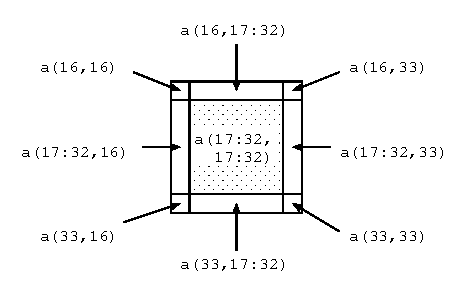
\includegraphics[width=\hsize]{figs/fig3.1.eps}
\end{center}
\caption{Example of Shadow of a Two-dimensional Array}
\label{fig3.1}
\end{figure}
\end{minipage}

\vspace{0.5cm}

The node {\tt p(2,2)} has {\tt a(17:32,17:32)} as a data object, and
{\tt a(16,16)}, {\tt a(17:32,16)}, {\tt a(33,16)}, {\tt a(16,17:32)},
{\tt a(33,17:32)}, {\tt a(16,33)}, {\tt a(17:32,33)} and {\tt a(33,33)}
as shadow objects (Figure \ref{fig3.1}). Among them, {\tt a(16,16)},
{\tt a(33,16)}, {\tt a(16,33)} and {\tt a(33,33)} are
``obliquely-neighboring'' elements of {\tt p(2,2)}.


\subsection{{\tt template\_fix} Construct}
\label{subsec:template_fix directive}

\subsubsection*{Synopsis}

This construct fixes the shape and/or the distribution of an undefined
template.

\subsubsection*{Syntax}
\Syntax{template\_fix}

\begin{tabular}{ll}
\verb![F]! & \verb|!$xmp| {\tt template\_fix} {\openb}\verb|(| {\it
 dist-format} {\openb}, {\it dist-format}{\closeb}... \verb|)|{\closeb}
 {\bsquare} \\
 & \hspace{3cm}{\bsquare} {\it template-name} {\openb}\verb|(|{\it
     template-spec} {\openb}, {\it
     template-spec}{\closeb}... \verb|)|{\closeb} \\
& \\
\verb![C]! & \verb|#pragma xmp|  {\tt template\_fix} {\openb}\verb|(|
     {\it dist-format} {\openb}, {\it
     dist-format}{\closeb}...\verb|)|{\closeb} {\bsquare} \\
 & \hspace{3cm}{\bsquare} {\it template-name} {\openb}\verb|(|{\it template-spec} {\openb}, {\it template-spec}{\closeb}... \verb|)|{\closeb} \\
 & \hspace{4cm} or \\
 & \hspace{3cm}{\bsquare} {\it template-name} \verb|[| {\it template-spec} \verb|]|
     {\openb} \verb|[|{\it template-spec} \verb|]|... {\closeb} \\
\end{tabular}
\vspace{0.3cm}

where {\it template-spec} is:

\vspace{0.3cm}

\begin{tabular}{ll}
 \hspace{0.5cm} & {\openb}{\it int-expr} :{\closeb} {\it int-expr} \\
\end{tabular}
\vspace{0.3cm}

and {\it dist-format} is one of:

\vspace{0.3cm}

\begin{tabular}{ll}
 \hspace{0.5cm} & {\tt *} \\
 & {\tt block} {\openb}\verb|(| {\it int-expr} \verb|)|{\closeb} \\
 & {\tt cyclic} {\openb}\verb|(| {\it int-expr} \verb|)|{\closeb} \\
 & {\tt gblock} \verb|(| {\it int-array} \verb|)| \\
\end{tabular}

\subsubsection*{Description}

The {\tt template\_fix} construct fixes the shape and/or the
distribution of the template that is initially undefined, by specifying
the sizes and/or the distribution format of 
each dimension at runtime. Arrays aligned with an initially undefined
template must be an allocatable array, in {\XMPF}, or a pointer (see
Section \ref{sec:Dynamic Allocation of Global Data in C}), in
{\XMPC}, which cannot be allocated until the template is fixed by the
{\tt template\_fix} construct. Any constructs that have such a
template in their {\tt on} clause must not be encountered until the
template is fixed by the {\tt template\_fix} construct. Any undefined
template can be fixed only once by the {\tt template\_fix} construct in
its scoping unit.

The meaning of the sequence of {\it dist-format}'s is the same
as that in the {\tt distribute} directive.

\subsubsection*{Restrictions}

\begin{itemize}
% \item \verb![C]! {\it template-name} must be declared by a {\tt
%       template} directive that lexically precedes the directive.
% \item \verb![C]! {\it nodes-name} must be declared by a {\tt nodes}
%       directive that lexically precedes the directive.
\item When a node encounters a {\tt template\_fix} construct at runtime,
      the template specified by {\it template-name} must be undefined.
\item If the sequence of {\it dist-format}'s exists in a {\tt
      template\_fix} construct, it must be identical with the 
      sequence of {\it dist-format}'s in the {\tt distribute} directive
      for the template specified by {\it template-name}, except for {\it
      int-array} specified in the parenthesis following {\tt gblock}.
\item Either the sequence of {\it dist-format}'s or the sequence of {\it
      template-spec}'s must be given. 
%\item The {\tt template\_fix} construct must appear in executable
%      context.
\end{itemize}

\subsubsection*{Example}
\Example{template\_fix}

\vspace{0.5cm}
\begin{minipage}{0.45\hsize}
\begin{center}
\begin{XFexample}
!$xmp template t(:)
!$xmp distribute t(gblock(*))
real, allocatable :: a(:)
!$xmp align a(i) with t(i)
...
N = ...
M(...) = ...
...
!$xmp template_fix(gblock(M)) t(N)
...
allocate (a(N))
\end{XFexample}
\end{center}
\end{minipage}
%
\begin{minipage}{0.52\hsize}
\begin{center}
\begin{XCexampleR}
#pragma xmp template t[:]
#pragma xmp distribute t[gblock(*)]
double *a;
#pragma xmp align a[i] with t[i]
...
N = ...;
M[] = {...};
...
#pragma xmp template_fix(gblock(M)) t[N]
...
a = xmp_malloc(xmp_desc_of(a), N);
\end{XCexampleR}
\end{center}
\end{minipage}

Since the shape is {\tt t(:)} or {\tt t[:]} and the distribution format is {\tt gblock(*)}, 
the template {\tt t} is initially undefined. The allocatable array
{\tt a} is aligned with {\tt t}. After the size {\tt N} and the
mapping array {\tt M} is defined, {\tt t} is fixed by the {\tt
  template\_fix} construct and {\tt a} is allocated.


In {\XMPC}, it is possible to allocate global arrays at runtime only
when they are one-dimensional.
%
Such allocation is done through the following steps.
%
\begin{enumerate}
 \item Declare a pointer to an object of the type of the global array to
       be allocated.
 \item Align the pointer with a template as if it were a one-dimensional
       array.
 \item Allocate a storage of the global size with the function {\tt xmp\_malloc()}
       and assign the result value to the pointer on each node.
\end{enumerate}
%
The functions {\tt xmp\_desc\_of()} and {\tt xmp\_malloc()} are described in section 
\ref{sec:Descriptor of Global Data in C} and \ref{subsec: xmp_malloc}, respectively.


\section{Work Mapping Construct}

\subsection{{\tt task} Construct}

\subsubsection*{Synopsis}

The {\tt \Directive{task}} construct defines a task that is executed by
a specified node set.

\subsubsection*{Syntax}
\Syntax{task}

\begin{tabular}{ll}
\verb![F]! & \verb|!$xmp| {\tt task on} \{{\it nodes-ref} $\vert$ {\it
 template-ref}\} \\
& {\it structured-block} \\
& \verb|!$xmp| {\tt end task} \\
& \\
\verb![C]! & \verb|#pragma xmp| {\tt task on} \{{\it nodes-ref} $\vert$
     {\it template-ref}\} \\
& {\it structured-block} \\
\end{tabular}

\subsubsection*{Description}

When a node encounters a {\tt task} construct at runtime, it executes
the associated block (called a {\it task}) if it is included by the node
set specified by the {\tt on} clause; otherwise, it skips the execution
of the block.

%This line was inserted by Sakagami for svn test. 

Unless a {\tt task} construct is surrounded by a {\tt \Directive{tasks}}
construct, {\it nodes-ref} or {\it template-ref} in the {\tt on} clause
is evaluated by the executing node set at the start of the task;
otherwise, {\it nodes-ref} and {\it template-ref} of the {\tt task}
construct are evaluated by the executing node set at the entry of the
{\tt tasks} construct that immediately surrounds it.
%where the evaluation
%results must be the same in every node in the executing node set.
%
The current executing node set is set to be that specified by the {\tt
on} clause at the entry of the {\tt task} construct, and it is rewound
to the last one at the exit.

%When {\it nodes-ref} or {\it template-ref} is evaluated, the
%corresponding new executing node set is created conceptually.

%The former
%executing node set that includes the node encountering the {\tt task}
%construct is referred to as the ``\Term{parent executing node set}'' of
%the new executing node set.

\subsubsection*{Restrictions}

\begin{itemize}
\item The node set specified by {\it nodes-ref} or {\it template-ref}
      in the {\tt on} clause must be a subset of the parent node set.
\end{itemize}

\subsubsection*{Example}
\Example{task}
\Example{end task}

\begin{description}

\item[Example 1]

In XcalableMP Fortran, copies of variables {\tt a} and {\tt b} are replicated on
nodes {\tt nd(1)} through {\tt nd(8)}. 
A task defined by the {\tt task} construct is executed only on {\tt nd(1)}, and
defines the copies of {\tt a} and {\tt b} on a node {\tt nd(1)}. 
The copies on nodes {\tt nd(2)} through {\tt nd(8)} are not defined.

In XcalableMP C, copies of variables {\tt a} and {\tt b} are replicated on
nodes {\tt nd[0]} through {\tt nd[7]}. 
A task defined by the {\tt task} construct is executed only on {\tt nd[0]}, and
defines the copies of {\tt a} and {\tt b} on a node {\tt nd[0]}.
The copies on nodes {\tt nd[1]} through {\tt nd[7]} are not defined.

\hspace{\hsize}

\begin{minipage}{0.44\hsize}
\begin{center}
\begin{XFexample}
!$xmp nodes nd(8)
!$xmp template t(100)
!$xmp distribute t(block) onto nd

      real a, b;

!$xmp task on nd(1)
      read(*,*) a
      b = a*1.e-6
!$xmp end task
\end{XFexample}
\end{center}
\end{minipage}
%
\begin{minipage}{0.51\hsize}
\begin{center}
\begin{XCexampleR}
#pragma xmp nodes nd[8]
#pragma xmp template t[100]
#pragma xmp distribute t[block] onto nd

    float a, b;

#pragma xmp task on nd[0]
    {
        scanf ("%f", &a);
        b = a*1.e-6;
    }
\end{XCexampleR}
\end{center}
\end{minipage}

\vspace{1cm}

\item[Example 2]

According to the {\tt on} clause with a template reference,
an assignment statement in the {\tt task} construct is
executed by the owner of the array element {\tt a(:,j)} or {\tt a[j][:]}.

\hspace{\hsize}

\begin{minipage}{0.44\hsize}
\begin{center}
\begin{XFexample}
!$xmp nodes nd(8)
!$xmp template t(100)
!$xmp distribute t(block) onto nd

      integer i,j
      real a(200,100)
!$xmp align a(*,j) with t(j)

      i = ...
      j = ...

!$xmp task on t(j)
      a(i,j) = 1.0
!$xmp end task
\end{XFexample}
\end{center}
\end{minipage}
%
\begin{minipage}{0.51\hsize}
\begin{center}
\begin{XCexampleR}
#pragma xmp nodes nd[8]
#pragma xmp template t[100]
#pragma xmp distribute t(block) onto nd

    int i,j;
    float a[100][200];
#pragma align a[j][*] with t[j]

    i = ...;
    j = ...;

#pragma xmp task on t[j]
    a[j][i] = 1.0;
}
\end{XCexampleR}
\end{center}
\end{minipage}

\end{description}


\subsection{{\tt tasks} Construct}

\subsubsection*{Synopsis}

The {\tt \Directive{tasks}} construct is used to instruct the executing
nodes to execute the multiple tasks that it surrounds in an arbitrary
order.

\subsubsection*{Syntax}
\Syntax{tasks}

\begin{tabular}{ll}
\verb![F]! & \verb|!$xmp| {\tt tasks} \\
& {\it task-construct} \\
& ... \\
& \verb|!$xmp| {\tt end tasks} \\
& \\
\verb![C]! & \verb|#pragma xmp| {\tt tasks} \\
& {\tt \{} \\
& \hspace{0.5cm} {\it task-construct} \\
& \hspace{0.5cm} ... \\
& {\tt \}} \\
\end{tabular}

\subsubsection*{Description}

{\tt \Directive{task}} constructs surrounded by a {\tt tasks} construct
are executed in arbitrary order without implicit synchronization at the
start of each task.
%
As a result, if there are no overlaps between the executing node sets of
the adjacent tasks, they can be executed in parallel.

{\it nodes-ref} or {\it template-ref} of each task immediately
surrounded by a {\tt tasks} construct is evaluated by the executing node
set at the entry of the {\tt tasks} construct.

No implicit synchronization is performed at the start and end of the
{\tt tasks} construct.
%
%implicit synchronization is performed at the exit of the {\tt tasks}
%construct, which guarantees that all communications issued inside child
%tasks are completed, unless a {\tt nowait} clause is specified.

%When a {\tt nowait} clause is specified, implicit
%synchronization is not performed at the end of the {\tt tasks}
%construct. Without a {\tt nowait} clause, implicit synchronization is
%performed in order to guarantee that all communications issued inside
%child tasks are completed.

\subsubsection*{Example}
\Example{tasks}
\Example{task}
\Example{end tasks}
\Example{end task}

\begin{description}
 \item[Example 1]

	    Three instances of subroutine {\tt task1} are concurrently
	    executed by node sets {\tt p(1:500)}, {\tt p(501:800)}, and
	    {\tt p(801:1000)}.

\hspace{\hsize}

\begin{minipage}{0.45\hsize}
\begin{center}
\begin{XFexample}
      subroutine caller
!$xmp nodes p(1000)
!$xmp template tp(100)
!$xmp distribute t(block) onto p
      real a(100,100)
!$xmp align a(*,k) with t(k)
      ...
!$xmp tasks
!$xmp  task on p(1:500)
        call task1(a)
!$xmp  end task
!$xmp  task on p(501:800)
        call task1(a)
!$xmp  end task
!$xmp  task on p(801:1000)
        call task1(a)
!$xmp  end task
!$xmp end tasks
      ...
      end subroutine
\end{XFexample}
\end{center}
\end{minipage}
%
\begin{minipage}{0.45\hsize}
\begin{center}
\begin{XFexampleR}
      subroutine task1(a)
      ...
!$xmp nodes q(*)=*

!$xmp nodes p(1000)
!$xmp distribute t(block) onto p
      real a(100,100)
!$xmp align a(*,k) with t(k)
      ...
      end subroutine
\end{XFexampleR}
\end{center}
\end{minipage}

\vspace{1cm}

 \item[Example 2]

	    The first node {\tt p(1)} executes the first and second
	    tasks, the final {\tt node p(8)} the second and the third
	    tasks, and the other nodes {\tt p(2)} through {\tt p(7)}
	    only the second task.

\hspace{\hsize}

\begin{XFexample}
!$xmp nodes p(8)
!$xmp template t(100)
!$xmp distribute t(block) onto p
      real a(100)
!$xmp align a(i) with t(i)
      ...
!$xmp tasks

!$xmp task on t(1)
      a(1) = 0.0
!$xmp end task

!$xmp task on t(2:99)
!$xmp loop on t(i)
      do i=2,99
        a(i) = foo(i)
      enddo
!$xmp end task

!$xmp task on t(100)
      a(100) = 0.0
!$xmp end task

!$xmp end tasks
\end{XFexample}

\end{description}


\subsection{{\tt loop} Construct}
\label{sub:loop_construct}

\subsubsection*{Synopsis}

The {\tt \Directive{loop}} construct specifies that each iteration of
the following loop is executed by a node set that is specified by the {\tt on}
clause, so the iterations are distributed among nodes and executed
in parallel.
% where the specified data is accessed locally.
% inserted by Sakagami,H. 09/11/13
%If the loop body includes reduction operations, then they must be
%specified in the {\tt loop} directive to obtain the correct results.

\subsubsection*{Syntax}
\Syntax{loop}

\begin{tabular}{ll}
\verb![F]! & \verb|!$xmp| {\tt loop} {\openb} \verb|(| {\it loop-index}
 {\openb}, {\it loop-index}{\closeb}... \verb|)| {\closeb} 
	  {\tt on} \{{\it nodes-ref} $\vert$ {\it template-ref}\} {\bsquare} \\
 & \hspace{5cm}{\bsquare} 
	  {\openb} \verb|expand(| {\it expand-width} {\openb}, {\it
	  expand-width}{\closeb}... \verb|)| {\closeb} {\bsquare} \\
 & \hspace{5cm}{\bsquare} 
	  {\openb} \verb|margin(| {\it margin-width} {\openb}, {\it
	  margin-width}{\closeb}... \verb|)| {\closeb} {\bsquare} \\
 & \hspace{5cm}{\bsquare} 
	  {\openb} {\it reduction-clause} {\closeb}... \\
 % & \hspace{5cm}{\bsquare} 
 % 	  {\openb} \verb|pipeline(| {\it pipeline-spec} {\openb}, {\it
 % 	  pipeline-spec}{\closeb}... \verb|)| {\closeb} {\bsquare} \\
 & {\it do-loops} \\
 & \\
\verb![C]! & \verb|#pragma xmp| {\tt loop} {\openb} \verb|(| {\it
     loop-index} {\openb}, {\it loop-index}{\closeb}... \verb|)|
     {\closeb} {\tt on} \{{\it nodes-ref} $\vert$ {\it template-ref}\} {\bsquare} \\
 & \hspace{5cm}{\bsquare} 
	  {\openb} \verb|expand(| {\it expand-width} {\openb}, {\it
	  expand-width}{\closeb}... \verb|)| {\closeb} {\bsquare} \\
 & \hspace{5cm}{\bsquare} 
	  {\openb} \verb|margin(| {\it margin-width} {\openb}, {\it
	  margin-width}{\closeb}... \verb|)| {\closeb} {\bsquare} \\
 & \hspace{5cm}{\bsquare}
	  {\openb} {\it reduction-clause} {\closeb}... \\
 % & \hspace{5cm}{\bsquare} 
 % 	  {\openb} \verb|pipeline(| {\it pipeline-spec} {\openb}, {\it
 % 	  pipeline-spec}{\closeb}... \verb|)| {\closeb} {\bsquare} \\
 & {\it for-loops} \\
\end{tabular}

%\vspace{0.3cm}
%
%where {\it on-ref} is one of:
%
%\vspace{0.3cm}
%
%\begin{tabular}{ll}
% \hspace{0.5cm} & {\it template-ref} \\
% & {\it nodes-ref} \\
%\end{tabular}
%
\vspace{0.3cm}

where {\it expand-width} and {\it margin-width} must be one of:

\vspace{0.3cm}

\begin{tabular}{ll}
 \hspace{0.5cm} & {\openb}{\tt /unbound/}{\closeb} {\it int-expr} \\
                & {\openb}{\tt /unbound/}{\closeb} {\it int-expr} : {\it int-expr}
\end{tabular}

\vspace{0.3cm}


{\it reduction-clause} is:

\vspace{0.3cm}

\begin{tabular}{ll}
 \hspace{0.5cm} & \verb|reduction(| {\it reduction-kind} : {\it reduction-spec}
 {\openb}, {\it reduction-spec} {\closeb}... \verb|)| \\
\end{tabular}

\vspace{0.3cm}

{\it reduction-kind} is one of:

%�Ⴆ�΁C.AND.�́C�_���^�̕ϐ��ɑ΂��āCla = la .AND. lgcl(i)���CIAND�́C
%�����^�ϐ��ɑ΂���ia = IAND( ia, ib(i) ) ��IAND�֐����g���Ƃ��ł��D
%HPF�ɓ����Ă��܂��D���X�C���͏����Ȃ������̂ł����C�≺���񂪍폜����K
%�v���Ȃ����낤�Ƃ̂��Ƃœ���܂����D
% Reduction�w�����ɂ͓����Ă��܂��̂ŁC�lj����܂����D

\vspace{0.3cm}

\begin{tabular}{ll}
 \verb![F]! & {\tt +} \\
 & {\tt *} \\
 & {\tt -} \\
 & {\tt .and.} \\
 & {\tt .or.} \\
 & {\tt .eqv.} \\
 & {\tt .neqv.} \\
 & {\tt max} \\
 & {\tt min} \\
 & {\tt iand} \\
 & {\tt ior} \\
 & {\tt ieor} \\
 & {\tt firstmax} \\
 & {\tt firstmin} \\
 & {\tt lastmax} \\
 & {\tt lastmin} \\
 & \\
 \verb![C]! & {\tt +} \\
 & {\tt *} \\
 & {\tt -} \\
 & {\tt \verb|&|} \\
 & {\tt |} \\
 & {\tt \verb|^|} \\
 & {\tt \verb|&&|} \\
 & {\tt ||} \\
 & {\tt max} \\
 & {\tt min} \\
 & {\tt firstmax} \\
 & {\tt firstmin} \\
 & {\tt lastmax} \\
 & {\tt lastmin} \\
\end{tabular}

\vspace{0.3cm}

and {\it reduction-spec} is:

\vspace{0.3cm}

\begin{tabular}{ll}
 \hspace{0.5cm} & {\it reduction-variable} {\openb} {\tt /} {\it
 location-variable} {\openb}, {\it location-variable}
 {\closeb}... {\tt /} {\closeb} \\
\end{tabular}

% \vspace{0.3cm}

% and {\it pipeline-spec} is:

% \vspace{0.3cm}

% \begin{tabular}{ll}
%  \hspace{0.5cm} & {\it array-name} {\tt /} {\it int-expr} {\openb}, {\it
% 	  int-expr} {\closeb}... {\tt /} \\
% \end{tabular}

\subsubsection*{Description}

A {\tt loop} directive is associated with a loop nest
consisting of one or more tightly nested loops that follow the directive,
and it distributes the execution of their iterations onto the node set
specified by the {\tt on} clause.
% inserted by Sakagami,H. 09/11/13
%Since the iteration range of the loop for each node is determined before
%the loop is executed, efficient loop execution can be expected.

The sequence of {\it loop-indexes} in parenthesis denotes an index of
an iteration of the loop nests. If a control variable of a loop does
not appear in the sequence, it is assumed that each of its possible
values is specified in the sequence. The sequence can be considered to 
denote a set of indices of iterations.
%
When the sequence is omitted, it is assumed that the control variables
of all the loops in the associated loop nests are specified.

When a {\it template-ref} is specified in the {\tt on} clause, the
associated loop is distributed so that the iteration (set) indexed by
the sequence of {\it loop-indexes}  is executed by the node onto
which a template element specified by the {\it template-ref} is
distributed.

%Therefore, before the {\tt
%\Directive{loop}} construct is executed, the referenced template must be
%fixed.
%When {\it template-spec} is ``*'', the corresponding dimension is
%collapsed so that it is ignored for the distribution of the loop. When
%{\it template-spec} is ``:'', the nodes for all of the template elements
%in the corresponding dimension are assigned to iterations for execution. 

% modified by Sakagami,H. 09/11/13
When a {\it nodes-ref} is specified in the {\tt on} clause, the
associated loop is distributed so that the iteration (set) indexed by
the sequence of {\it loop-indexes} is executed by a node
specified by the {\it nodes-ref}.

In addition, the executing node set is updated to the node set specified
by the {\tt on} clause at the beginning of every iteration, and it is
restored to the last one at the end of it.

% inserted and modified by Sakagami,H. 09/11/13
%When the loop includes reduction operations, proper {\it reduction-clause}
%must be specified in order to obtain semantically correct results,
%and
%the reduction operation is executed on the specified local reduction
%variable just after the execution of the loop.

When a {\it reduction-clause} is specified, a reduction operation of the
kind specified by {\it reduction-kind} for a variable specified by
{\it reduction-variable} is executed just after the execution of the loop
nest.

% inserted by Sakagami,H. 09/11/13
%The {\tt loop} construct that has {\it template-ref} as {\it
%on-ref} and the {\tt reduction} clause, except in cases with {\it
%reduction-kind} of {\tt FIRSTMAX}, {\tt FIRSTMIN}, {\tt LASTMAX}, or
%{\tt LASTMIN}, is equivalent to the {\tt \Directive{reduction}}
%construct with the following {\it template-spec} replacements:

\mytextcolor{red}{
When the {\tt expand} clause is specified, and is of the form ``{\it
int-expr} : {\it int-expr}'' in a dimension, 
the first {\it int-expr} is subtracted from the local lower bound in
that dimension, and the second one is added to the local upper bound.
%
When the {\tt expand} clause is specified, and is of the form {\it int-expr},
the {\it int-expr} is subtracted from the local lower bound in that
dimension, and is added to the local upper bounds.
%
However, an ``expanded'' local iteration space does not spread out of
the original global iteration space unless the \Term{{\tt /unbound/}
modifier} is specified in {\it expand-width}.
}

\mytextcolor{red}{
When the {\tt margin} clause is specified, the loop is transformed so
that its local iteration space, $margin$, is:
$$margin = expand \bigtriangleup orig$$
where $expand$ is a local iteration space when an {\tt expand} clause
with the same argument(s) is specified, 
$orig$ is a local iteration space when neither $expand$ nor $margin$,
and 
$\bigtriangleup$ is the symmetric difference operator.
}

\mytextcolor{red}{
\begin{quotation}
  (Advice to programmers and implementers) Using the {\tt expand} and
  {\tt margin} clauses and asynchronous communication, programmers can
  overlap computation and communication as in the code left
  below. It is recommended for the implementation to support an
  extension that is a syntactic sugar for those sequence of constructs,
  such as the {\tt peel\_and\_wait} clause in the code immediately
  following.
\end{quotation}
}

\vspace{1zw}

\begin{minipage}{0.45\hsize}
\begin{center}
\begin{XFexample}
!$xmp reflect (a) async(10)

!$xmp loop (i,j) on t(i,j)
!$xmp+              expand(-1,-1)
      do j = 1, 16
          do i = 1, 16
              ...
          end do
      end do

!$xmp wait_async (10)

!$xmp loop (i,j) on t(i,j)
!$xmp+              margin(-1,-1)
      do j = 1, 16
          do i = 1, 16
              ...
          end do
      end do
\end{XFexample}
\end{center}
\end{minipage}
%
\begin{minipage}{0.45\hsize}
\begin{center}
\begin{XFexampleR}
!$xmp reflect (a) async(10)

!$xmp loop (i,j) on t(i,j)
!$xmp+   peel_and_wait(10, -1,-1)
      do j = 1, 16
          do i = 1, 16
              ...
          end do
      end do
\end{XFexampleR}
\end{center}
\end{minipage}

\vspace{1zw}

The reduction operation that is executed, except in cases with {\it
reduction-kind} of {\tt FIRSTMAX}, {\tt FIRSTMIN}, {\tt LASTMAX}, or
{\tt LASTMIN},
\mytextcolor{red}{
is equivalent to the {\tt reduction}
construct with {\it reduction-kind} of ``{\tt +}'' for ``{\tt -}'' in
the clause and the same {\it reduction-kind} for the other kinds},
 the same {\it
reduction-variable}, and an {\tt on} clause obtained from that of the
{\tt loop} directive by replacing each {\it loop-index} in the {\it
nodes-ref} or the {\it template-ref} with a triplet representing the
range of its value.
% replacing:
% %
% \begin{itemize}
%  \item ``{\tt :}'' in the {\it nodes-ref} or the {\it template-ref} with
%        ``{\tt *}'', and
%  \item {\it loop-index} in the {\it nodes-ref} or the {\it template-ref}
%        with a triplet representing the range of its value.
% \end{itemize}
%
As an example, the two codes below are therefore equivalent.

\vspace{1zw}

\Example{loop}
\begin{minipage}{0.45\hsize}
\begin{center}
\begin{XFexample}
!$xmp loop (j) on t(:,j)
!$xmp+             reduction(op:s)
      do j = js, je
        ...
        do i = 1, N
          s = s op a(i,j)
        end do
        ...
      end do
\end{XFexample}
\end{center}
\end{minipage}
%
\begin{minipage}{0.46\hsize}
\begin{center}
\begin{XFexampleR}
! Initialize s_tmp to the identity
! element of the op operator
      s_tmp = ...

!$xmp loop (j) on t(:,j) 
      do j = js, je
        ...
        do i = 1, N
          s_tmp = s_tmp op a(i,j)
        end do
        ...
      end do

!$xmp reduction(op:s_tmp)
!$xmp+               on t(*,js:je)

      s = s op s_tmp
\end{XFexampleR}
\end{center}
\end{minipage}

\vspace{1zw}

In particular, for the reduction kinds of {\tt FIRSTMAX}, {\tt FIRSTMIN},
{\tt LASTMAX}, and {\tt LASTMIN}, in addition to a corresponding {\tt
MAX} or {\tt MIN} reduction operation, the {\it
location-variables}\index{location-variable} are set after executing the
{\tt loop} construct as follows:
%
\begin{itemize}
 \item For {\tt FIRSTMAX} and {\tt FIRSTMIN}, they are set to their
       values at the end of the {\it first} iteration in which
       the {\it reduction-variable} takes the value of the reduction
       result, where {\it first} refers to the first position in the
       sequential order in 
       which iterations of the associated loop nest were executed
       without parallelization.
 \item For {\tt LASTMAX} and {\tt LASTMIN}, they are set to their
       values at the end of the {\it last} iteration in which
       the {\it reduction-variable} takes the value of the reduction
       result, where {\it last} refers to the last position in the
       sequential order in 
       which iterations of the associated loop nest were executed
       without parallelization.
\end{itemize}

% inserted by Sakagami,H. 09/11/13 ----- start ---
%Note that, unlike a {\tt \Directive{loop}} construct with the {\tt
%reduction} clause, a {\tt \Directive{reduction}} construct does not
%consider initialization for the reduction variable.  The following
%programs return different values of the {\tt sum} variable after the
%reduction operation. When {\tt sum} is initialized to zero, these
%programs return the same results.
%
%\vspace{1zw}
%
%\begin{minipage}{0.45\hsize}
%\begin{center}
%\begin{XFexample}
%      sum = 123.45
%!$xmp loop (i) on t(i)
%!$xmp+            reduction(+:sum)
%      do i = 1, N
%         sum = sum + a(i)
%      end do
%\end{XFexample}
%\end{center}
%\end{minipage}
%%
%\begin{minipage}{0.45\hsize}
%\begin{center}
%\begin{XFexampleR}
%      sum = 123.45
%!$xmp loop (i) on t(i)
%      do i = 1, N
%         sum = sum + a(i)
%       end do
%!$xmp reduction(+:sum) on t(1:N)
%\end{XFexampleR}
%\end{center}
%\end{minipage}
% inserted by Sakagami,H. 09/11/13 ----- end ---

% \mytextcolor{red}{
% When the {\tt pipeline} clause is specified, the distributed loop nest is
% executed by nodes in such a pipeline manner that 
% %
% each node waits until recieving from, executes its own local part of the loop nest, and
% then sends, to resolve loop-carried dependence.
% }

\subsubsection*{Restrictions}

\begin{itemize}
 \item {\it loop-index} must be a control variable of a loop in the
       associated loop nest.
 \item A control variable of a loop can appear as {\it loop-index} at
       most once.
% \item {\it template-spec} appearing in {\it template-ref} must be
%       either ``*'', ``:'', or {\it loop-index}.
%       In the case of {\it
%       loop-index}, the loop index must be the loop index of the outer
%       loop of the loop.
% \item {\it nodes-ref} must reference different node sets for each {\it
%       loop-index}. These node sets consist of different nodes. That is,
%       a node must not be included in more than one node set. 

 \item The node set specified by {\it nodes-ref} or {\it template-ref}
       in the {\tt on} clause must be a subset of the parent node set.

 \item The template specified by {\it template-ref} must be fixed 
       before the {\tt loop} construct is executed.

 % \item The {\tt loop} construct is global, which means that it must be
 %       executed by all of the executing nodes, and each local variable
 %       referenced in the directive must have the same value among all of
 %       them, and the lower bound, upper bound, and step of the
 %       associated loop must have the same value among all of them.

 \item The {\tt loop} construct is global, which means that it must be
       executed by all of the executing nodes with the same values for
       each local variable referenced in the directive, and the lower
       bound, upper bound, and step of the associated loop.

 \item \mycolor{red}{Either of the {\tt expand} or {\tt margin} clause,
	   if any, can be specified.}

 \item The number of {\it expand-width}, if any, must be equal to the
	   number of dimensions (or rank) of the template specified by {\it
	   template-ref} or of the node array specified by {\it node-ref}.

 \item The number of {\it margin-width}, if any, must be equal to the
	   number of dimensions (or rank) of the template specified by {\it
	   template-ref} or of the node array specified by {\it node-ref}.
	   \mycolor{black}{}

% modified by Sakagami,H. 09/11/13
 \item {\it reduction-spec} must have one or more {\it
       location-variable}'s if and only if {\it reduction-kind} is
       either {\tt FIRSTMAX}, {\tt FIRSTMIN}, {\tt LASTMAX}, or {\tt
       LASTMIN}.

 % \item \mycolor{red}{The array specified by {\it array-name} in {\it
 %       pipeline-spec} must be mapped onto the executing node set.}

 % \item \mycolor{red}{The number of {\it int-expr} in {\it pipeline-spec}
 % 	   must be equal to the number of dimensions (or rank) of the array
 % 	   specified by {\it array-name} in {\it pipeline-spec}.}

% inserted by Sakagami,H. 09/11/13
%\item {\it reduction-clause} must reference the reduction operations
%      associated with the loop after the directive or the loops nested
%      by the loop.

% \item {\it location-variable} must be fixed in the loop after the
%       directive or the loops nested by the loop.

%\item {\it reduction-variable} must not be referred at a certain
%      iteration in the loop, except for updating itself.

% \item {\it reduction-variable} and {\it location-variable} must not
%       exist in {\it reduction-clause} of nested loops.

\end{itemize}

\subsubsection*{Examples}
\Example{loop}

\begin{description}
\item[Example 1]
\hspace{\hsize}
\begin{XFexample}
!$xmp distribute t(block) onto p
!$xmp align (i) with t(i) :: a, b
      ...
!$xmp loop (i) on t(i)
      do i = 1, N
          a(i) = 1.0
          b(i) = a(i)
      end do
\end{XFexample}

The {\tt loop} construct determines the node that executes each
of the iterations, according to the distribution of template {\tt t}, and
distributes 
the execution. This example is syntactically equivalent to the one
shown below, but will be faster because the iterations to be executed by
each node can be determined before executing the loop.

\Example{task}
\begin{XFexample}
!$xmp distribute t(block) onto p
!$xmp align (i) with t(i) :: a, b
      ...
      do i = 1, N
!$xmp task on t(i)
          a(i) = 1.0
          b(i) = a(i)
!$xmp end task
      end do
\end{XFexample}

\item[Example 2]
\hspace{\hsize}
\begin{XFexample}
!$xmp distribute t(*,block) onto p
!$xmp align (i,j) with t(i,j) :: a, b
      ...
!$xmp loop (i,j) on t(i,j)
      do j = 1, M
          do i = 1, N
              a(i,j) = 1.0
              b(i,j) = a(i,j)
          end do
      end do
\end{XFexample}

	   Because the first dimension of template {\tt t} is not
	   distributed, only the {\tt j} loop, which is aligned with the
	   second dimension of {\tt t}, is distributed. This example is
	   syntactically equivalent to the {\tt task} construct shown
	   below.

\Example{task}
\begin{XFexample}
!$xmp distribute t(*,block) onto p
!$xmp align (*,j) with t(*,j) :: a, b
      ...
      do j = 1, M
!$xmp task on t(*,j)
          do i = 1, N
              a(i,j) = 1.0
              b(i,j) = a(i,j)
          end do
!$xmp end task 
      end do
\end{XFexample}

\item[Example 3]
\hspace{\hsize}
\begin{XFexample}
!$xmp distribute t(block,block) onto p
!$xmp align (i,j) with t(i,j) :: a, b
      ...
!$xmp loop (i,j) on t(i,j)
      do j = 1, M
          do i = 1, N
              a(i,j) = 1.0
              b(i,j) = a(i,j)
          end do
      end do
\end{XFexample}

% modified by Sakagami,H. 09/11/13
The distribution of loops in the nested loop can be specified
using the sequence of {\it loop-indexes} in one {\tt loop}
construct. This example is equivalent to the loop shown
below, but will run faster because the iterations 
to be executed by each node can be determined outside of the nested
loop. Note that the node set specified by the inner {\tt on}
clause is a subset of that specified by the outer one.

\begin{XFexample}
!$xmp distribute t(block,block) onto p
!$xmp align (i,j) with t(i,j) :: a, b
      ...
!$xmp loop (j) on t(:,j)
      do j = 1, M
!$xmp loop (i) on t(i,j)
          do i = 1, N
              a(i,j) = 1.0
              b(i,j) = a(i,j)
          end do
      end do
\end{XFexample}

\item[Example 4]
\hspace{\hsize}

\begin{XFexample}
!$xmp nodes p(10,3)
      ...
!$xmp loop on p(:,i)
      do i = 1, 3
          call subtask ( i )
      end do
\end{XFexample}

	   Three node sets {\tt p(:,1)}, {\tt p(:,2)}, and {\tt p(:,3)}
	   are created as the executing node sets, and each of them
	   executes iterations {\tt 1}, {\tt 2}, and {\tt 3} of the
	   associated loop, respectively.
%
This example is equivalent to the loop
% modified by Sakagami,H. 09/11/13
containing {\tt task} constructs (below left) or static {\tt tasks/task}
constructs (below right).

\vspace{0.5cm}

\begin{minipage}{0.45\hsize}
\begin{center}
\begin{XFexample}
!$xmp nodes p(10,3)
      ...
      do i = 1, 3
!$xmp task on p(:,i)
          call subtask ( i )
!$xmp end task
      end do
\end{XFexample}
\end{center}
\end{minipage}
\begin{minipage}{0.45\hsize}
\begin{center}
\begin{XFexampleR}
!$xmp nodes p(10,3)
      ...
!$xmp tasks
!$xmp task on p(:,1)
      call subtask ( 1 )
!$xmp end task
!$xmp task on p(:,2)
      call subtask ( 2 )
!$xmp end task
!$xmp task on p(:,3)
      call subtask ( 3 )
!$xmp end task
!$xmp end tasks
\end{XFexampleR}
\end{center}
\end{minipage}
\vspace{1cm}

\item[Example 5]
\hspace{\hsize}
\begin{XFexample}
      ...
      lb(1)  = 1
      iub(1) = 10
      lb(2)  = 11
      iub(2) = 25
      lb(3)  = 26
      iub(3) = 50
!$xmp loop (i) on p(lb(i):iub(i))
      do i = 1, 3
          call subtask ( i )
      end do
\end{XFexample}

The executing node sets of different sizes are created by
{\tt p(lb(i):iub(i))} with different values of i for unbalanced workloads. This example is equivalent to the loop containing 
% modified by Sakagami,H. 09/11/13
{\tt task} constructs (below left) or static {\tt
	   tasks/task} constructs (below right).

\vspace{1cm}

\begin{minipage}{0.45\hsize}
\begin{center}
\begin{XFexample}
      do i = 1, 3
!$xmp task on p(lb(i):iub(i))
          call subtask ( i )
!$xmp end task
      end do
      ...
\end{XFexample}
\end{center}
\end{minipage}
\begin{minipage}{0.45\hsize}
\begin{center}
\begin{XFexampleR}
!$xmp tasks
!$xmp task on p(1:10)
      call subtask ( 1 )
!$xmp end task
!$xmp task on p(11:25)
      call subtask ( 2 )
!$xmp end task
!$xmp task on p(25:50)
      call subtask ( 3 )
!$xmp end task
!$xmp end tasks
\end{XFexampleR}
\end{center}
\end{minipage}
\vspace{1cm}

\item[Example 6]
\hspace{\hsize}
\begin{XFexample}
      ...
      s = 0.0
!$xmp loop (i) on t(i) reduction(+:s)
      do i = 1, N
          s = s + a(i)
      end do
\end{XFexample}

This loop computes the sum of {\tt a(i)} into the variable {\tt s} on
each node. Note that only the partial sum is computed on {\tt s} without
the reduction clause. This example is equivalent to the code given below. 

\begin{XFexample}
      ...
      s = 0.0
!$xmp loop (i) on t(i) 
      do i = 1, N
          s = s + a(i)
      end do
!$xmp reduction(+:s) on t(1:N)
\end{XFexample}

\item[Example 7]
\hspace{\hsize}
\begin{XFexample}
      ...
      amax = -1.0e30
      ip = -1
      jp = -1
!$xmp loop (i,j) on t(i,j) reduction(firstmax:amax/ip,jp/)
      do j = 1, M
          do i = 1, N
              if( 1(i,j) .gt. amx ) then
                  amx = a(i,j)
                  ip = i
                  jp = j
              end if
          end do
      end do
\end{XFexample}

	   This loop computes the maximum value of {\tt a(i,j)} and
	   stores it into the variable {\tt amax} in each node. In
	   addition, the first indices for the maximum element of {\tt
	   a} are obtained in {\tt ip} and {\tt jp} after executing the
	   loops.
% inserted by Sakagami,H. 09/11/13
	   Note that this example cannot be written using the {\tt
	   reduction} construct.
% modified by Sakagami,H. 09/11/13

\item[Example 8]
\hspace{\hsize}
\mycolor{red}{
\begin{XFexample}
!$xmp loop (i,j) on t(i,j) expand(/unbound/1,/unbound/1)
      do j = 1, 16
          do i = 1, 16
              ...
          end do
      end do

!$xmp loop (i,j) on t(i,j) margin(/unbound/1,/unbound/1)
      do j = 1, 16
          do i = 1, 16
              ...
          end do
      end do
\end{XFexample}

		   Assuming that the template {\tt t(100,100)} is distributed in
		   (block,block) onto a node array {\tt p(4,4)}, the original local
		   iteration space on {\tt p(1,1)}, $orig_{1,1}$ is:
		   \[
		   \begin{array}{lllll}
			 orig_{1,1} = \{ & (1,1), & (2,1), & (3,1), & (4,1), \\
			                 & (1,2), & (2,2), & (3,2), & (4,2), \\
			                 & (1,3), & (2,3), & (3,3), & (4,3), \\
		                     & (1,4), & (2,4), & (3,4), & (4,4) \quad \}
		   \end{array}			 
		   \]
		   and it is expanded using the {\tt expand} clause for the first
		   loop, as follows:
		   \[
		   \begin{array}{lllllll}
			 expand(1,1)_{1,1} = \{ & (0,0), & (0,1), & (0,2), & (0,3), & (0,4), & (0,5), \\
			                        & (1,0), & (1,1), & (1,2), & (1,3), & (1,4), & (1,5), \\
			                        & (2,0), & (2,1), & (2,2), & (2,3), & (2,4), & (2,5), \\
			                        & (3,0), & (3,1), & (3,2), & (3,3), & (3,4), & (3,5), \\
			                        & (4,0), & (4,1), & (4,2), & (4,3), & (4,4), & (4,5), \\
			                        & (5,0), & (5,1), & (5,2), & (5,3), & (5,4), & (5,5) \quad \}
		   \end{array}			 
		   \]
		   Note that $expand(1,1)_{1,1}$ spreads out of the original
		   global iteration space $\{ (i,j) \, | \, 1 \le i,j \le 16 \}$
		   because the {\tt /unbound/} specifier is specified in the
		   {\tt expand} clause.

		   The local iteration space for the second loop with the {\tt
		   margin} clause is defined using the symmetric difference
		   operator, as follows:
		   \[
		   \begin{array}{lllllllll}
			 margin(1,1)_{1,1} &=& \multicolumn{7}{l}{expand(1,1)_{1,1} \triangle orig_{1,1}} \\
		                       &=& \{ & (0,0), & (0,1), & (0,2), & (0,3), & (0,4), & (0,5), \\
			                   & &    & (1,0), &        &        &        &        & (1,5), \\
			                   & &    & (2,0), &        &        &        &        & (2,5), \\
			                   & &    & (3,0), &        &        &        &        & (3,5), \\
			                   & &    & (4,0), &        &        &        &        & (4,5), \\
			                   & &    & (5,0), & (5,1), & (5,2), & (5,3), & (5,4), & (5,5) \quad \}
		   \end{array}			 
		   \]
}
\end{description}


\subsection{{\tt array} Construct}

\subsubsection*{Synopsis}

The {\tt \Directive{array}} construct divides the work of an array
assignment between nodes.

\subsubsection*{Syntax}
\Syntax{array}

\begin{tabular}{ll}
\verb![F]! & \verb|!$xmp| {\tt array on} {\it template-ref} \\
 & {\it array-assignment-statement} \\
 & \\
\verb![C]! & \verb|#pragma xmp| {\tt array on} {\it template-ref} \\
 & {\it array-assignment-statement} \\
\end{tabular}

\subsubsection*{Description}

The array assignment is an alternative to a loop that performs
an assignment to each element of an array.
%
This directive specifies the parallel execution of an array assignment,
where each sub-assignment and sub-operation of an element is executed by
a node that is determined by the {\tt on} clause.

%The array assignment can be used instead of the loop of the assignment
%for each element. This directive executes the array assignment in each
%node.

Note that array assignments can also be used in {\XMPC}, which is one of
the language extensions introduced by {\XMP} (see Section \ref{sec:Array
assignment statements in C}).

% inserted by Sakagami,H. 09/11/13 --- start ---
\subsubsection*{Restrictions}

\begin{itemize}
 \item The node set specified by {\it template-ref} in the {\tt on}
       clause must be a subset of the parent node set.
 \item The template section specified by {\it template-ref} must have
       the same shape as the associated array assignment.
 %\item If the range in {\it template-ref} is omitted, all of the ranges
 %      are assumed to be specified.
 % \item The {\tt \Directive{array}} construct is global and must be
 %       executed by all of the executing nodes, and the variables
 %       that appear in the construct must all have the same value among
 %       all of them.
 \item The {\tt \Directive{array}} construct is global and must be
       executed by all of the executing nodes with the same valuse for
       the variables that appear in the construct.
\end{itemize}
% inserted by Sakagami,H. 09/11/13 --- end ---

\subsubsection*{Examples}
\Example{array}

\begin{description}

\item[Example 1]
\hspace{\hsize}

\begin{XFexample}
!$xmp distribute t(block) onto p
!$xmp align (i) with t(i) :: a
      ...
!$xmp array on t(1:N)
      a(1:N) = 1.0
\end{XFexample}

This example is equivalent to the code shown below.

\begin{XFexample}
!$xmp distribute t(block) onto p
!$xmp align (i) with t(i) :: a
      ...
!$xmp loop on t(1:N)
      do i = 1, N
          a(i) = 1.0
      end do
\end{XFexample}

% inserted by Sakagami,H. 09/11/13 --- start ---
\item[Example 2]
\hspace{\hsize}
\begin{XFexample}
!$xmp template t(100,20)
!$xmp distribute t(block,block) onto p
      dimension a(100,20), b(100,20)
!$xmp align (i,j) with t(i,j) :: a, b
      ...
!$xmp array on t
      a = b + 2.0
\end{XFexample}

This example is equivalent to the code shown below.

\begin{XFexample}
!$xmp template t(100,20)
!$xmp distribute t(block,block) onto p
      dimension a(100,20), b(100,20)
!$xmp align (i,j) with t(i,j) :: a, b
      ...
!$xmp loop (i,j) on t(i,j)
      do j = 1, 20
         do i = 1, 100
            a(i,j) = b(i,j) + 2.0
         end do
      end do
\end{XFexample}
\end{description}
% inserted by Sakagami,H. 09/11/13 --- end ---

\section{Global-view Communication and Synchronization Constructs}

\subsection{{\tt reflect} Construct} \label{sub:reflect}

\subsubsection*{Synopsis}
The {\tt \Directive{reflect}} construct assigns the value of a
reflection source to the corresponding shadow object.

\subsubsection*{Syntax}
\Syntax{reflect}
\begin{tabular}{ll}
 \verb![F]! & \verb|!$xmp| {\tt reflect} \verb|(| {\it array-name}
 {\openb}, {\it array-name}{\closeb}... \verb|)| {\bsquare} \\
 &\hspace{0.3cm} {\bsquare} {\openb}{\tt width (} {\it reflect-width}
     {\openb}, {\it reflect-width}{\closeb}... {\tt )}{\closeb}
     {\openb}{\tt orthogonal}{\closeb}
     {\openb}{\tt async (} {\it async-id} {\tt )}{\closeb} \\
\verb![C]! & \verb|#pragma xmp| {\tt reflect} \verb|(| {\it array-name}
     {\openb}, {\it array-name}{\closeb}... \verb|)| {\bsquare} \\
 &\hspace{0.3cm} {\bsquare} {\openb}{\tt width (} {\it reflect-width}
     {\openb}, {\it reflect-width}{\closeb}... {\tt )}{\closeb}
     {\openb}{\tt orthogonal}{\closeb}
     {\openb}{\tt async (} {\it async-id} {\tt )}{\closeb} \\
\end{tabular}

\vspace{0.3cm}

where {\it reflect-width} must be one of:

\vspace{0.3cm}

\begin{tabular}{ll}
 \hspace{0.5cm} & {\openb}{\tt /periodic/}{\closeb} {\it int-expr} \\
                & {\openb}{\tt /periodic/}{\closeb} {\it int-expr} : {\it int-expr}
\end{tabular}

\subsubsection*{Description}

The {\tt reflect} construct updates each of the shadow objects of the
array specified by {\it array-name} with the value of its corresponding
reflection source. Note that the shadow objects corresponding to
elements at the non-orthogonal positions are also updated with this
construct, unless the {\tt orthogonal} clause is specified.

%copies the value of the reflection source of
%the reflect-object specified by {\it array-name} to all shadow
%objects.
%This directive may execute the communications.

When the {\tt width} clause is specified and takes the form ``{\it
int-expr} : {\it int-expr}'' in a dimension, the shadow area having the
width specified by the first {\it int-expr} at the lower bound and that
specified by the second one at the upper bound in the dimension are
updated.
%
When the {\tt width} clause is specified, and takes the form {\it int-expr},
the shadow areas having the same width specified at both the upper
and lower bounds in the dimension are updated.
%
When the {\tt width} clause is omitted, the whole shadow area of the array
is updated.

In particular, when the \Term{{\tt /periodic/} modifier} is specified in
{\it reflect-width}, the update of the shadow object in the dimension is
``periodic,'' which means that the shadow object at the global lower
(upper) bound is treated as if it corresponds to the data object of the
global upper (lower) bound, and is updated with that value by the {\tt
reflect} construct.

When the {\tt orthogonal} clause is specified, only the shadow objects
corresponding to elements at the orthogonal positions are updated by the
{\tt reflect} construct.
%the shadow object is updated only by orthogonal nodes.

When the {\tt async} clause is specified, the statements following this
construct may be executed before the operation is complete.

\subsubsection*{Restrictions}

\begin{itemize}
 \item The arrays specified by the sequence of {\it array-names} must
       be mapped onto the executing node set.
 \item The reflect width of each dimension specified by the {\it
       reflect-width} must not exceed the shadow width of the arrays.
 \item The {\tt reflect} construct is global, which means that it must be
       executed by all nodes in the current executing node set, and each local
       variable referenced in the construct must have the same value
       among all of them.
 \item {\it async-id} must be an expression of type default integer in
       {\XMPF} or type {\tt int} in {\XMPC}.
\end{itemize}

\subsubsection*{Example}
\Example{reflect}
\Example{shadow}

\begin{XFexample}
!$xmp nodes p(4)
!$xmp template t(100)
!$xmp distribute t(block) onto p

      real a(100)
!$xmp align a(i) with t(i)
!$xmp shadow a(1)

      ...
!$xmp reflect (a) width (/periodic/1)
\end{XFexample}

\begin{myfigure}
\begin{center}
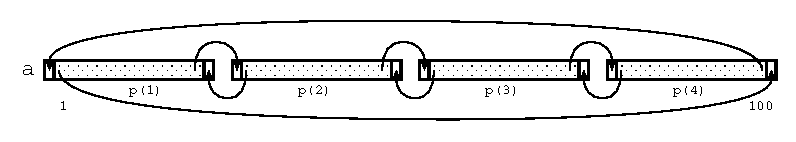
\includegraphics[width=0.9\hsize]{figs/fig3.2.eps}
\end{center}
\caption{Example of periodic shadow reflection.}
\label{fig3.2}
\end{myfigure}

The {\tt shadow} directive allocates ``periodic'' shadow areas of the
array {\tt a}.
The {\tt reflect} construct updates ``periodically'' the shadow area of
{\tt a} (Figure \ref{fig3.2}). A periodic shadow at the lower
bound on the node {\tt p(1)} is updated with the value of {\tt a(100)}
and that at the upper bound on {\tt p(4)} with the value of {\tt a(1)}.


\subsection{{\tt gmove} Construct}

\subsubsection*{Synopsis}

%The {\tt \Directive{gmove}} construct copies the data of a
%distributed array in the global view. 

The {\tt \Directive{gmove}} construct allows an assignment statement,
which may cause communication, to be executed possibly in parallel by
the executing nodes.

\subsubsection*{Syntax}
\Syntax{gmove}

\begin{tabular}{ll}
\verb![F]! & \verb|!$xmp| {\tt gmove} {\openb}{\tt in} $\vert$ {\tt
 out}{\closeb} {\openb}{\tt async (} {\it async-id} {\tt )}{\closeb}\\
% {\it dest} {\tt =} {\it source} \\
\verb![C]! & \verb|#pragma xmp| {\tt gmove} {\openb}{\tt in} $\vert$ {\tt
     out}{\closeb} {\openb}{\tt async (} {\it async-id} {\tt )}{\closeb}\\
% {\it dest} {\tt =} {\it source} \\
\end{tabular}

\subsubsection*{Description}

This construct copies the value of the right-hand side variable
into the left-hand side of the associated assignment statement,
which may cause communication between the executing nodes. Such
communication is detected, scheduled, and performed by the XcalableMP
runtime system.

%This construct executes a copy operation of the global data array object
%distributed into nodes.
%This directive is followed by the assignment
%statement of the scalar value and array sections.
%The assignment may require communication between nodes.

%Note that, in {\XMP}, the {\C} language is extended to support array
%section notation in order to support an assignment of array objects.

%The assignment statement must have one of the following patterns:
%
%\begin{itemize}
%\item  Scalar assignment. For example:
%
%\begin{tabular}{lll}
%\hspace{0.5cm} & {\tt s1 = s2} & ! {\tt s1} and {\tt s2} is a scalar
%variable \\ 
%& {\tt a(3) = b(i, j)} & ! {\tt a} and {\tt b} are arrays. \\
%\end{tabular}
%
%\item Array assignment. The left-hand-side variable must be either an
%      array name, an array section, or a scalar object. For example:
%
%\begin{tabular}{lll}
%\hspace{0.5cm} & {\tt a = b} & ! {\tt a} and {\tt b} are arrays \\
% & {\tt a(1:10) = b(n:n+9, k)} & ! left-hand side and right-hand side are array sections \\
% & {\tt a(1:10) = s2} & ! left-hand side is an array section and right-hand side is a
% scalar variable \\
% & {\tt a(1:10) = b(i, j)} & ! left-hand side is an array section and right-hand side is a
% scalar object \\
%\end{tabular}
%\end{itemize}

%The {\tt gmove} construct must be executed by all of the executing
%nodes. The value of scalar objects, the index value, and the range
%value of the array section in the assignment statement must be the same in
%every node executing this directive.

There are three operating modes of the {\tt gmove} construct:

\begin{itemize}
 \item {\bf collective mode}\index{collective mode (of {\tt gmove})}

       When neither the {\tt in} nor the {\tt out} clause is specified,
       the copy operation is performed collectively, and results in 
       implicit synchronization among the executing nodes.

       If the {\tt async} clause is not specified, then the construct is
       ``synchronous,'' and it is guaranteed that the left-hand side
       data can be read and overwritten, the right-hand side data can be
       overwritten, and all of 
       the operations of the construct on the executing nodes are
       completed when returning from the construct;
       otherwise, the construct is ``asynchronous,'' and it is not
       guaranteed that the operations are completed, until the
       associating {\tt wait\_async} construct (Section
       \ref{subsec:wait_async Construct}) is completed.

%In this case, all elements in both the source array and the target array
%must be distributed onto the executing node set.
%If the object on the right-hand side is a local
%object, then the value of the local object must be the same.
%
%In this case, the assignment is performed locally, where the object on
%the left-hand side is distributed.
%
%If the object on the left-hand side is a local object
%and the object on the right-hand side is global, then this operation
%performs broadcast operation.

 \item {\bf in mode}\index{in mode (of {\tt gmove})}

       When the {\tt in} clause is specified, the right-hand side data of the
       assignment, all or part of which may reside outside the
       executing node set, can be transferred from its owner nodes to
       the executing nodes by this construct.

       If the {\tt async} clause is not specified, then the construct is
       ``synchronous,'' and it is guaranteed that the left-hand side data
       can be read and overwritten, and that all of the operations of the
       construct on the owner nodes of the right-hand side and the executing nodes
       are completed when returning from the construct;
       otherwise, the construct is ``asynchronous,'' and it is not
       guaranteed that the operations are completed, until the
       associating {\tt wait\_async} construct (Section
       \ref{subsec:wait_async Construct}) is completed.

 \item {\bf out mode}\index{out mode (of {\tt gmove})}

       When the {\tt out} clause is specified, the left-hand side data of the
       assignment, all or part of which may reside outside the 
       executing node set, can be transferred from the executing nodes
       to its owner nodes by this construct.

       If the {\tt async} clause is not specified, then the construct is
       ``synchronous,'' and it is guaranteed that the right-hand side data
       can be overwritten, and that all of the operations of the construct on
       the owner nodes of the left-hand side and the executing nodes are
       completed when returning from the construct; otherwise, the
       construct is ``asynchronous,'' and it is not guaranteed that the
       operations are completed, until the associating {\tt wait\_async}
       construct (Section \ref{subsec:wait_async Construct}) is completed.

\end{itemize}

%Note that, in these cases, no synchronization is implied and it is not
%ensured that the copy operation is completed. Thus, if a synchronization
%between the executing nodes and the owner nodes is required, the
%programmer must specify it explicitly by using a {\tt barrier} construct
%or a pair of a {\tt post} and an {\tt wait} construct.

%When an {\tt in} clause is specified, then the node that owns the
%element of the object on the left-hand side obtains the data on the
%right-hand side by the remote copy (get) operation.
%Therefore, the object on the left-hand side must be distributed onto
%the executing node set.
%
%When an {\tt out} clause is specified, then the node that owns the element
%of the object on the right-hand side places the data on the left-hand
%side by the remote copy (put) operation.
%Therefore, the object on the
%right-hand side must be distributed onto the executing node set.

%If no option is specified, then the copy can be performed by two-side
%communication. In this case, the receiver side waits for the sender side,
%resulting in implicit synchronization. 

%If an {\tt in} or {\tt out} clause is specified, then the
%copy operation should be performed by one-side communication for remote
%memory access. Thus, no synchronization is implied. If
%synchronization between reader and writer is required, then the programmer
%must perform synchronization explicitly by a {\tt barrier} construct. If
%the reader and the writer do not belong to the same executing node set,
%then point-to-point synchronization by {\tt post-wait} directive can be used.

When the {\tt async} clause is specified, the statements following this
construct may be executed before the operation is complete.

\subsubsection*{Restrictions}

\begin{itemize}
 \item The {\tt gmove} construct must be followed by (i.e., associated
       with) a simple assignment statement that contains neither
       arithmetic operations nor function calls.
 \item The {\tt gmove} construct is global, which means that it must be
       executed by all nodes in the current executing node set, and each local
       variable referenced in the construct must have the same value.
 \item If the {\tt gmove} construct is in the {\it collective} mode, then
       all elements of the distributed arrays appearing on both the
       left-hand side and the right-hand side of the associated assignment
       statement must reside in the executing node set.
 \item If the {\tt gmove} construct is in the {\it in} mode, then
       all elements of the distributed array appearing on the left-hand side of the
       associated assignment statement must reside in the executing node
       set.
 \item If the {\tt gmove} construct is in the {\it out} mode, then
       all elements of the distributed array appearing on the right-hand side of the
       associated assignment statement must reside in the executing node
       set.
 \item {\it async-id} must be an expression of type default integer in
       {\XMPF} or type {\tt int} in {\XMPC}.
\end{itemize}

\subsubsection*{Examples}
\begin{description}
\item[Example 1: Array assignment]
\Example{gmove}

If the arrays on both the left-hand side and the right-hand side are distributed, then the copy
operation is performed using all-to-all 
communication. If the left-hand side is a replicated array, this copy
is performed using multi-cast communication. If the right-hand side is a
replicated array, then no communication is required.

\vspace{0.5cm}

\begin{minipage}{0.45\hsize}
\begin{center}
\begin{XFexample}
!$xmp gmove
      a(:,1:N) = b(:,3,0:N-1)
\end{XFexample}
\end{center}
\end{minipage}
\begin{minipage}{0.45\hsize}
\begin{center}
\begin{XCexampleR}
#pragma xmp gmove
      a[1:N][:] = b[0:N][3][:];
\end{XCexampleR}
\end{center}
\end{minipage}
\vspace{1cm}

\item[Example 2: Scalar assignment to an array] 

When the right-hand side is an element of a distributed array, the copy operation
is performed by broadcast communication from the owner of the element. If 
the right-hand side is a replicated array, then no communication is required.

\vspace{0.5cm}

\begin{minipage}{0.45\hsize}
\begin{center}
\begin{XFexample}
!$xmp gmove
      a(:,1:N) = c(k)
\end{XFexample}
\end{center}
\end{minipage}
\begin{minipage}{0.45\hsize}
\begin{center}
\begin{XCexampleR}
#pragma xmp gmove
      a[1:N][:] = c[k]
\end{XCexampleR}
\end{center}
\end{minipage}
\vspace{1cm}

\item[Example 3: in mode assignment]

	   Because {\tt b(3)} referenced on the right-hand side of the
	   {\tt gmove} construct does not reside in the executing node
	   set ({\tt p(1:2)}), the construct is executed in the {\it in}
	   mode. Thus, {\tt b(3)} is transferred from its owner node
	   {\tt p(3)} to the executing node set.

	   Until {\tt p(1:2)} returns from the
	   construct, there is no gurantee that any node can read and
	   overwrite {\tt a(1:2)},
	   and that any relevant operations on {\tt p(1:2)} and {\tt p(3)}
	   are completed.

\vspace{0.5cm}

\begin{XFexample}
!$xmp nodes p(4)
!$xmp template t(4)
!$xmp distribute t(block) onto p

      real a(4), b(4)
!$xmp align (i) with t(i) : a, b
      ...
!$xmp task on p(1:2)
      ...
!$xmp gmove in
      a(1:2) = b(2:3)
      ...
!$xmp end task
\end{XFexample}

%$

\end{description}

\subsection{{\tt barrier} Construct}

\subsubsection*{Synopsis}

The {\tt \Directive{barrier}} construct specifies an explicit barrier
at the point at which the construct appears. 

\subsubsection*{Syntax}
\Syntax{barrier}

\begin{tabular}{ll}
\verb![F]! & \verb|!$xmp| {\tt barrier} {\openb}{\tt on} {\it nodes-ref}
 $\vert${\it template-ref}{\closeb} \\
\verb![C]! & \verb|#pragma xmp| {\tt barrier} {\openb}{\tt on} {\it
     nodes-ref} $\vert$ {\it template-ref}{\closeb} \\
\end{tabular}

\subsubsection*{Description}

The barrier operation is performed among the node set specified by
the {\tt on} clause. If no {\tt on} clause is specified, then it is
assumed that the current executing node set is specified in it.

Note that an {\tt on} clause may represent multiple node sets. In such a
case, a barrier operation is performed in each node set.

%The barrier construct also has the function of ensuring that all of the
%remote copy operations that are invoked by gmove in/out constructs
%executed by the node set specified by the {\tt on} clause are finished.

\subsubsection*{Restriction}

\begin{itemize}
\item The node set specified by the {\tt on} clause must be a subset of the
      executing node set.  
\end{itemize}


\subsection{{\tt reduction} Construct}

\subsubsection*{Synopsis}

The {\tt \Directive{reduction}} construct performs a reduction
operation among nodes. 

\subsubsection*{Syntax}
\Syntax{reduction}

\begin{tabular}{ll}
\verb![F]! & \verb|!$xmp| {\tt reduction (} {\it reduction-kind} {\it
  :} {\it variable} {\openb}, {\it variable} {\closeb}... {\tt )}
 {\bsquare} \\
 & \hspace{6cm} {\bsquare} {\openb}{\tt on} {\it node-ref} $\vert$ {\it
     template-ref}{\closeb} {\openb}{\tt async (} {\it async-id} {\tt
     )}{\closeb} \\
\end{tabular}

\vspace{0.5cm}

where {\it reduction-kind} is one of:

\begin{tabular}{ll}
 \hspace{0.5cm} & {\tt +} \\
 & {\tt *} \\
% & {\tt -} \\
 & {\tt .and.} \\
 & {\tt .or.} \\
 & {\tt .eqv.} \\
 & {\tt .neqv.} \\
 & {\tt max} \\
 & {\tt min} \\
 & {\tt iand} \\
 & {\tt ior} \\
 & {\tt ieor} \\
\end{tabular}

\vspace{0.5cm}

\begin{tabular}{ll}
 \hspace{-\parindent}
 \verb![C]! & \verb|#pragma xmp| {\tt reduction (} {\it reduction-kind} {\it
  :} {\it variable} {\openb}, {\it variable} {\closeb}... {\tt )}
 {\bsquare} \\
 & \hspace{6cm} {\bsquare} {\openb}{\tt on} {\it node-ref} $\vert$ {\it
     template-ref}{\closeb} {\openb}{\tt async (} {\it async-id} {\tt
     )}{\closeb} \\
\end{tabular}

\vspace{0.5cm}

where {\it reduction-kind} is one of:

\begin{tabular}{ll}
 \hspace{0.5cm} & {\tt +} \\
 & {\tt *} \\
% & {\tt -} \\
 & {\verb|&|} \\
 & {\tt |} \\
 & {\verb|^|} \\
 & {\verb|&&|} \\
 & {\tt ||} \\
 & {\tt max} \\
 & {\tt min} \\
\end{tabular}

\subsubsection*{Description}

The {\tt reduction} construct performs a type of
% modified by Sakagami,H. 09/11/13                                            
reduction operation specified by {\it reduction-kind} for the specified
local variables among the node set specified by the {\tt on}
clause, and it sets the reduction results to the variables on each of the
nodes.
%
Note that some of the reduction operations, namely, {\tt FIRSTMAX}, {\tt
FIRSTMIN}, {\tt LASTMAX}, and {\tt LASTMIN}, which can be specified in
the {\tt reduction} clause of the {\tt loop} directive, cannot be
specified in the {\tt reduction} construct because their semantics are
not defined for it.
%
The variable specified by {\it variable}, which is the target of the
reduction operation, is referred to as the ``\Term{reduction
variable}.'' After the reduction operation, the value of a reduction
variable becomes the same in every node that performs the operation.

The reduction result is computed by combining the reduction variables on
all of the nodes using the reduction operator. The ordering of this
reduction is unspecified.

When the {\tt async} clause is specified, the statements following this
construct may be executed before the operation is complete.

% inserted by Sakagami,H. 09/11/13 ----- start ----                            
When {\it template-ref} is specified in the {\tt on} clause, the operation
is performed in a node set that consists of nodes onto which the
specified template section is distributed.
Therefore, before the {\tt reduction} construct is executed, the
referenced template must be fixed.
%
%When {\it template-subscript} in the {\it template-ref} is ``*'', nodes
%in the corresponding dimension are ignored for the reduction operation.
%
%When {\it template-subscript} in the {\it template-ref} is {\it
%triplet}, nodes for all template elements in the corresponding dimension
%perform the reduction operation.
%
When {\it nodes-ref} is specified in the {\tt on} clause, the operation
is performed in the specified node set.
%Therefore, before the {\tt \Directive{reduction}} construct is executed,
%the referenced node set must be fixed.
%
When the {\tt on} clause is omitted, the operation is performed in the
executing node set.

Note that an {\tt on} clause may represent multiple node sets. In such a
case, a reduction operation is performed in each node set.

\subsubsection*{Restrictions}

\begin{itemize}
%\item {\it template-spec} appearing in {\it template-ref} must be either ``*'', ``\
%:'' or the range.
%\item If {\tt on} clause is omitted, the operation is done in the current execu\
%ting node.
 \item The variables specified by the sequence of {\it variables} must
       either not be aligned or must be replicated among nodes of the node
       set specified by the {\tt on} clause.
 \item The {\tt reduction} construct is global, which means that it must
       be executed by all nodes in the current executing node set, and each local
       variable referenced in the construct must have the same value.
 \item {\it async-id} must be an expression of type default integer in
       {\XMPF} or type {\tt int} in {\XMPC}.
 \item The node set specified by the {\tt on} clause must be a subset of the
       executing node set.
\end{itemize}
% inserted by Sakagami,H. 09/11/13 ----- end ---- 

\subsubsection*{Examples}
\Example{reduction}

\begin{description}
\item[Example 1]
\hspace{\hsize}
\begin{XFexample}
!$xmp reduction(+:s)
!$xmp reduction(max:aa) on t(*,:)
!$xmp reduction(min:bb) on p(10:30)
\end{XFexample}

% modified by Sakagami,H. 09/11/13                                             
%In the first example, the scalar variable {\tt s} is assumed to contain the 
%partial sum of the variable, and the reduction operation calculates the
%total sum of the variable. The total sum is stored in the variable in
%each node.
In the first line, the reduction operation calculates the sum of the
scalar variable {\tt s} in the executing node set, and the result is
stored in the variable in each node.

% modified by Sakagami,H. 09/11/13                                             
The reduction operation in the second line computes the maximum value of
the variable {\tt aa} in each node set onto which each of the template
sections specified by {\tt t(*,:)} is distributed.
%that consists of nodes associated with the
%range of the second dimension of template {\tt t}.

% modified by Sakagami,H. 09/11/13                
In the third line, the minimum value of the variable {\tt bb} in the node 
set specified by {\tt p(10:30)} is calculated. This example is
equivalent to the following code using the {\tt task} construct.

\begin{XFexample}
!$xmp task on p(10:30)
!$xmp reduction(min:bb)
!$xmp end task
\end{XFexample}

\item[Example 2]
\hspace{\hsize}
\begin{XFexample}
      dimension a(n,n), p(n), w(n)
!$xmp align a(i,j) with t(i,j)
!$xmp align p(i) with t(i,*)
!$xmp align w(j) with t(*,j)
      ...
!$xmp loop (j) on t(:,j)
      do j = 1, n
          sum = 0
!$xmp loop (i) on t(i,j) reduction(+:sum)
          do i = 1, n
              sum = sum + a(i,j) * p(i)
          end do
          w(j) = sum
      end do
\end{XFexample}

This code computes the matrix vector product,
% modified by Sakagami,H. 09/11/13
where a {\tt reduction} clause is specified for the {\tt \Directive{loop}}
construct of the inner loop. This is equivalent to the following code
snippet. 

\begin{XFexample}
!$xmp loop (j) on t(:,j)
      do j = 1, n
          sum = 0
!$xmp loop (i) on t(i,j) 
          do i = 1, n
              sum = sum + a(i,j) * p(i)
          end do
!$xmp reduction(+:sum) on t(1:n,j)
          w(j) = sum
      end do
\end{XFexample}

In these cases, the reduction operation on the scalar variable {\tt sum}
is performed for every iteration in the outer loop, which may cause a
large overhead.
% modified by Sakagami,H. 09/11/13
To reduce this overhead, the {\tt reduction} clause should be specified
in the {\tt \Directive{loop}} construct for the outer loop.
%
%because the loop index of the outer loop ({\tt j}) is different from that 
%for the reduction operation ({\tt i}).
This is because the node set in which the reduction operation is
performed is determined on the basis of its {\tt on} clause (see
\ref{sub:loop_construct}), and the {\tt on} clause of the outer {\tt
loop} construct is different from that of the inner one. 
%
However, this code can be modified using the {\tt reduction}
construct as follows: 

\begin{XFexample}
      dimension a(n,n), p(n), w(n)
!$xmp align a(i,j) with t(i,j)
!$xmp align p(i) with t(i,*)
!$xmp align w(j) with t(*,j)
      ...
!$xmp loop (j) on t(:,j)
      do j = 1, n
          sum = 0
!$xmp loop (i) on t(i,j) 
          do i = 1, n
              sum = sum + a(i,j) * p(i)
          end do
          w(j) = sum
      end do
!$xmp reduction(+:w) on t(1:n,*)
\end{XFexample}

This code performs a reduction operation on the array {\tt w} only once,
which may result in faster operation.  

\end{description}


\subsection{{\tt bcast} Construct}

\subsubsection*{Synopsis}

The {\tt \Directive{bcast}} construct performs broadcast communication
from a specified node.

\subsubsection*{Syntax}
\Syntax{bcast}

\begin{tabular}{ll}
 \verb![F]! & \verb|!$xmp| {\tt bcast} \verb|(| {\it variable} 
 {\openb}, {\it variable}{\closeb}... \verb|)|
 {\openb}{\tt from} {\it nodes-ref} $\vert$ {\it template-ref}{\closeb}
 {\bsquare} \\
 & \hspace{5cm} {\bsquare} {\openb}{\tt on} {\it nodes-ref}{\closeb}
     $\vert$ {\it template-ref}{\closeb}
     {\openb}{\tt async (} {\it async-id} {\tt )}{\closeb} \\

 \verb![C]! & \verb|#pragma xmp| {\tt bcast} \verb|(| {\it variable} 
 {\openb}, {\it variable}{\closeb}... \verb|)|
 {\openb}{\tt from} {\it nodes-ref}  $\vert$ {\it
     template-ref}{\closeb} {\bsquare} \\
 & \hspace{5cm} {\bsquare} {\openb}{\tt on} {\it nodes-ref} $\vert$ {\it
     template-ref}{\closeb}
 {\openb}{\tt async (} {\it async-id} {\tt )}{\closeb} \\

\end{tabular}

\subsubsection*{Description}

The values of the variables specified by the sequence of {\it
variables} (called {\it \Term{broadcast variables}}) are broadcasted 
from the node specified by the {\tt from} clause (called the
{\it \Term{source node}}) to each of the nodes in the node set specified
by the {\tt on} clause. After executing this construct,
the values of the broadcast variables become the same as those in the
source node.
%
If the {\tt from} clause is omitted, then the {\it first}
node, that is, the leading one in Fortran's array element order, of the
node set specified by the {\tt on} clause is assumed to be a source
node.
%
If the {\tt on} clause is omitted, then it is assumed that the current
executing node set is specified in it.

When the {\tt async} clause is specified, the statements following this
construct may be executed before the operation is complete.

\subsubsection*{Restrictions}

\begin{itemize}
 \item The variables specified by the sequence of {\it variables} must
       either not be aligned or must be replicated among nodes of the node set
       specified by the {\tt on} clause.
 \item The {\tt bcast} construct is global, which means that it must be
       executed by all nodes in the current executing node set, and each local
       variable referenced in the construct must have the same value
       among all of them.
 \item {\it async-id} must be an expression of type default integer in
       {\XMPF} or type {\tt int} in {\XMPC}.
 \item The node set specified by the {\tt on} clause must be a subset of
       the executing node set.
 \item The source node specified by the {\tt from} clause must belong to
       the node set specified by the {\tt on} clause.
 \item The source node specified by the {\tt from} clause must be one node.
\end{itemize}


\subsection{{\tt wait\_async} Construct}
\label{subsec:wait_async Construct}

\subsubsection*{Synopsis}

The {\tt \Directive{wait\_async}} construct guarantees that asynchronous
communications specified by {\it async-id} are complete.

\subsubsection*{Syntax}
\Syntax{wait\_async}

\begin{tabular}{ll}
\verb![F]! & \verb|!$xmp| {\tt wait\_async ( {\it async-id} {\openb},
 {\it async-id} {\closeb}... )} {\openb}{\tt on} {\it nodes-ref} $\vert$
 {\it template-ref}{\closeb} \\
\verb![C]! & \verb|#pragma xmp| {\tt wait\_async ( {\it async-id} {\openb},
 {\it async-id} {\closeb}... )} {\openb}{\tt on} {\it nodes-ref} $\vert$
 {\it template-ref}{\closeb}\\
\end{tabular}

\subsubsection*{Description}

The {\tt \Directive{wait\_async}} construct will block, and therefore
statements following it will not be executed, until the completion of
all of 
the asynchronous communications that are specified by {\it async-id}'s
and issued on the node set specified by the {\tt on} clause.
\mytextcolor{red}{
If an {\it async-id} is not associated with any asynchronous
communication, the {\tt wait\_async} construct ignores it.
}

\subsubsection*{Restrictions}

\begin{itemize}
 \item {\it async-id} must be an expression of type default integer in
       {\XMPF} or type {\tt int} in {\XMPC}.
 \item \mytextcolor{red}{\sout{{\it async-id} must be associated with an asynchronous
       communication using the {\tt async} clause of a communication
       construct.}}
 \item The {\tt wait\_async} construct is global, which means that it must
       be executed by all nodes in the current executing node set, and
       each local variable referenced in the construct must have the
       same value among all of them.
 \item The node set specified by the {\tt on} clause must be the same as
       those of the global constructs that initiate the asynchronous
       communications specified by {\it async-id}.
%\item Every communication specified by each {\it async-id} must be
%      executed on the same executing node set.
\end{itemize}


\subsection{{\tt async} Clause}
\index{async clause@{\tt async} clause}
\index{Directive!async clause@{{\tt async} clause}}

\subsubsection*{Synopsis}

The {\tt async} clause of the {\tt reflect}, {\tt gmove}, {\tt
reduction}, and {\tt bcast} constructs enables the corresponding
communication to be performed asynchronously.

\subsubsection*{Description}

Communication corresponding to the construct with an {\tt async} clause
is performed asynchronously, that is, it is initiated but not completed,
and therefore, statements following it may be executed before the
communication is complete.

%\subsubsection*{Restrictions}
%
%\begin{itemize}
% \item A node must not issue at runtime an asynchronous communication
%       with an {\tt async-id} until every other one with the same {\tt
%       async-id} is complete.
%\end{itemize}

\subsubsection*{Example}
\Example{async}
\Example{wait\_async}

\begin{XFexample}
!$xmp reflect (a) async(1)
      S1
!$xmp wait_async(1)
      S2
\end{XFexample}

The {\tt reflect} construct on the first line matches the {\tt wait}
construct on the third line because both of their {\it async\_id}
evaluate to one.
%
These constructs ensure that statements in {\tt S1} can be executed
before the {\tt reflect} communication is complete, and no statement in
{\tt S2} is executed until the {\tt reflect} communication is
complete.


\mytextcolor{red}{
\subsection{{\tt reduce\_shadow} Construct}
\label{154624_16Jan17}
}

\subsubsection*{Synopsis}

The {\tt \Directive{reduce\_shadow}} construct adds values of shadow
objects to their reflection source.

\subsubsection*{Syntax}
\Syntax{reduce\_shadow}

\begin{tabular}{ll}
 \verb![F]! & \verb|!$xmp| {\tt reduce\_shadow} \verb|(| {\it array-name}
 {\openb}, {\it array-name}{\closeb}... \verb|)| {\bsquare} \\
 &\hspace{0.3cm} {\bsquare} {\openb}{\tt width (} {\it reflect-width}
     {\openb}, {\it reflect-width}{\closeb}... {\tt )}{\closeb}
     {\openb}{\tt orthogonal}{\closeb}
     {\openb}{\tt async (} {\it async-id} {\tt )}{\closeb} \\
\verb![C]! & \verb|#pragma xmp| {\tt reduce\_shadow} \verb|(| {\it array-name}
     {\openb}, {\it array-name}{\closeb}... \verb|)| {\bsquare} \\
 &\hspace{0.3cm} {\bsquare} {\openb}{\tt width (} {\it reflect-width}
     {\openb}, {\it reflect-width}{\closeb}... {\tt )}{\closeb}
     {\openb}{\tt orthogonal}{\closeb}
     {\openb}{\tt async (} {\it async-id} {\tt )}{\closeb} \\
\end{tabular}

\subsubsection*{Description}

The {\tt reduce\_shadow} construct adds values of shadow objects of the
array specified by {\it array-name} to their reflection source. Note
that the shadow objects corresponding to elements at the non-orthogonal
positions are also added as the default behavior.

When the {\tt width} clause is specified and has the form ``{\it
int-expr} : {\it int-expr}'' in a dimension, the shadow areas having the
width specified by the first {\it int-expr} at the lower bound, and that
specified by the second one at the upper bound in the dimension are
added.
%
When the {\tt width} clause is specified and has the form {\it int-expr},
the shadow areas having the same width specified at both the upper
and lower bounds in the dimension are added.
%
When the {\tt width} clause is omitted, the whole shadow area of the array
is added.

In particular, when the \Term{{\tt /periodic/} modifier} is specified in
{\it reflect-width}, the addition of the shadow object in the dimension is
``periodic,'' which means that the shadow object at the global lower
(upper) bound is treated as if it corresponds to the data object of the
global upper (lower) bound and is added by the {\tt reduce\_shadow}
construct.

When the {\tt orthogonal} clause is specified,
the shadow object is added only by orthogonal nodes.

When the {\tt async} clause is specified, the statements following this
construct may be executed before the operation is complete.

\subsubsection*{Restrictions}

\begin{itemize}
 \item The arrays specified by the sequence of {\it array-names} must
       be mapped onto the executing node set.
 \item The width of each dimension specified by {\it
       reflect-width} must not exceed the shadow width of the arrays.
 \item The {\tt reduce\_shadow} construct is global, which means that it must be
       executed by all nodes in the current executing node set, and each local
       variable referenced in the construct must have the same value
       among all of them.
 \item {\it async-id} must be an expression of type default integer in
       {\XMPF} or type {\tt int} in {\XMPC}.
\end{itemize}

\subsubsection*{Examples}
\Example{reduce\_shadow}

\begin{XFexample}
      real rho(n,n)
!$xmp align rho(i,j) with t1(i,j)
!$xmp shadow rho(1:1)

      real f(m)
      integer x(m), y(m)
!$xmp align (k) with t2(k) : f, x, y

!$xmp loop on t2(k)
      do i = 1, no
        ix = x(i)
        iy = y(i)
        dx = x(i) - ix
        dy = y(i) - iy
        rho(ix  ,iy  ) = rho(ix  ,iy  ) + (1.0-dx)*(1.0-dy)*f(i)
        rho(ix+1,iy  ) = rho(ix+1,iy  ) +      dx *(1.0-dy)*f(i)
        rho(ix  ,iy+1) = rho(ix  ,iy+1) + (1.0-dx)*     dy *f(i)
        rho(ix+1,iy+1) = rho(ix+1,iy+1) +      dx *     dy *f(i)
      end do

!$xmp reduce_shadow (rho)
!$xmp reflect (rho)
\end{XFexample}

Assume that a two-dimensional field {\tt rho} and m particles are
both distributed onto nodes. On each node, a contribution of a particle
{\tt f(k)} is added to the nearest grid point of the field and its
neighbors, which may be in the shadow area on the node. In the last two
lines, the values of the shadow area from neighboring nodes are added to
the corresponding data object, and the results are then copied back to
the shadow area on the neighboring nodes.

\cleardoublepage

\chapter{Intrinsic and Library Procedures}
\label{chap:Intrinsic and library procedures}

This specification defines various procedures for system inquiry,
synchronization, computations, etc. The procedures are provided as
intrinsic procedures in {\XMPF} and library procedures in {\XMPC}.

\section{System Inquiry Procedures}

\begin{itemize}
 \item {\tt xmp\_desc\_of}
 \item {\tt xmp\_all\_node\_num}
 \item {\tt xmp\_all\_num\_nodes}
 \item {\tt xmp\_node\_num}
 \item {\tt xmp\_num\_nodes}
% \item {\tt xmp\_mpi\_comm}
 \item {\tt xmp\_wtime}
 \item {\tt xmp\_wtick}
\end{itemize}

\subsection{\tt xmp\_desc\_of}
\label{subsec: xmp_desc_of}
\Intrinsic{xmp\_desc\_of}
\index{descriptor-of operator}
\index{xmp\_desc\_of@{\tt xmp\_desc\_of}}

\subsubsection*{Format}

\begin{tabular}{lll}

\verb![F]!&  {\tt integer(kind=xmp\_desc\_kind)}& {\tt xmp\_desc\_of(xmp\_entity)}\\

\verb![C]!&  {\tt xmp\_desc\_t}& {\tt xmp\_desc\_of(xmp\_entity)}

\end{tabular}

\vspace{0.3cm}

Note that {\tt xmp\_desc\_of} is an intrinsic function in {\XMPF} or
a built-in operator in {\XMPC}.

\subsubsection*{Synopsis}

%    A {\tt xmp\_desc\_of} is an input argument of query functions.
%    When Query functions get descriptor information of array
%    from XMP compiler, they must set a {\tt xmp\_desc\_of} as an
%    input argument.

{\tt xmp\_desc\_of} returns, in {\XMPF}, or is evaluated to, in {\XMPC},
a descriptor to retrieve informations of the specified global array,
template, or node array. The resulting descriptor can be used as an
input argument of the inquiry procedures which is described in appendix
\ref{chap:Interface to Numerical Libraries}.

The kind type parameter of the type of the descriptor, {\tt
xmp\_desc\_kind}, in {\XMPF} is implementation-dependent, and defined in
a Fortran module named {\tt xmp\_lib} or a Fortran {\tt include} file
named {\tt xmp\_lib.h}.

The type of the descriptor, {\tt xmp\_desc\_t}, in {\XMPC} is
implementation-dependent, and defined in a header file named {\tt xmp.h}
in {\XMPC}.

%The type of the descriptor, {\tt xmp\_desc\_t}, is
%implementation-dependent, and defined in a Fortran module named {\tt
%xmp\_lib} or a Fortran {\tt include} file named {\tt xmp\_lib.h} in
%{\XMPF}, or a header file named {\tt xmp.h} in {\XMPC}.

\subsubsection*{Arguments}

The argument or operand {\tt xmp\_entity} is the name of either a global
array, a template or a node array.

%   The argument of {\tt xmp\_desc\_of} is an {\it array-name}, a {\it template-name}, or a {\it nodes-name}.
%   In the case of {\it array-name}, return value d is a pointer to
%   be able to access array descriptor information.
%   In the case of {\it template-name}, return value d is a pointer to
%   be able to access template descriptor information.
%   In the case of {\it nodes-name}, return value d is a pointer to
%   be able to access node descriptor information.
%   If the argument of {\tt xmp\_desc\_of} is a local data, it is unchanged.


\subsection{\tt xmp\_all\_node\_num}
\Intrinsic{xmp\_all\_node\_num}

\subsubsection*{Format}

\begin{tabular}{lll}

\verb![F]!&  {\tt integer function}& {\tt xmp\_all\_node\_num()}\\

\verb![C]!&  {\tt int}& {\tt xmp\_all\_node\_num(void)}

\end{tabular}

\subsubsection*{Synopsis}

     The {\tt xmp\_all\_node\_num} routine returns the node number,
     within the primary node set, of the node that calls {\tt
     xmp\_all\_node\_num}.

\subsubsection*{Arguments}

    none.


\subsection{\tt xmp\_all\_num\_nodes}
\Intrinsic{xmp\_all\_num\_nodes}

\subsubsection*{Format}

\begin{tabular}{lll}

\verb![F]!&  {\tt integer function}& {\tt xmp\_all\_num\_nodes()}\\

\verb![C]!&  {\tt int}& {\tt xmp\_all\_num\_nodes(void)}

\end{tabular}

\subsubsection*{Synopsis}

     The {\tt xmp\_all\_num\_nodes} routine returns the number of nodes
     in the entire node set.

\subsubsection*{Arguments}

    none.


\subsection{\tt xmp\_node\_num}
\Intrinsic{xmp\_node\_num}

\subsubsection*{Format}

\begin{tabular}{lll}

\verb![F]!&  {\tt integer function}& {\tt xmp\_node\_num()}\\

\verb![C]!&  {\tt int}& {\tt xmp\_node\_num(void)}

\end{tabular}

\subsubsection*{Synopsis}

     The {\tt xmp\_node\_num} routine returns the node number,
     within the current executing node set, of the node that calls {\tt
     xmp\_node\_num}.

\subsubsection*{Arguments}

none.


\subsection{\tt xmp\_num\_nodes}
\Intrinsic{xmp\_num\_nodes}

\subsubsection*{Format}

\begin{tabular}{lll}

\verb![F]!&  {\tt integer function}& {\tt xmp\_num\_nodes()}\\

\verb![C]!&  {\tt int}& {\tt xmp\_num\_nodes(void)}

\end{tabular}

\subsubsection*{Synopsis}

     The {\tt xmp\_num\_nodes} routine returns the number of the
     executing nodes.

\subsubsection*{Arguments}

none.

%\subsection{\tt xmp\_mpi\_comm}
%
%\subsubsection*{Format}
%
%\begin{tabular}{lll}
%
%\verb![F]!&  {\tt integer function}& {\tt xmp\_mpi\_comm({\it nodes-name})}\\
%
%\verb![C]!&  {\tt int}& {\tt xmp\_mpi\_comm({\it nodes-name})}
%
%\end{tabular}
%
%\subsubsection*{Synopsis}
%     The {\tt xmp\_mpi\_comm} routine returns the integer value with associated communicator
%     to which {\it nodes-name} belongs. If non {\it nodes-name}, {\tt xmp\_mpi\_comm} returns 
%     the value of MPI\_Comm\_World.
%
%\subsubsection*{Arguments}
%    The argument of {\tt xmp\_mpi\_comm} is a {\it nodes-name} of the executing node set.
%
%

\subsection{\tt xmp\_wtime}
\Intrinsic{xmp\_wtime}

\subsubsection*{Format}

\begin{tabular}{lll}

\verb![F]!&  {\tt double precision function}& {\tt xmp\_wtime()}\\

\verb![C]!&  {\tt double}& {\tt xmp\_wtime(void)}

\end{tabular}

\subsubsection*{Synopsis}
    The {\tt xmp\_wtime} routine returns elapsed wall clock time in seconds 
    since some time in the past. The ``time in the past'' is guaranteed
    not to change during the life of the process.
    There is no requirement that different nodes return ``the same time.''

\subsubsection*{Arguments}
    none.


\subsection{\tt xmp\_wtick}
\Intrinsic{xmp\_wtick}

\subsubsection*{Format}

\begin{tabular}{lll}

\verb![F]!&  {\tt double precision function}& {\tt xmp\_wtick()}\\

\verb![C]!&  {\tt double}& {\tt xmp\_wtick(void)}

\end{tabular}

\subsubsection*{Synopsis}
    The {\tt xmp\_wtick} routine returns the resolution of the timer
    used by {\tt xmp\_wtime}. 
    It returns a double precision value equal to the number of seconds 
    between successive clock ticks.

\subsubsection*{Arguments}
    none.


%\subsection{\tt xmp\_barrier}
%
%\subsubsection*{Format}
%
%\begin{tabular}{lll}
%
%\verb![F]!&  & {\tt xmp\_barrier({\it nodes-name})}\\
%
%\verb![C]!&  {\tt void}& {\tt  xmp\_barrier({\it nodes-name})}
%
%\end{tabular}
%
%\subsubsection*{Synopsis}
%    The {\tt xmp\_barrier} routine blocks the caller until all nodes in the executing node set 
%    indicated by {\it nodes-name} have called it.
%    The call returns at any process only after all {\it nodes-name} member's nodes
%    have entered the call.
%
%\subsubsection*{Arguments}
%    The argument of {\tt xmp\_barrier} is a {\it nodes-name} of the executing node set.
%

%\section{Computational Intrinsic Procedures}
%
%\subsection{Fortran}
%
%\begin{itemize}
% \item {\tt x = xmp\_scatter(a, idx1, idx2, ...)}
% \item {\tt x = xmp\_gather(a, idx1, idx2, ...)}
% \item {\tt v = xmp\_pack(a, mask)}
% \item {\tt a = xmp\_unpack(v, mask)}
% \item {\tt x = xmp\_sort\_up(a)}
% \item {\tt x = xmp\_sort\_down(a)}
% \item {\tt x = xmp\_cshift(a, shift, dim)}
% \item {\tt x = xmp\_eoshift(a, shift, b, dim)}
% \item {\tt m = xmp\_transpose(m)}
%\end{itemize}
%
%
%\subsection{C}
%
%
%\begin{itemize}
% \item {\tt x = xmp\_scatter(desc\_a, idx1, idx2, ...)}
% \item {\tt x = xmp\_gather(desc\_a, idx1, idx2, ...)}
% \item {\tt v = xmp\_pack(desc\_a, mask)}
% \item {\tt a = xmp\_unpack(desc\_v, mask)}
% \item {\tt x = xmp\_sort\_up(desc\_a)}
% \item {\tt x = xmp\_sort\_down(desc\_a)}
% \item {\tt x = xmp\_cshift(desc\_a, shift, dim)}
% \item {\tt x = xmp\_eoshift(desc\_a, shift, b, dim)}
% \item {\tt m = xmp\_transpose(desc\_m)}
%\end{itemize}


\section{Synchronization Procedures}

\subsection{\tt xmp\_test\_async}
\Intrinsic{xmp\_test\_async}

\begin{tabular}{lll}

\verb![F]!& {\tt logical function} & {\tt xmp\_test\_async(async\_id)}\\
          & {\tt integer} & {\tt async\_id}\\
          & & \\
\verb![C]!&  {\tt int} & {\tt  xmp\_test\_async(int async\_id)}

\end{tabular}

\subsubsection*{Synopsis}

The {\tt xmp\_test\_async} routine returns {\tt .true.}, in {\XMPF}, or
{\tt 1}, in {\XMPC}, if an asynchronous communication specified by the
argument {\tt async\_id} is complete; otherwise, it returns {\tt .false.}
or {\tt 0}.

\subsubsection*{Arguments}

The argument {\tt async\_id} is an integer expression that specifies an
asynchronous communication initiated by a global communication construct
with the {\tt async} clause.


\section{Miscellaneous Procedures}

\subsection{\tt xmp\_gtol}
\Intrinsic{xmp\_gtol}

\begin{tabular}{lll}

\verb![F]!& {\tt subroutine} & {\tt xmp\_gtol(d, g\_idx, l\_idx)} \\
          & {\tt integer(kind=xmp\_desc\_kind)} & {\tt d}\\
          & {\tt integer} & {\tt g\_idx(NDIMS)}\\
          & {\tt integer} & {\tt l\_idx(NDIMS)}\\
          & & \\
\verb![C]!&  {\tt void} & {\tt xmp\_gtol(xmp\_desc\_t d, int g\_idx[], int l\_idx[])}

\end{tabular}

\subsubsection*{Synopsis}

The {\tt xmp\_gtol} routine translates an index (specified by
{\tt g\_idx}) of a global array (specified by {\tt d}) into the
corresponding index of its local section and sets to an array specified
by {\tt l\_idx}. If the element of the specified index does not reside
in the caller of the routine, the resulting array is set to an
unspecified value.

\subsubsection*{Arguments}

\begin{itemize}
 \item {\tt d} is a descriptor, that is, an object of type {\tt
       integer(kind=xmp\_desc\_kind)}, in {\XMP}, or {\tt xmp\_desc\_t},
       in {\XMPC}, that is associated with the target global array.
 \item \verb![F]! {\tt g\_idx} is a rank-one integer array of the size
       equal to the rank of the target global array specified by {\tt
       d}.
 \item \verb![F]! {\tt l\_idx} is a rank-one integer array of the size
       equal to the rank of the target global array specified by {\tt
       d}.
 \item \verb![C]! {\tt g\_idx} is a one-dimensional integer array.
 \item \verb![C]! {\tt l\_idx} is a one-dimensional integer array.
\end{itemize}


\subsection{\tt [C] xmp\_malloc}
\label{subsec: xmp_malloc}
\Intrinsic{xmp\_malloc}

\begin{tabular}{ll}

{\tt void*} & {\tt xmp\_malloc(xmp\_desc\_t d, size\_t size)}

\end{tabular}

\subsubsection*{Synopsis}

The {\tt xmp\_malloc} routine allocates a storage for the local section
of a one-dimensional global array of size {\tt size} that is associated
with a descriptor specified by {\tt d}, and returns the pointer to it on
each node.

\subsubsection*{Arguments}

\begin{itemize}
 \item {\tt d} is a descriptor, that is, an object of type {\tt
       xmp\_desc\_t} that is associated with a pointer to the
       one-dimensional global array to be allocated.
 \item {\tt size} is the size of the global array to be allocated.
\end{itemize}

\cleardoublepage

\chapter{OpenMP in {\XMP} Programs}
\label{chap:openmp}

The usage of OpenMP directives in {\XMP} programs is subjected to
the following basic rule.

\begin{itemize}
 \item {\XMP} directives and the invocation of an {\XMP}
       intrinsic/built-in procedure should be single-threaded, and
       therefore may be placed in the sequential part, or one of
       the {\tt single}, {\tt master}, and {\tt critical} regions
       that is closely nested inside a {\tt parallel} region whose
       parent thread is the initial thread;

 \item with the exception that {\XMP}'s {\tt loop} directive that
       controls a loop can be placed immediately inside OpenMP's
       parallel loop directive ({\tt parallel do} for Fortran and
       {\tt parallel for} for C), which controls the identical loop.
\end{itemize}

The behavior of coarray references in a {\tt parallel} region is
implementation-dependent.

\subsubsection*{Examples}
\index{Example!OpenMP in XcalableMP programs}

Assume that the following codes are placed in the sequential part of
the program.

\begin{XCexample}
#pragma omp parallel for 
for (...){
  #pragma xmp barrier  // NG because not single-threaded
}
\end{XCexample}

\begin{XCexample}
#pragma omp parallel for 
for (...){
  #pragma omp single 
  {
    #pragma xmp barrier  // OK because single-threaded
                         // (inside a single region)
  }
}
\end{XCexample}

\begin{XCexample}
#pragma omp parallel for
#pragma xmp loop  // OK because immediately nested
for (...){
  ...
}
\end{XCexample}

\begin{XCexample}
#pragma xmp loop  // OK because single-threaded (not nested)
#pragma omp parallel for
for (...){
  ...
}
\end{XCexample}

\begin{XCexample}
#pragma xmp loop  // OK because single threaded (not nested)
for (...){
  #pragma omp parallel for
  for (...) { ... }
}
\end{XCexample}

\begin{XCexample}
#pragma omp parallel for 
for (...){
  #pragma xmp loop  // NG because not immediately nested
  for (...) { ... }
}
\end{XCexample}

\cleardoublepage

\chapter{Intrinsic and Library Procedures}
\label{chap:Intrinsic and library procedures}

This specification defines various procedures for system inquiry,
synchronization, computations, etc. The procedures are provided as
intrinsic procedures in {\XMPF} and library procedures in {\XMPC}.

\section{Intrinsic Functions}

\subsection{{\tt xmp\_desc\_of}}
\label{subsec: xmp_desc_of}
\index{descriptor-of operator}
\index{xmp\_desc\_of@{\tt xmp\_desc\_of}}

\subsubsection*{Format}

\begin{tabular}{lll}

\verb![F]!&  {\tt type(xmp\_desc)}& {\tt xmp\_desc\_of(xmp\_entity)}\\

\end{tabular}

\vspace{0.3cm}

Note that {\tt xmp\_desc\_of} is an intrinsic function in {\XMPF} or
a built-in operator in {\XMPC}. For the {\tt xmp\_desc\_of} operator,
refer to section \ref{sec:Descriptor of Global Data in C}.

\subsubsection*{Synopsis}

{\tt xmp\_desc\_of} returns a descriptor to retrieve information of the
specified global array, template, or node array. The resulting
descriptor can be used as an input argument of mapping inquiry functions.

The type of the descriptor, {\tt type(xmp\_desc)}, is
implementation-dependent, and defined in a Fortran module named {\tt
xmp\_lib} or a Fortran {\tt include} file named {\tt xmp\_lib.h}.

\subsubsection*{Arguments}

The argument or operand {\tt xmp\_entity} is the name of either a global
array, a template or a node array.

%\subsection{\tt xmp\_desc\_of}
%\label{subsec: xmp_desc_of}
%\Intrinsic{xmp\_desc\_of}
%\index{descriptor-of operator}
%\index{xmp\_desc\_of@{\tt xmp\_desc\_of}}
%
%\subsubsection*{Format}
%
%\begin{tabular}{lll}
%
%\verb![F]!&  {\tt type(xmp\_desc)}& {\tt xmp\_desc\_of(xmp\_entity)}\\
%
%\verb![C]!&  {\tt xmp\_desc\_t}& {\tt xmp\_desc\_of(xmp\_entity)}
%
%\end{tabular}
%
%\vspace{0.3cm}
%
%Note that {\tt xmp\_desc\_of} is an intrinsic function in {\XMPF} or
%a built-in operator in {\XMPC}.
%
%\subsubsection*{Synopsis}
%
%%    A {\tt xmp\_desc\_of} is an input argument of query functions.
%%    When Query functions get descriptor information of array
%%    from XMP compiler, they must set a {\tt xmp\_desc\_of} as an
%%    input argument.
%
%{\tt xmp\_desc\_of} returns, in {\XMPF}, or is evaluated to, in {\XMPC},
%a descriptor to retrieve informations of the specified global array,
%template, or node array. The resulting descriptor can be used as an
%input argument of the inquiry functions which is described in appendix
%\ref{chap:Interface to Numerical Libraries}.
%
%The type of the descriptor, {\tt type(xmp\_desc)}, in {\XMPF} 
%is implementation-dependent, and defined in
%a Fortran module named {\tt xmp\_lib} or a Fortran {\tt include} file
%named {\tt xmp\_lib.h}.
%
%The type of the descriptor, {\tt xmp\_desc\_t}, in {\XMPC} is
%implementation-dependent, and defined in a header file named {\tt xmp.h}
%in {\XMPC}.
%
%%The type of the descriptor, {\tt xmp\_desc\_t}, is
%%implementation-dependent, and defined in a Fortran module named {\tt
%%xmp\_lib} or a Fortran {\tt include} file named {\tt xmp\_lib.h} in
%%{\XMPF}, or a header file named {\tt xmp.h} in {\XMPC}.
%
%\subsubsection*{Arguments}
%
%The argument or operand {\tt xmp\_entity} is the name of either a global
%array, a template or a node array.
%
%%   The argument of {\tt xmp\_desc\_of} is an {\it array-name}, a {\it template-name}, or a {\it nodes-name}.
%%   In the case of {\it array-name}, return value d is a pointer to
%%   be able to access array descriptor information.
%%   In the case of {\it template-name}, return value d is a pointer to
%%   be able to access template descriptor information.
%%   In the case of {\it nodes-name}, return value d is a pointer to
%%   be able to access node descriptor information.
%%   If the argument of {\tt xmp\_desc\_of} is a local data, it is unchanged.


\section{System Inquiry Functions}
\label{subsec:SystemInquiryFunctions}

\begin{itemize}
% \item {\tt [F] xmp\_desc\_of}
 \item {\tt xmp\_all\_node\_num}
 \item {\tt [C] xmpc\_all\_node\_num}
 \item {\tt xmp\_all\_num\_nodes}
 \item {\tt xmp\_node\_num}
 \item {\tt [C] xmpc\_node\_num}
 \item {\tt [C] xmpc\_this\_image}
 \item {\tt xmp\_num\_nodes}
 \item {\tt xmp\_num\_images}
% \item {\tt xmp\_mpi\_comm}
 \item {\tt xmp\_wtime}
 \item {\tt xmp\_wtick}
\end{itemize}

\subsection{\tt xmp\_all\_node\_num}
\Intrinsic{xmp\_all\_node\_num}

\subsubsection*{Format}

\begin{tabular}{lll}
\verb![F]!&  {\tt integer function}& {\tt xmp\_all\_node\_num()}\\
\verb![C]!&  {\tt int}& {\tt xmp\_all\_node\_num(void)}
\end{tabular}

\subsubsection*{Synopsis}
The {\tt xmp\_all\_node\_num} routine returns the node number,
within the primary node set, of the node that calls {\tt xmp\_all\_node\_num}.

\subsubsection*{Arguments}
none.

%%%%%%%%%%%%%
\subsection{\tt [C] xmpc\_all\_node\_num}\label{sub:xmpcallnodenum}
\Intrinsic{xmpc\_all\_node\_num}

\subsubsection*{Format}

\begin{tabular}{lll}
\verb![C]!&  {\tt int}& {\tt xmpc\_all\_node\_num(void)}
\end{tabular}

\subsubsection*{Synopsis}
The {\tt xmpc\_all\_node\_num} routine returns the node number $- 1$,
within the primary node set, of the node that calls {\tt xmpc\_all\_node\_num}.

\subsubsection*{Arguments}
none.

%%%%%%%%%%%%%
\subsection{\tt xmp\_all\_num\_nodes}
\Intrinsic{xmp\_all\_num\_nodes}

\subsubsection*{Format}

\begin{tabular}{lll}
\verb![F]!&  {\tt integer function}& {\tt xmp\_all\_num\_nodes()}\\
\verb![C]!&  {\tt int}& {\tt xmp\_all\_num\_nodes(void)}
\end{tabular}

\subsubsection*{Synopsis}
The {\tt xmp\_all\_num\_nodes} routine returns the number of nodes
in the entire node set.

\subsubsection*{Arguments}
none.

%%%%%%%%%%%%%
\subsection{\tt xmp\_node\_num}
\Intrinsic{xmp\_node\_num}

\subsubsection*{Format}

\begin{tabular}{lll}
\verb![F]!&  {\tt integer function}& {\tt xmp\_node\_num()}\\
\verb![C]!&  {\tt int}& {\tt xmp\_node\_num(void)}
\end{tabular}

\subsubsection*{Synopsis}
The {\tt xmp\_node\_num} routine returns the node number,
within the current executing node set, of the node that calls {\tt xmp\_node\_num}.

\subsubsection*{Arguments}
none.

\subsection{\tt [C] xmpc\_node\_num}\label{sub:xmpcnodenum}

\subsubsection*{Format}

\begin{tabular}{lll}
\verb![C]!&  {\tt int}& {\tt xmpc\_node\_num(void)}
\end{tabular}

\subsubsection*{Synopsis}
The {\tt xmpc\_node\_num} routine returns the node number $- 1$,
within the current executing node set, of the node that calls {\tt xmpc\_node\_num}.

\subsubsection*{Arguments}
none.

\subsection{\tt [C] xmpc\_this\_image}\label{sub:xmpcthisimage}

\subsubsection*{Format}

\begin{tabular}{lll}
\verb![C]!&  {\tt int}& {\tt xmpc\_this\_image(void)}
\end{tabular}

\subsubsection*{Synopsis}
The {\tt xmpc\_this\_image} routine is equal to the {\tt xmpc\_node\_num} routine.

\subsubsection*{Arguments}
none.

\subsection{\tt xmp\_num\_nodes}
\Intrinsic{xmp\_num\_nodes}

\subsubsection*{Format}

\begin{tabular}{lll}
\verb![F]!&  {\tt integer function}& {\tt xmp\_num\_nodes()}\\
\verb![C]!&  {\tt int}& {\tt xmp\_num\_nodes(void)}
\end{tabular}

\subsubsection*{Synopsis}
The {\tt xmp\_num\_nodes} routine returns the number of the executing nodes.

\subsubsection*{Arguments}
none.

\subsection{\tt xmp\_num\_images}\label{sub:xmpnumimages}

\subsubsection*{Format}

\begin{tabular}{lll}
\verb![F]!&  {\tt integer function}& {\tt xmp\_num\_images()}\\
\verb![C]!&  {\tt int}& {\tt xmp\_num\_images(void)}
\end{tabular}

\subsubsection*{Synopsis}
The {\tt xmp\_num\_images} routine is equal to the {\tt xmp\_num\_nodes} routine.

\subsubsection*{Arguments}
none.

%\subsection{\tt xmp\_mpi\_comm}
%
%\subsubsection*{Format}
%
%\begin{tabular}{lll}
%\verb![F]!&  {\tt integer function}& {\tt xmp\_mpi\_comm({\it nodes-name})}\\
%\verb![C]!&  {\tt int}& {\tt xmp\_mpi\_comm({\it nodes-name})}
%\end{tabular}
%
%\subsubsection*{Synopsis}
%The {\tt xmp\_mpi\_comm} routine returns the integer value with associated communicator
%to which {\it nodes-name} belongs. If non {\it nodes-name}, {\tt xmp\_mpi\_comm} returns 
%the value of MPI\_Comm\_World.
%
%\subsubsection*{Arguments}
%The argument of {\tt xmp\_mpi\_comm} is a {\it nodes-name} of the executing node set.
%

\subsection{\tt xmp\_wtime}
\Intrinsic{xmp\_wtime}

\subsubsection*{Format}

\begin{tabular}{lll}
\verb![F]!&  {\tt double precision function}& {\tt xmp\_wtime()}\\
\verb![C]!&  {\tt double}& {\tt xmp\_wtime(void)}
\end{tabular}

\subsubsection*{Synopsis}
The {\tt xmp\_wtime} routine returns elapsed wall clock time in seconds 
since some time in the past. The ``time in the past'' is guaranteed
not to change during the life of the process.
There is no requirement that different nodes return ``the same time.''

\subsubsection*{Arguments}
none.

\subsection{\tt xmp\_wtick}
\Intrinsic{xmp\_wtick}

\subsubsection*{Format}

\begin{tabular}{lll}
\verb![F]!&  {\tt double precision function}& {\tt xmp\_wtick()}\\
\verb![C]!&  {\tt double}& {\tt xmp\_wtick(void)}
\end{tabular}

\subsubsection*{Synopsis}
The {\tt xmp\_wtick} routine returns the resolution of the timer
used by {\tt xmp\_wtime}. 
It returns a double precision value equal to the number of seconds 
between successive clock ticks.

\subsubsection*{Arguments}
none.


%\subsection{\tt xmp\_barrier}
%
%\subsubsection*{Format}
%
%\begin{tabular}{lll}
%\verb![F]!&  & {\tt xmp\_barrier({\it nodes-name})}\\
%\verb![C]!&  {\tt void}& {\tt  xmp\_barrier({\it nodes-name})}
%\end{tabular}
%
%\subsubsection*{Synopsis}
%    The {\tt xmp\_barrier} routine blocks the caller until all nodes in the executing node set 
%    indicated by {\it nodes-name} have called it.
%    The call returns at any process only after all {\it nodes-name} member's nodes
%    have entered the call.
%
%\subsubsection*{Arguments}
%    The argument of {\tt xmp\_barrier} is a {\it nodes-name} of the executing node set.
%

%\section{Computational Intrinsic Procedures}
%
%\subsection{Fortran}
%
%\begin{itemize}
% \item {\tt x = xmp\_scatter(a, idx1, idx2, ...)}
% \item {\tt x = xmp\_gather(a, idx1, idx2, ...)}
% \item {\tt v = xmp\_pack(a, mask)}
% \item {\tt a = xmp\_unpack(v, mask)}
% \item {\tt x = xmp\_sort\_up(a)}
% \item {\tt x = xmp\_sort\_down(a)}
% \item {\tt x = xmp\_cshift(a, shift, dim)}
% \item {\tt x = xmp\_eoshift(a, shift, b, dim)}
% \item {\tt m = xmp\_transpose(m)}
%\end{itemize}
%
%
%\subsection{C}
%
%
%\begin{itemize}
% \item {\tt x = xmp\_scatter(desc\_a, idx1, idx2, ...)}
% \item {\tt x = xmp\_gather(desc\_a, idx1, idx2, ...)}
% \item {\tt v = xmp\_pack(desc\_a, mask)}
% \item {\tt a = xmp\_unpack(desc\_v, mask)}
% \item {\tt x = xmp\_sort\_up(desc\_a)}
% \item {\tt x = xmp\_sort\_down(desc\_a)}
% \item {\tt x = xmp\_cshift(desc\_a, shift, dim)}
% \item {\tt x = xmp\_eoshift(desc\_a, shift, b, dim)}
% \item {\tt m = xmp\_transpose(desc\_m)}
%\end{itemize}


\mytextcolor{red}{
\section{{\tt [C]} Execution Control Functions}
}
\subsection{{\tt xmp\_exit}}
\label{subsec: xmp_exit}
\Intrinsic{xmp\_exit}

\subsubsection*{Format}

\begin{tabular}{lll}

\verb![C]!&  {\tt void}& {\tt xmp\_exit(int status)}\\

\end{tabular}

\subsubsection*{Synopsis}

{\tt xmp\_exit} terminates an {\XMP} program normally.
The value of the argument {\tt status} is returned to the host
environment as the {\tt exit} standard library function of the base
language does.

{\tt xmp\_exit} must be collectively invoked by every nodes in the
entire node set; otherwise the behavior is implementation-dependent.

\subsubsection*{Arguments}

The argument {\tt status} is a status code to be returned to the host
environment.


\section{Synchronization Functions}

\subsection{\tt xmp\_test\_async}
\Intrinsic{xmp\_test\_async}

\begin{tabular}{lll}

\verb![F]!& {\tt logical function} & {\tt xmp\_test\_async(async\_id)}\\
          & {\tt integer} & {\tt async\_id}\\
          & & \\
\verb![C]!&  {\tt int} & {\tt  xmp\_test\_async(int async\_id)}

\end{tabular}

\subsubsection*{Synopsis}

The {\tt xmp\_test\_async} routine returns {\tt .true.}, in {\XMPF}, or
{\tt 1}, in {\XMPC}, if an asynchronous communication specified by the
argument {\tt async\_id} is complete; otherwise, it returns {\tt .false.}
or {\tt 0}.

\subsubsection*{Arguments}

The argument {\tt async\_id} is an integer expression that specifies an
asynchronous communication initiated by a global communication construct
with the {\tt async} clause.


\mytextcolor{red}{
\section{Memory Allocation Functions}
}

\subsection{\tt [C] xmp\_malloc} \label{subsec: xmp_malloc}
\Intrinsic{xmp\_malloc}

\begin{tabular}{ll}

{\tt void*} & {\tt xmp\_malloc(xmp\_desc\_t d, size\_t size0, size\_t
  size1, ...)}

\end{tabular}

\subsubsection*{Synopsis}

The {\tt xmp\_malloc} routine allocates a storage for the local section
of a global array of size {\tt size0}$\times${\tt size1}$\times\ldots$
that is associated with the descriptor specified by {\tt d}, 
%
and returns the pointer to it on each node. For an example of {\tt
xmp\_malloc}, refer to section \ref{sec:Dynamic Allocation of Global Data in C}.

\subsubsection*{Arguments}

\begin{itemize}
 \item {\tt d} is the descriptor associated with the pointer to a global
	   array to be allocated.
 \item {\tt size0}, {\tt size1}, ... is the sizes of the dimensions of
	   the global array to be allocated.
\end{itemize}


\section{Mapping Inquiry Functions}

All mapping inquiry functions are specified as integer functions.
These functions return zero on success and an implementation-dependent
negative integer value on failure.

\subsection{\tt xmp\_nodes\_ndims}
\index{xmp\_nodes\_ndims@{\tt xmp\_nodes\_ndims}}

\subsubsection*{Format}

\begin{tabular}{lll}

\verb![F]!& {\tt integer function}& {\tt xmp\_nodes\_ndims(d, ndims)}\\
          & {\tt type(xmp\_desc)} & {\tt d}\\
          & {\tt integer} & {\tt ndims}\\

\verb![C]!&  {\tt int}& {\tt xmp\_nodes\_ndims(xmp\_desc\_t d, int *ndims)}\\

\end{tabular}

\subsubsection*{Synopsis}

The {\tt xmp\_nodes\_ndims} function provides the rank of the target node
array.

\subsubsection*{Input Arguments}
\begin{itemize}
 \item {\tt d} is a descriptor of a node array.
\end{itemize}

\subsubsection*{Output Arguments}
\begin{itemize}
 \item {\tt ndims} is the rank of the node array specified by {\tt d}.
\end{itemize}


\subsection{\tt xmp\_nodes\_index}
\index{xmp\_nodes\_index@{\tt xmp\_nodes\_index}}

\subsubsection*{Format}

\begin{tabular}{lll}

\verb![F]!& {\tt integer function}& {\tt xmp\_nodes\_index(d, dim, index)}\\
          & {\tt type(xmp\_desc)} & {\tt d}\\
          & {\tt integer} & {\tt dim}\\
          & {\tt integer} & {\tt index}\\

\verb![C]!&  {\tt int}& {\tt xmp\_nodes\_index(xmp\_desc\_t d, int dim, int *index)}\\

\end{tabular}

\subsubsection*{Synopsis}

The {\tt xmp\_nodes\_index} function provides the indices of the
executing node in the target node array.

\subsubsection*{Input Arguments}

\begin{itemize}
 \item {\tt d} is a descriptor of a node array.
 \item {\tt dim} is the target dimension of the node array.
\end{itemize}

\subsubsection*{Output Arguments}

\begin{itemize}
 \item {\tt index} is an index of the target dimension of the node array
       specified by {\tt d}.
\end{itemize}


\subsection{\tt xmp\_nodes\_size}
\index{xmp\_node\_size@{\tt xmp\_nodes\_size}}

\subsubsection*{Format}

\begin{tabular}{lll}

\verb![F]!& {\tt integer function}& {\tt xmp\_nodes\_size(d, dim, size)}\\
          & {\tt type(xmp\_desc)} & {\tt d}\\
          & {\tt integer} & {\tt dim}\\
          & {\tt integer} & {\tt size}\\

\verb![C]!&  {\tt int}& {\tt xmp\_nodes\_size(xmp\_desc\_t d, int dim, int *size)}\\

\end{tabular}

\subsubsection*{Synopsis}

The {\tt xmp\_nodes\_size} function provides the size of each dimension
of the target node array.

\subsubsection*{Input Arguments}

\begin{itemize}
 \item {\tt d} is a descriptor of a node array.
 \item {\tt dim} is the target dimension of the node array.
\end{itemize}

\subsubsection*{Output Arguments}

\begin{itemize}
 \item {\tt size} is an extent of the target dimension of the node array
       specified by {\\t d}.
\end{itemize}


\subsection{\tt xmp\_nodes\_attr}
\index{xmp\_nodes\_attr@{\tt xmp\_nodes\_attr}}

\subsubsection*{Format}

\begin{tabular}{lll}

\verb![F]!& {\tt integer function}& {\tt xmp\_nodes\_attr(d, attr)}\\
          & {\tt type(xmp\_desc)} & {\tt d}\\
          & {\tt integer} & {\tt attr}\\

\verb![C]!&  {\tt int}& {\tt xmp\_nodes\_attr(xmp\_desc\_t d, int *attr)}\\

\end{tabular}

\subsubsection*{Synopsis}

The {\tt xmp\_nodes\_attr} function provides the attribute of the target
node array. The output value of the argument {\tt attr} is one of:

\begin{tabular}{lll}
  \hspace{2.5cm} & {\tt XMP\_ENTIRE\_NODES} & (Entire nodes)\\
                 & {\tt XMP\_EXECUTING\_NODES}  & (Executing nodes) \\
                 & {\tt XMP\_PRIMARY\_NODES} & (Primary nodes) \\
                 & {\tt XMP\_EQUIVALENCE\_NODES} & (Equivalence nodes) \\
\end{tabular}

These are named constants defined in module {\tt xmp\_lib} 
and in include file {\tt xmp\_lib.h} in {\XMPF}, and symbolic constants
defined in header file {\tt xmp.h} in {\XMPC}.

\subsubsection*{Input Arguments}
\begin{itemize}
 \item {\tt d} is a descriptor of a node array.
\end{itemize}

\subsubsection*{Output Arguments}
\begin{itemize}
 \item {\tt attr} is an attribute of the target node array specified by
       {\tt d}.
\end{itemize}


\subsection{\tt xmp\_nodes\_equiv}
\index{xmp\_nodes\_equiv@{\tt xmp\_nodes\_equiv}}

\subsubsection*{Format}

\begin{tabular}{lll}

\verb![F]!& {\tt integer function}& {\tt xmp\_nodes\_equiv(d, dn, lb,  ub, st)}\\
          & {\tt type(xmp\_desc)} & {\tt d}\\
          & {\tt type(xmp\_desc)} & {\tt dn}\\
          & {\tt integer}         & {\tt lb(*)}\\
          & {\tt integer}         & {\tt ub(*)}\\
          & {\tt integer}         & {\tt st(*)}\\

\verb![C]!&  {\tt int}& {\tt xmp\_nodes\_equiv(xmp\_desc\_t d, xmp\_desc\_t *dn,}\\
          &           & \hspace{3.1cm}{\tt int lb[], int ub[], int st[])}\\

\end{tabular}

\subsubsection*{Synopsis}

The {\tt xmp\_nodes\_equiv} function provides the descriptor of a node
array and a subscript list that represent a node set that is 
assigned to the target node array in the {\tt nodes} directive. This
function returns with failure when the target node array is not declared
as equivalenced.

\subsubsection*{Input Arguments}
\begin{itemize}
 \item {\tt d} is a descriptor of a node array.
\end{itemize}

\subsubsection*{Output Arguments}
\begin{itemize}
 \item {\tt dn} is the descriptor of the referenced node array
       if the target node array is declared as equivalenced; otherwise
       {\tt dn} is set to undefined.
 \item {\tt lb} is a one-dimensional integer array the extent of which
       must be more than or equal to the rank of the referenced node
       array. The i-th element of {\tt lb} is set to the lower bound of
       the i-th subscript of the node reference unless it is ``{\tt *}'',
       or to undefined otherwise.
 \item {\tt ub} is a one-dimensional integer array the extent of which
       must be more than or equal to the rank of the referenced node
       array. The i-th element of {\tt ub} is set to the upper bound of
       the i-th subscript of the node reference unless it is ``{\tt *}'',
       or to undefined otherwise.
 \item {\tt st} is a one-dimensional integer array the extent of which
       must be more than or equal to the rank of the referenced node
       array. The i-th element of {\tt st} is set to the stride of
       the i-th subscript of the node reference unless it is ``{\tt *}'',
       or to zero otherwise.
\end{itemize}


\subsection{\tt xmp\_template\_fixed}
\index{xmp\_template\_fixed@{\tt xmp\_template\_fixed}}

\subsubsection*{Format}

\begin{tabular}{lll}

\verb![F]!& {\tt integer function}& {\tt xmp\_template\_fixed(d, fixed)}\\
          & {\tt type(xmp\_desc)} & {\tt d}\\
          & {\tt logical} & {\tt fixed}\\

\verb![C]!&  {\tt int}& {\tt xmp\_template\_fixed(xmp\_desc\_t d, int *fixed)}\\

\end{tabular}

\subsubsection*{Synopsis}

The {\tt xmp\_template\_fixed} function provides the logical value which
shows whether the template is fixed or not.


\subsubsection*{Input Arguments}
\begin{itemize}
 \item {\tt d} is a descriptor of a template.
\end{itemize}

\subsubsection*{Output Arguments}
\begin{itemize}
 \item {\tt fixed} is set to true in {\XMPF} and an
       implementation-dependent non-zero integer value in {\XMPC} if the
       template specified by {\tt d} is fixed; otherwise to false in
       {\XMPF} and zero in {\XMPC}.
\end{itemize}

\subsection{\tt xmp\_template\_ndims}
\index{xmp\_template\_ndims@{\tt xmp\_template\_ndims}}

\subsubsection*{Format}

\begin{tabular}{lll}

\verb![F]!& {\tt integer function}& {\tt xmp\_template\_ndims(d, ndims)}\\
          & {\tt type(xmp\_desc)} & {\tt d}\\
          & {\tt integer} & {\tt ndims}\\

\verb![C]!&  {\tt int}& {\tt xmp\_template\_ndims(xmp\_desc\_t d, int *ndims)}\\

\end{tabular}

\subsubsection*{Synopsis}

The {\tt xmp\_template\_ndims} function provides the rank of the target
template.


\subsubsection*{Input Arguments}
\begin{itemize}
 \item {\tt d} is a descriptor of a template.
\end{itemize}

\subsubsection*{Output Arguments}
\begin{itemize}
 \item {\tt ndims} is the rank of the template specified by {\tt d}.
\end{itemize}


\subsection{\tt xmp\_template\_lbound}
\index{xmp\_template\_lbound@{\tt xmp\_template\_lbound}}

\subsubsection*{Format}

\begin{tabular}{lll}

\verb![F]!& {\tt integer function}& {\tt xmp\_template\_lbound(d, dim, lbound)}\\
          & {\tt type(xmp\_desc)} & {\tt d}\\
          & {\tt integer} & {\tt dim}\\
          & {\tt integer} & {\tt lbound}\\

\verb![C]!&  {\tt int}& {\tt xmp\_template\_lbound(xmp\_desc\_t d, int dim, int *lbound)}\\

\end{tabular}

\subsubsection*{Synopsis}

The {\tt xmp\_template\_lbound} function provides the lower bound of each
dimension of the template. This function returns with failure when the
lower bound is not fixed.

\subsubsection*{Input Arguments}
\begin{itemize}
 \item {\tt d} is a descriptor of a template.
 \item {\tt dim} is the target dimension of the template.
\end{itemize}

\subsubsection*{Output Arguments}
\begin{itemize}
 \item {\tt lbound} is the lower bound of the target dimension of the
       template specified by {\tt d}.  When the lower bound is not
       fixed, it is set to undefined.
\end{itemize}


\subsection{\tt xmp\_template\_ubound}
\index{xmp\_template\_ubound@{\tt xmp\_template\_ubound}}

\subsubsection*{Format}

\begin{tabular}{lll}

\verb![F]!& {\tt integer function}& {\tt xmp\_template\_ubound(d, dim, ubound)}\\
          & {\tt type(xmp\_desc)} & {\tt d}\\
          & {\tt integer} & {\tt dim}\\
          & {\tt integer} & {\tt ubound}\\

\verb![C]!&  {\tt int}& {\tt xmp\_template\_ubound(xmp\_desc\_t d, int dim, int *ubound)}\\

\end{tabular}

\subsubsection*{Synopsis}

The {\tt xmp\_template\_ubound} function provides the upper bound of each
dimension of the template. This function returns with failure when the
upper bound is not fixed.

\subsubsection*{Input Arguments}
\begin{itemize}
 \item {\tt d} is a descriptor of a template.
 \item {\tt dim} is the target dimension of the template.
\end{itemize}

\subsubsection*{Output Arguments}
\begin{itemize}
 \item {\tt ubound} is a upper bound of the target dimension of the
       template specified by {\tt d}. When the upper bound is not fixed,
       it is set undefined.
\end{itemize}


\subsection{\tt xmp\_dist\_format}
\index{xmp\_dist\_format@{\tt xmp\_dist\_format}}

\subsubsection*{Format}

\begin{tabular}{lll}

\verb![F]!& {\tt integer function}& {\tt xmp\_dist\_format(d, dim, format)}\\
          & {\tt type(xmp\_desc)} & {\tt d}\\
          & {\tt integer} & {\tt dim}\\
          & {\tt integer} & {\tt format}\\

\verb![C]!&  {\tt int}& {\tt xmp\_dist\_format(xmp\_desc\_t d, int dim, int *format)}\\

\end{tabular}

\subsubsection*{Synopsis}

The {\tt xmp\_dist\_format} function provides the distribution format of
a dimension of a template. The output value of the argument {\tt format}
is one of:

\begin{tabular}{lll}
       \hspace{2.5cm} & {\tt XMP\_NOT\_DISTRIBUTED} & (not distributed)\\
                      & {\tt XMP\_BLOCK}  & (block distribution) \\
                      & {\tt XMP\_CYCLIC} & (cyclic distribution) \\
                      & {\tt XMP\_GBLOCK} & (gblock distribution) \\
\end{tabular}

These symbolic constants are defined in ``xmp.h''.

\subsubsection*{Input Arguments}
\begin{itemize}
 \item {\tt d} is a descriptor of a template.
 \item {\tt dim} is the target dimension of the template.
\end{itemize}

\subsubsection*{Output Arguments}
\begin{itemize}
 \item {\tt format} is a distribution format of the target dimension of
       the template specified by {\tt d}.
\end{itemize}


\subsection{\tt xmp\_dist\_blocksize}
\index{xmp\_dist\_blocksize@{\tt xmp\_dist\_blocksize}}

\subsubsection*{Format}

\begin{tabular}{lll}

\verb![F]!& {\tt integer function}& {\tt xmp\_dist\_blocksize(d, dim, blocksize)}\\
          & {\tt type(xmp\_desc)} & {\tt d}\\
          & {\tt integer} & {\tt dim}\\
          & {\tt integer} & {\tt blocksize}\\

\verb![C]!&  {\tt int}& {\tt xmp\_dist\_blocksize(xmp\_desc\_t d, int dim, int *blocksize)}\\

\end{tabular}

\subsubsection*{Synopsis}

The {\tt xmp\_dist\_blocksize} function provides the block width of
a dimension of a template.


\subsubsection*{Input Arguments}
\begin{itemize}
 \item {\tt d} is a descriptor of a template.
        \item {\tt dim} is the target dimension of the template.
\end{itemize}

\subsubsection*{Output Arguments}
\begin{itemize}
 \item {\tt blocksize} is the block width of the target dimension of
       the template specified by {\tt d}.
\end{itemize}


\subsection{\tt xmp\_dist\_gblockmap}
\index{xmp\_dist\_blocksize@{\tt xmp\_dist\_gblockmap}}

\subsubsection*{Format}

\begin{tabular}{lll}

\verb![F]!& {\tt integer function}& {\tt xmp\_dist\_gblockmap(d, dim, map)}\\
          & {\tt type(xmp\_desc)} & {\tt d}\\
          & {\tt integer} & {\tt dim}\\
          & {\tt integer} & {\tt map(N)}\\

\verb![C]!&  {\tt int}& {\tt xmp\_dist\_gblockmap(xmp\_desc\_t d, int dim, int map[])}\\

\end{tabular}

\subsubsection*{Synopsis}

The {\tt xmp\_dist\_gblockmap} function provides the mapping array of the
{\tt gblock} distribution.

When {\tt dim} dimension of the global array is distributed by {\tt
gblock} and its mapping array is fixed, this function returns zero;
otherwise it returns an implementation-dependent negative integer value.

\subsubsection*{Input Arguments}
\begin{itemize}
 \item {\tt d} is a descriptor of a template.
 \item {\tt dim} is the target dimension of the template.
\end{itemize}

\subsubsection*{Output Arguments}
\begin{itemize}
 \item {\tt map} is a one-dimensional integer array the extent of which
       is more than the size of the corresponding
       dimension of the node array onto which the template is
       distributed.

       The i-th element of {\tt map} is set to the value of the i-th
       element of the target mapping array.
\end{itemize}


\subsection{\tt xmp\_dist\_nodes}
\index{xmp\_dist\_nodes@{\tt xmp\_dist\_nodes}}

\subsubsection*{Format}

\begin{tabular}{lll}

\verb![F]!& {\tt integer function}& {\tt xmp\_dist\_nodes(d, dn)}\\
          & {\tt type(xmp\_desc)} & {\tt d}\\
          & {\tt type(xmp\_desc)} & {\tt dn}\\

\verb![C]!&  {\tt int}& {\tt xmp\_dist\_nodes(xmp\_desc\_t d, xmp\_desc\_t *dn)}\\

\end{tabular}

\subsubsection*{Synopsis}

The {\tt xmp\_dist\_nodes} function provides the descriptor of the node
array onto which a template is distributed.


\subsubsection*{Input Arguments}
\begin{itemize}
 \item {\tt d} is a descriptor of a template.
\end{itemize}

\subsubsection*{Output Arguments}
\begin{itemize}
 \item {\tt dn} is the descriptor of the node array.
\end{itemize}


\subsection{\tt xmp\_dist\_axis}
\index{xmp\_dist\_axis@{\tt xmp\_dist\_axis}}

\subsubsection*{Format}

\begin{tabular}{lll}

\verb![F]!& {\tt integer function}& {\tt xmp\_dist\_axis(d, dim, axis)}\\
          & {\tt type(xmp\_desc)} & {\tt d}\\
          & {\tt integer} & {\tt dim}\\
          & {\tt integer} & {\tt axis}\\

\verb![C]!&  {\tt int}& {\tt xmp\_dist\_axis(xmp\_desc\_t d, int dim, int *axis)}\\

\end{tabular}

\subsubsection*{Synopsis}

The {\tt xmp\_dist\_axis} function provides the dimension of the node
array onto which a dimension of a template is distributed. This function
returns with failure when the dimension of the template is not
distributed.

\subsubsection*{Input Arguments}
\begin{itemize}
 \item {\tt d} is a descriptor of a template.
 \item {\tt dim} is the target dimension of the template.
\end{itemize}

\subsubsection*{Output Arguments}
\begin{itemize}
 \item {\tt axis} is a dimension of the node array onto which 
       the target dimension of the template specified by {\tt d} is
       distributed.  When the dimension of the template is not
       distributed, it is set to undefined.
\end{itemize}


\subsection{\tt xmp\_align\_axis}
\index{xmp\_align\_axis@{\tt xmp\_align\_axis}}

\subsubsection*{Format}

\begin{tabular}{lll}

\verb![F]!& {\tt integer function}& {\tt xmp\_align\_axis(d, dim, axis)}\\
          & {\tt type(xmp\_desc)} & {\tt d}\\
          & {\tt integer} & {\tt dim}\\
          & {\tt integer} & {\tt axis}\\

\verb![C]!&  {\tt int}& {\tt xmp\_align\_axis(xmp\_desc\_t d, int dim, int *axis)}\\

\end{tabular}

\subsubsection*{Synopsis}

The {\tt xmp\_align\_axis} function provides the dimension of the
template with which a dimension of a global array is aligned. This
function returns with failure when the dimension of the global array is
not aligned.

\subsubsection*{Input Arguments}
\begin{itemize}
 \item {\tt d} is a descriptor of a global array.
 \item {\tt dim} is the target dimension of the global array.
\end{itemize}

\subsubsection*{Output Arguments}
\begin{itemize}
 \item {\tt axis} is the dimension of the template with which the target
       dimension of the global array specified by {\tt d} is
       aligned. When the dimension of the global array is not aligned,
       or collapsed, it is set to undefined.
\end{itemize}


\subsection{\tt xmp\_align\_offset}
\index{xmp\_align\_offset@{\tt xmp\_align\_offset}}

\subsubsection*{Format}

\begin{tabular}{lll}

\verb![F]!& {\tt integer function}& {\tt xmp\_align\_offset(d, dim, offset)}\\
          & {\tt type(xmp\_desc)} & {\tt d}\\
          & {\tt integer} & {\tt dim}\\
          & {\tt integer} & {\tt offset}\\

\verb![C]!&  {\tt int}& {\tt xmp\_align\_offset(xmp\_desc\_t d, int dim, int *offset)}\\

\end{tabular}

\subsubsection*{Synopsis}

The {\tt xmp\_align\_offset} function provides the align offset for a
dimension of a global array. This function returns with failure when
there is no offset.

\subsubsection*{Input Arguments}
\begin{itemize}
 \item {\tt d} is a descriptor of a global array.
 \item {\tt dim} is the target dimension of the global array.
\end{itemize}

\subsubsection*{Output Arguments}
\begin{itemize}
 \item {\tt offset} is the align offset for the target dimension of the
       global array specified by {\tt d}. When there is no offset, it is
       set to undefined.
\end{itemize}


\subsection{\tt xmp\_align\_replicated}
\index{xmp\_align\_replicated@{\tt xmp\_align\_replicated}}

\subsubsection*{Format}

\begin{tabular}{lll}

\verb![F]!& {\tt integer function}& {\tt xmp\_align\_replicated(d, dim, replicated)}\\
          & {\tt type(xmp\_desc)} & {\tt d}\\
          & {\tt integer} & {\tt dim}\\
          & {\tt logical} & {\tt replicated}\\

\verb![C]!&  {\tt int}& {\tt xmp\_align\_replicated(xmp\_desc\_t d, int dim, int *replicated)}\\

\end{tabular}

\subsubsection*{Synopsis}

The {\tt xmp\_align\_replicated} function provides the logical value
which shows whether the dimension of the template with which a global
array is aligned is replicated or not. 


\subsubsection*{Input Arguments}
\begin{itemize}
 \item {\tt d} is a descriptor of a global array.
 \item {\tt dim} is the target dimension of the template with which the
       global array is aligned.
\end{itemize}

\subsubsection*{Output Arguments}
\begin{itemize}
 \item {\tt replicated} is a logical scalar, which is set to true if the
       dimension of the template is replicated.

\end{itemize}


\subsection{\tt xmp\_align\_template}
\index{xmp\_align\_template@{\tt xmp\_align\_template}}

\subsubsection*{Format}

\begin{tabular}{lll}

\verb![F]!& {\tt integer function}& {\tt xmp\_align\_template(d, dt)}\\
          & {\tt type(xmp\_desc)} & {\tt d}\\
          & {\tt type(xmp\_desc)} & {\tt dt}\\

\verb![C]!&  {\tt int}& {\tt xmp\_align\_template(xmp\_desc\_t d, xmp\_desc\_t *dn)}\\

\end{tabular}

\subsubsection*{Synopsis}

The {\tt xmp\_align\_template} function provides the descriptor of the
template with which a global array is aligned.


\subsubsection*{Input Arguments}
\begin{itemize}
 \item {\tt d} is a descriptor of a global array.
\end{itemize}

\subsubsection*{Output Arguments}
\begin{itemize}
 \item {\tt dt} is the descriptor of the template.
\end{itemize}


\subsection{\tt xmp\_array\_ndims}
\index{xmp\_array\_ndims@{\tt xmp\_array\_ndims}}

\subsubsection*{Format}

\begin{tabular}{lll}

\verb![F]!& {\tt integer function}& {\tt xmp\_array\_ndims(d, ndims)}\\
          & {\tt type(xmp\_desc)} & {\tt d}\\
          & {\tt integer} & {\tt ndims}\\

\verb![C]!&  {\tt int}& {\tt xmp\_array\_ndims(xmp\_desc\_t d, int *ndims)}\\

\end{tabular}

\subsubsection*{Synopsis}

The {\tt xmp\_array\_ndims} function provides the rank of a global
array.


\subsubsection*{Input Arguments}
\begin{itemize}
 \item {\tt d} is a descriptor of a global array.
\end{itemize}

\subsubsection*{Output Arguments}
\begin{itemize}
 \item {\tt ndims} is the rank of the global array specified by {\tt d}.
\end{itemize}


\subsection{\tt xmp\_array\_lshadow}
\index{xmp\_array\_lshadow@{\tt xmp\_array\_lshadow}}

\subsubsection*{Format}

\begin{tabular}{lll}

\verb![F]!& {\tt integer function}& {\tt xmp\_array\_lshadow(d, dim, lshadow)}\\
          & {\tt type(xmp\_desc)} & {\tt d}\\
          & {\tt integer} & {\tt dim}\\
          & {\tt integer} & {\tt lshadow}\\

\verb![C]!&  {\tt int}& {\tt xmp\_array\_lshadow(xmp\_desc\_t d, int dim, int *lshadow)}\\

\end{tabular}

\subsubsection*{Synopsis}

The {\tt xmp\_array\_lshadow} function provides the size of lower shadow
of a dimension of a global array.


\subsubsection*{Input Arguments}
\begin{itemize}
 \item {\tt d} is a descriptor of a global array.
 \item {\tt dim} is the target dimension of the global array.
\end{itemize}

\subsubsection*{Output Arguments}
\begin{itemize}
 \item {\tt lshadow} is the size of the lower shadow of the target
       dimension of the global array specified by {\tt d}.
\end{itemize}


\subsection{\tt xmp\_array\_ushadow}
\index{xmp\_array\_ushadow@{\tt xmp\_array\_ushadow}}

\subsubsection*{Format}

\begin{tabular}{lll}

\verb![F]!& {\tt integer function}& {\tt xmp\_array\_ushadow(d, dim, ushadow)}\\
          & {\tt type(xmp\_desc)} & {\tt d}\\
          & {\tt integer} & {\tt dim}\\
          & {\tt integer} & {\tt ushadow}\\

\verb![C]!&  {\tt int}& {\tt xmp\_array\_ushadow(xmp\_desc\_t d, int dim, int *ushadow)}\\

\end{tabular}

\subsubsection*{Synopsis}

The {\tt xmp\_array\_ushadow} function provides the size of upper shadow
of a dimension of a global array.


\subsubsection*{Input Arguments}
\begin{itemize}
 \item {\tt d} is a descriptor of a global array.
 \item {\tt dim} is the target dimension of the global array.
\end{itemize}

\subsubsection*{Output Arguments}
\begin{itemize}
 \item {\tt ushadow} is the size of the upper shadow of the target
       dimension of the global array specified by {\tt d}.
\end{itemize}


\subsection{\tt xmp\_array\_lbound}
\index{xmp\_array\_lbound@{\tt xmp\_array\_lbound}}

\subsubsection*{Format}

\begin{tabular}{lll}

\verb![F]!& {\tt integer function}& {\tt xmp\_array\_lbound(d, dim, lbound)}\\
          & {\tt type(xmp\_desc)} & {\tt d}\\
          & {\tt integer} & {\tt dim}\\
          & {\tt integer} & {\tt lbound}\\

\verb![C]!&  {\tt int}& {\tt xmp\_array\_lbound(xmp\_desc\_t d, int dim, int *lbound)}\\

\end{tabular}

\subsubsection*{Synopsis}

The {\tt xmp\_array\_lbound} function provides the lower bound of a
dimension of a global array. This function returns with failure when the
lower bound is not fixed.

\subsubsection*{Input Arguments}
\begin{itemize}
 \item {\tt d} is a descriptor of a global array.
 \item {\tt dim} is the target dimension of the global array.
\end{itemize}

\subsubsection*{Output Arguments}
\begin{itemize}
 \item {\tt lbound} is the lower bound of the target dimension of the
       global array specified by {\tt d}. When the lower bound is not
       fixed, it is set to undefined.
\end{itemize}


\subsection{\tt xmp\_array\_ubound}
\index{xmp\_array\_ubound@{\tt xmp\_array\_ubound}}

\subsubsection*{Format}

\begin{tabular}{lll}

\verb![F]!& {\tt integer function}& {\tt xmp\_array\_ubound(d, dim, ubound)}\\
          & {\tt type(xmp\_desc)} & {\tt d}\\
          & {\tt integer} & {\tt dim}\\
          & {\tt integer} & {\tt ubound}\\

\verb![C]!&  {\tt int}& {\tt xmp\_array\_ubound(xmp\_desc\_t d, int dim, int *ubound)}\\

\end{tabular}

\subsubsection*{Synopsis}

The {\tt xmp\_array\_ubound} function provides the upper bound of a
dimension of a global array. This function returns with failure when the
upper bound is not fixed.

\subsubsection*{Input Arguments}
\begin{itemize}
 \item {\tt d} is a descriptor of a global array.
 \item {\tt dim} is the target dimension of the global array.
\end{itemize}

\subsubsection*{Output Arguments}
\begin{itemize}
 \item {\tt ubound} is the upper bound of the target dimension of the
       global array specified by {\tt d}. When the upper bound is not
       fixed, it is set to undefined.
\end{itemize}

\section{{\tt [F]} Array Intrinsic Functions of the Base Language}
\index{array intrinsic functions}

The array intrinsic functions of the base language Fortran are
classified into three classes: {\it inquiry}, {\it elemental}, and
{\it transformational}.

This section specifies how these functions work in the XMP/F
programs when a global array appears as an argument.

\begin{itemize}
 \item Inquiry functions

       The inquiry functions with a global array or its subobject
       being an argument are regarded as inquiries about the global
       array and return its ``global'' properties, as if it were not
       distributed.

 \item Elemental functions

       The result of the elemental functions with a global array or
       its subobject being an argument is of the same shape and
       mapping as the argument.
%
       Note that such a reference of these elemental functions is in
       effect limited to be in the {\tt array} construct.

 \item Transformational functions

       It is not defined how the transformational functions with a
       global array or its subobject being an argument work.
%
       A processor shall detect such a reference of these functions
       and issue a warning message for it.
%
       Some intrinsic transformational subroutines are defined in
       section \ref{112125_19Sep13} as alternatives to these
       transformational functions.

\end{itemize}


\section{{\tt [C]} Built-in Elemental Functions}
\label{094142_25Sep13}
\index{built-in elemental functions}

Some built-in elemental functions that could operate each element of
array arguments are defined in {\XMPC}. Such a built-in function
accepts one or more array sections as its arguments and returns an
array-valued result of the same shape and mapping as the argument.
%
The values of the elements of the result are the same as would have
been obtained if the scalar function of the C standard library had
been applied separately to the corresponding elements of each array
argument.

These functions can appear in the right-hand side of an array
assignment statement, and should be preceded by the {\tt array}
directive if the array section is distributed.

Table \ref{tab:elemental_c} shows the list of built-in elemental
functions in {\XMPC}. Their elementwise behavior is the same as those of
the corresponding functions in the C standard library.

\begin{table}[h]
 \caption[Built-in Elemental Functions in {\XMPC}]{Built-in Elemental
 Functions in {\XMPC} (The first line means the element type of their
 argument(s) and return value.)}
 \label{tab:elemental_c}
 \begin{center}
 \begin{tabular}{c|c|c} \hline\hline
 double & float & long double \\ \hline
 acos & acosf & acosl \\
 asin & asinf & asinl \\
 atan & atanf & atanl \\
 atan2 & atan2f & atan2l \\
 cos & cosf & cosl \\
 sin & sinf & sinl \\
 tan & tanf & tanl \\

% acosh & acoshf & acoshl \\
% asinh & asinhf & asinhl \\
% atanh & atanhf & atanhl \\
 cosh & coshf & coshl \\
 sinh & sinhf & sinhl \\
 tanh & tanhf & tanhl \\

 exp & expf & expl \\
% exp2 & exp2f & exp2l \\
% expm1 & expm1f & expm1l \\
 frexp & frexpf & frexpl \\
% ilogb & ilogbf & ilogbl \\
 ldexp & ldexpf & ldexpl \\
 log & logf & logl \\
 log10 & log10f & log10l \\
% log1p & log1pf & log1pl \\
% log2 & log2f & log2l \\
% logb & logbf & logbl \\
%% modf & modff & modfl \\
% scalbn & scalbnf & scalbnl \\
% scalbln & scalblnf & scalblnl \\

% cbrt & cbrtf & cbrtl \\
 fabs & fabsf & fabsl \\
% hypot & hypotf & hypotl \\
 pow & powf & powl \\
 sqrt & sqrtf & sqrtl \\

% erf & erff & erfl \\
% erfc & erfcf & erfcl \\
% lgamma & lgammaf & lgammal \\
% tgamma & tgammaf & tgammal \\

 ceil & ceilf & ceill \\
 floor & floorf & floorl \\
% near byint near byintf near byintl \\
% rint & rintf & rintl \\
% lrint & lrintf & lrintl \\
% llrint & llrintf & llrintl \\
% round & roundf & roundl \\
% lround & lroundf & lroundl \\
% llround & llroundf & llroundl \\
% trunc & truncf & truncl \

 fmod & fmodf & fmodl \\ \hline
% remainder & remainderf & remainderl \\
% remquo & remquof & remquol \\
%
% copysign & copysignf & copysignl \\
% nan & nanf & nanl \\
% next after next afterf next afterl \\
% next toward next towardf & next towardl \\
%
% fdim & fdimf & fdiml \\
% fmax & fmaxf & fmaxl \\
% fmin & fminf & fminl \\

% fma & fmaf & fmal \\
 \end{tabular} 
 \end{center}
\end{table}

\section{Intrinsic/Built-in Transformational Procedures}
\label{112125_19Sep13}
\index{intrinsic transformational procedures}
\index{built-in transformational procedures}

Some intrinsic/built-in transformational procedures are defined for
non-elemental operation of arrays.

Note that each ``array argument'' of the following procedures must be
an array name or an array section, in {\XMPF}, or an array section, in
{\XMPC}, that represents whole of the array.

\subsection{\tt xmp\_scatter}
\index{xmp\_scatter@{\tt xmp\_scatter}}

\subsubsection*{Format}

\begin{tabular}{lll}

\verb![F]!&            & {\tt xmp\_scatter(x, a, idx1, ..., idxn)}\\

\verb![C]!& {\tt void} & {\tt xmp\_scatter(x[:]..., a[:]..., idx1[:]..., ..., idxn[:]...)}\\

\end{tabular}

\subsubsection*{Synopsis}

The {\tt xmp\_scatter} procedure copies the value of each element of
an array {\tt a} to the corresponding element of an array {\tt x}
determined by vectors {\tt idx1}, ..., {\tt idxn}.

This procedure produces the same result as the following Fortran
assignment statement does when {\tt x}, {\tt a}, and {\tt idx1}, ...,
{\tt idxn} are not mapped.

\begin{verbatim}
x(idx1(:,:,...), ..., idxn(:,:,...)) = a(:,:,...)
\end{verbatim}

\mytextcolor{red}{
If any of the vectors {\tt idx1}, ..., {\tt idxn} have two or more
elements with the same value, the behavior and the result of {\tt
xmp\_scatter} is implementation-dependent.
}


\subsubsection*{Output Arguments}
\begin{itemize}
 \item {\tt x} is an array of any type, shape and mapping.
\end{itemize}

\subsubsection*{Input Arguments}
\begin{itemize}
 \item {\tt a} is an array of the same type as {\tt x} and any shape
       and mapping.
 \item {\tt idx1}, ..., {\tt idxn} are integer arrays of the same
       shape and mapping as {\tt a}. The number of {\tt idx}'s is
       equal to the rank of {\tt x}.
\end{itemize}


\subsection{\tt xmp\_gather}
\index{xmp\_gather@{\tt xmp\_gather}}

\subsubsection*{Format}

\begin{tabular}{lll}

\verb![F]!&            & {\tt xmp\_gather(x, a, idx1, ..., idxn)}\\

\verb![C]!& {\tt void} & {\tt xmp\_gather(x[:]..., a[:]..., idx1[:]..., ..., idxn[:]...)}\\

\end{tabular}

\subsubsection*{Synopsis}

The {\tt xmp\_gather} procedure copies the value of each element of
an array {\tt a} determined by vectors {\tt idx1}, ..., {\tt idxn}
to the corresponding element of an array {\tt x}.

This procedure produces the same result as the following Fortran
assignment statement does when {\tt x}, {\tt a}, and {\tt idx1}, ...,
{\tt idxn} are not mapped.

\begin{verbatim}
x(:,:,...) = a(idx1(:,:,...), ..., idxn(:,:,...))
\end{verbatim}

\subsubsection*{Output Arguments}
\begin{itemize}
 \item {\tt x} is an array of any type, shape and mapping.
\end{itemize}

\subsubsection*{Input Arguments}
\begin{itemize}
 \item {\tt a} is an array of the same type as {\tt x} and any shape
       and mapping.
 \item {\tt idx1}, ..., {\tt idxn} are integer arrays of the same
       shape and mapping as {\tt x}. The number of {\tt idx}'s is
       equal to the rank of {\tt a}.
\end{itemize}


\subsection{\tt xmp\_pack}
\index{xmp\_pack@{\tt xmp\_pack}}

\subsubsection*{Format}

\begin{tabular}{lll}

\verb![F]!&            & {\tt xmp\_pack(v, a, [mask])}\\

\verb![C]!& {\tt void} & {\tt xmp\_pack(v[:], a[:]..., [mask[:]...])}\\

\end{tabular}

\subsubsection*{Synopsis}

The {\tt xmp\_pack} procedure packs all the elements of an array {\tt
a}, if {\tt mask} is not specified, or the elements selected by {\tt
mask}, to a vector {\tt v} according to the array element order of the
base language.

\subsubsection*{Output Arguments}
\begin{itemize}
 \item {\tt v} is a one-dimensional array of any type, size and
       mapping.
\end{itemize}

\subsubsection*{Input Arguments}
\begin{itemize}
 \item {\tt a} is an array of the same type of {\tt v} and any shape
       and mapping.
 % \item (optional) {\tt mask} is a logical array of the same shape and
 %       mapping as {\tt a}.
 \item \mytextcolor{red}{
	   (optional) {\tt mask} is an array of default logical, in {\XMPF},
	   or of type \_Bool, in {\XMPC}, that has the same shape and
	   mapping as {\tt a}.
	   }
\end{itemize}


\subsection{\tt xmp\_unpack}
\index{xmp\_unpack@{\tt xmp\_unpack}}

\subsubsection*{Format}

\begin{tabular}{lll}

\verb![F]!&            & {\tt xmp\_unpack(a, v, [mask])}\\

\verb![C]!& {\tt void} & {\tt xmp\_unpack(a[:]..., v[:], [mask[:]...])}\\

\end{tabular}

\subsubsection*{Synopsis}

The {\tt xmp\_unpack} procedure unpacks a vector {\tt v} to all the
elements of an array {\tt a}, if {\tt mask} is not specified, or the
elements selected by a mask {\tt mask} according
to the array element order of the base language.

\subsubsection*{Output Arguments}
\begin{itemize}
 \item {\tt a} is an array of any type, shape and mapping.
\end{itemize}

\subsubsection*{Input Arguments}
\begin{itemize}
 \item {\tt v} is a one-dimensional array of the same type of {\tt a}
       and any shape and mapping.
 \item (optional) {\tt mask} is a logical array of the same shape and
       mapping as {\tt a}.
\end{itemize}


\subsection{\tt xmp\_transpose}
\index{xmp\_transpose@{\tt xmp\_transpose}}

\subsubsection*{Format}

\begin{tabular}{lll}

\verb![F]!&            & {\tt xmp\_transpose(x, a, opt)}\\

\verb![C]!& {\tt void} & {\tt xmp\_transpose(x[:][:], a[:][:], int opt)}\\

\end{tabular}

\subsubsection*{Synopsis}

The {\tt xmp\_transpose} procedure sets the result obtained by
transposing a matrix {\tt a} to a matrix {\tt x}.

\subsubsection*{Output Arguments}
\begin{itemize}
 \item {\tt x} is a two-dimensional array of any type, shape and mapping.
\end{itemize}

\subsubsection*{Input Arguments}
\begin{itemize}
 \item {\tt a} is a two-dimensional array of the same type as {\tt x}
       and any mapping. The extent of the first dimension is equal to
       that of the second dimension of {\tt x} and the extent of the
       second dimension is equal to that of the first dimension of
       {\tt x}.
 \item {\tt opt} is an integer scalar. If {\tt opt} is 0, the value of
       {\tt a} remains unchanged after calling this procedure. If {\tt
       opt} is 1, the value may be changed.
\end{itemize}


\subsection{\tt xmp\_matmul}
\index{xmp\_matmul@{\tt xmp\_matmul}}

\subsubsection*{Format}

\begin{tabular}{lll}

\verb![F]!&            & {\tt xmp\_matmul(x, a, b)}\\

\verb![C]!& {\tt void} & {\tt xmp\_matmul(x[:][:], a[:][:], b[:][:])}\\

\end{tabular}

\subsubsection*{Synopsis}

The {\tt xmp\_matmul} procedure computes the product of matrices {\tt
a} and {\tt b}, and sets the result to a matrix {\tt x}.

\subsubsection*{Output Arguments}
\begin{itemize}
 \item {\tt x} is a two-dimensional array of any numerical type, shape
       and mapping.
\end{itemize}

\subsubsection*{Input Arguments}
\begin{itemize}
 \item {\tt a} is a two-dimensional array of the same type of {\tt x}
       and any mapping. The extent of the first dimension is equal to
       that of {\tt x}.
 \item {\tt b} is a two-dimensional array of the same type of {\tt x}
       and any mapping. The extent of the first dimension is equal to
       that of the second dimension of {\tt a} and the extent of the
       second dimension is equal to that of {\tt x}.
\end{itemize}


\subsection{\tt xmp\_sort\_up}
\index{xmp\_sort\_up@{\tt xmp\_sort\_up}}

\subsubsection*{Format}

\begin{tabular}{lll}

\verb![F]!&            & {\tt xmp\_sort\_up(v1, v2)}\\

\verb![C]!& {\tt void} & {\tt xmp\_sort\_up(v1[:], v2[:])}\\

\end{tabular}

\subsubsection*{Synopsis}

The {\tt xmp\_sort\_up} procedure sets the result obtained by sorting
elements of a vector {\tt v2} in ascending order to a vector {\tt v1}.

\subsubsection*{Output Arguments}
\begin{itemize}
 \item {\tt v1} is a one-dimensional array of any numerical type,
       shape and mapping.
\end{itemize}

\subsubsection*{Input Arguments}
\begin{itemize}
 \item {\tt v2} is a one-dimensional array of the same type, shape and
       mapping as {\tt v1}.
\end{itemize}


\subsection{\tt xmp\_sort\_down}
\index{xmp\_sort\_down@{\tt xmp\_sort\_down}}

\subsubsection*{Format}

\begin{tabular}{lll}

\verb![F]!&            & {\tt xmp\_sort\_down(v1, v2)}\\

\verb![C]!& {\tt void} & {\tt xmp\_sort\_down(v1[:], v2[:])}\\

\end{tabular}

\subsubsection*{Synopsis}

The {\tt xmp\_sort\_down} procedure sets the result obtained by
sorting elements of a vector {\tt v2} in descending order to a vector
{\tt v1}.

\subsubsection*{Output Arguments}
\begin{itemize}
 \item {\tt v1} is a one-dimensional array of any numerical type,
       shape and mapping.
\end{itemize}

\subsubsection*{Input Arguments}
\begin{itemize}
 \item {\tt v2} is a one-dimensional array of the same type, shape and
       mapping as {\tt v1}.
\end{itemize}

%xmp_cshift
%xmp_eoshift

\cleardoublepage

\chapter{OpenMP in {\XMP} Programs}
\label{chap:openmp}

The usage of OpenMP directives in {\XMP} programs is subjected to
the following basic rule.

\begin{itemize}
 \item {\XMP} directives and the invocation of an {\XMP}
       intrinsic/built-in procedure should be single-threaded, and they
       may therefore be placed in the sequential part, or one of
       the {\tt single}, {\tt master}, or {\tt critical} regions
       that are closely nested inside a {\tt parallel} region whose
       parent thread is the initial thread;

 \item with the exception that the {\XMP}'s {\tt loop} directive that
       controls a loop can be placed immediately inside the OpenMP's
       parallel loop directive ({\tt parallel do} for Fortran and
       {\tt parallel for} for C), which controls the identical loop.
\end{itemize}

The behavior of coarray references in a {\tt parallel} region is
implemetation-defined.

\subsubsection*{Examples}
\index{Example!OpenMP in XcalableMP programs}

Assume that the following codes are placed in the sequential part of
the program.

\begin{XCexample}
#pragma omp parallel for 
for (...){
  #pragma xmp barrier  // NG because not single-threaded
}
\end{XCexample}

\begin{XCexample}
#pragma omp parallel for 
for (...){
  #pragma omp single 
  {
    #pragma xmp barrier  // OK because single-threaded
                         // (inside a single region)
  }
}
\end{XCexample}

\begin{XCexample}
#pragma omp parallel for
#pragma xmp loop  // OK because immediately nested
for (...){
  ...
}
\end{XCexample}

\begin{XCexample}
#pragma xmp loop  // OK because single-threaded (not nested)
#pragma omp parallel for
for (...){
  ...
}
\end{XCexample}

\begin{XCexample}
#pragma xmp loop  // OK because single threaded (not nested)
for (...){
  #pragma omp parallel for
  for (...) { ... }
}
\end{XCexample}

\begin{XCexample}
#pragma omp parallel for 
for (...){
  #pragma xmp loop  // NG because not immediately nested
  for (...) { ... }
}
\end{XCexample}


\begin{thebibliography}{99}
\addcontentsline{toc}{chapter}{\bibname}
 \bibitem{omp} OpenMP Architecture Review Board,
	 ``OpenMP Application Program Interface Version 3.1'',
	 \url{http://www.openmp.org/mp-documents/OpenMP3.1.pdf}
	 (2011).
 \bibitem{hpf} High Performance Fortran Forum,
	 ``High Performance Fortran Language Specification Version 2.0'',
	 \url{http://hpff.rice.edu/versions/hpf2/hpf-v20.pdf}
	 (1997).
 \bibitem{mpi} Message Passing Interface Forum,
	``MPI: A Message-Passing Interface Standard Version 2.2'',
	\url{http://www.mpi-forum.org/docs/mpi-2.2/mpi22-report.pdf}
	(2009).
 \bibitem{hpfja} Japan Association of High Performance Fortran,
	 ``HPF/JA Language Specification'',
	 \url{http://www.hpfpc.org/jahpf/spec/hpfja-v10-eng.pdf}
	 (1999).
 \bibitem{XPF} Yuanyuan Zhang, Hidetoshi Iwashita, Kuninori Ishii,
	 Masanori Kaneko, Tomotake Nakamura, and Kohichiro Hotta,
	 ``Hybrid Parallel Programming on SMP Clusters Using XPFortran
	 and OpenMP'',
	 Proceedings of the International Workshop on OpenMP (IWOMP
	 2010), 
	 Vol.~6132 of Lecture Notes in Computer Science,
	 pp.~133--148,
	 Springer
	 (2010).
 \bibitem{VPPFORTRAN} Hidetoshi Iwashita, Naoki Sueyasu, Sachio Kamiya,
	 and Matthijs van Waveren,
	 ``VPP Fortran and the design of HPF/JA extensions'',
	 Concurrency and Computation | Practice \& Experience,
	 Vol.~14, No.~8--9, pp.~575--588,
	 Wiley
	 (2002).
 \bibitem{OpenMPD} Jinpil Lee, Mitsuhisa Sato, and Taisuke Boku,
	 ``OpenMPD: A Directive-Based Data Parallel Language Extension
	 for Distributed Memory Systems'',
	 Proceedings of the 2008 International Conference on Parallel
	 Processing, pp.~121-128
	 (2008).
\end{thebibliography}

\appendix

\cleardoublepage

\chapter{Programming Interface for {\MPI}}

   This chapter describes the programming interface for {\MPI},
   which are widely used for parallel programming for cluster computing.
   Users can introduce {\MPI} functions to {\XMP} using the interface.   

   {\XMP} provides the following user API functions to mix {\MPI}
   functions with {\XMP}.

\begin{itemize}
\item {\tt xmp\_get\_mpi\_comm}
\item {\tt xmp\_init\_mpi}
\item {\tt xmp\_finalize\_mpi}
\end{itemize}

\section{\tt xmp\_get\_mpi\_comm}
\index{xmp\_get\_mpi\_comm@{\tt xmp\_get\_mpi\_comm}}

\subsubsection*{Format}

\begin{tabular}{lll}
\verb![F]!&  {\tt integer function}& {\tt xmp\_get\_mpi\_comm()}\\
\verb![C]!&  {\tt MPI\_Comm}& {\tt xmp\_get\_mpi\_comm(void)}
\end{tabular}

\subsubsection*{Synopsis}

   {\tt xmp\_get\_mpi\_comm} returns the handle of the communicator
   associated with the executing node set. 

\subsubsection*{Arguments}

none.

\section{\tt xmp\_init\_mpi}
\index{xmp\_init\_mpi@{\tt xmp\_init\_mpi}}

\subsubsection*{Format}

\begin{tabular}{lll}
\verb![F]!&  {\tt }& {\tt xmp\_init\_mpi()}\\

\verb![C]!&  {\tt void}& {\tt xmp\_init\_mpi(int *argc, char ***argv)}
\end{tabular}

\subsubsection*{Synopsis}

   {\tt xmp\_init\_mpi} initializes the MPI execution environment.

\subsubsection*{Arguments}

   In {\XMPC}, the command-line arguments {\tt argc} and {\tt argv}
   should be given to {\tt xmp\_init\_mpi}.


\section{\tt xmp\_finalize\_mpi}
\index{xmp\_finalize\_mpi@{\tt xmp\_finalize\_mpi}}

\subsubsection*{Format}

\begin{tabular}{lll}
\verb![F]!&  {\tt }& {\tt xmp\_finalize\_mpi()}\\

\verb![C]!&  {\tt void}& {\tt xmp\_finalize\_mpi(void)}
\end{tabular}

\subsubsection*{Synopsis}

   {\tt xmp\_finalize\_mpi} terminates the MPI execution environment.

\subsubsection*{Arguments}

   none.

\section*{Example}
\index{Example!MPI interface}

\begin{XCexample}
#include <stdio.h>
#include "mpi.h"
#include "xmp.h"

#pragma xmp nodes p(4)

int main(int argc, char *argv[]) {
  xmp_init_mpi(&argc, &argv)

  int rank, size;
  MPI_Comm_rank(MPI_COMM_WORLD, &rank);
  MPI_Comm_size(MPI_COMM_WORLD, &size);

#pragma xmp task on p(2:3)
{
  MPI_Comm comm = xmp_get_mpi_comm(); // get the MPI communicator of p(2:3)

  int rank, size;
  MPI_Comm_rank(comm, &rank);
  MPI_Comm_size(comm, &size);
}

  xmp_finalize_mpi();

  return 0;
}
\end{XCexample}

\cleardoublepage

\chapter{Directive for Thread Parallelism}
\index{Directive!threads clause@{\tt threads} clause}

Thread-level parallelism is needed to program multi-core cluster system.
Users can use some features introduced from {\OMP} to parallelize loops
in thread level with the {\tt threads} clause of the {\tt loop}
directive. No direct use of {\OMP} directives in {\XMP} code is
allowed.

\section{{\tt threads} clause}
\index{threads clause@{\tt threads} clause}

\subsection*{Syntax}
\Syntax{loop}

\begin{tabular}{ll}
\verb![F]! & \verb|!$xmp| {\tt loop} {\openb} \verb|(| {\it loop-index}
 {\openb}, {\it loop-index}{\closeb}... \verb|)| {\closeb} \\
 & \hspace{3cm}{\tt on} \{{\it nodes-ref} $\vert$ {\it template-ref}\}
     {\openb} {\it reduction-clause} {\closeb}...
     {\openb} {\it threads-clause} {\closeb} \\
 & {\it do-loops} \\
 & \\
\verb![C]! & \verb|#pragma xmp| {\tt loop} {\openb} \verb|(| {\it
     loop-index} {\openb}, {\it loop-index}{\closeb}... \verb|)|
     {\closeb} \\
 & \hspace{3cm}{\tt on} \{{\it nodes-ref} $\vert$ {\it template-ref}\}
     {\openb} {\it reduction-clause} {\closeb}...
     {\openb} {\it threads-clause} {\closeb} \\
 & {\it for-loops} \\
\end{tabular}

\vspace{0.3cm}

where {\it threads-clause} is:

\vspace{0.3cm}

\begin{tabular}{ll}
 & {\tt threads} {\openb} {\it omp-clause} {\closeb} \\
\end{tabular}

\vspace{0.3cm}

and {\it omp-clause} is one of:

\vspace{0.3cm}

\begin{tabular}{ll}
 & {\tt num\_threads(} {\it num-thread} {\tt )}\\
 & {\tt private(} {\it list} {\tt )}\\
 & {\tt firstprivate(} {\it list} {\tt )}\\
 & {\tt lastprivate(} {\it list} {\tt )}\\
\end{tabular}

\subsection*{Description}

   {\OMP} clauses such as {\tt num\_threads} can be specified in {\tt
   threads} clause.
   The {\XMP} compiler generates internally {\OMP} directives from the
   {\tt loop} directive and the {\tt threads} clause.
   Note that no {\tt reduction} need to be specified in the {\tt
   threads} clause because it is inherited from the {\tt reduction}
   clause in the {\tt loop} directive.

\subsection*{Example}
\index{Example!OpenMP interface}

   This example calculates the total sum of an array.
   A {\tt threads} clause is given to the {\tt loop} directive to
   parallelize the loop statement in both process and
   thread level. 
   The {\tt reduction} clause in the {\tt loop} directive is also
   applied to the {\OMP} directive which is generated by the {\XMP}
   compiler.

\begin{XCexample}
#include <stdio.h>
#include "xmp.h"
#define N 1024

#pragma xmp nodes p(*)
#pragma xmp template t(0:N-1)
#pragma xmp distribute t(block) onto p
#pragma xmp align a[i] with t(i)

int main(void) {
  . . . // initialize a[]

  int sum = 0;
#pragma xmp loop on t(i) reduction(+:sum) threads num_threads(4)
  for (int i = 0; i < N; i++) {
    sum += a[i];
  }

  return 0;
}
\end{XCexample}

\cleardoublepage

\chapter{Interface to Numerical Libraries}
\label{chap:Interface to Numerical Libraries}
\index{library interface}

   This chapter describes the XcalableMP interfaces to existing MPI
   parallel libraries, which is effective to achieve high productivity
   and performance of {\XMP} programs.
   
\section{Design of the Interface}

A recommended design of the interface is as follows:

\begin{itemize}

 \item Numerical library routines can be invoked by an {\XMP} procedure
       through an interface procedure (Figure \ref{figb.1}).

 \begin{myfigure}
  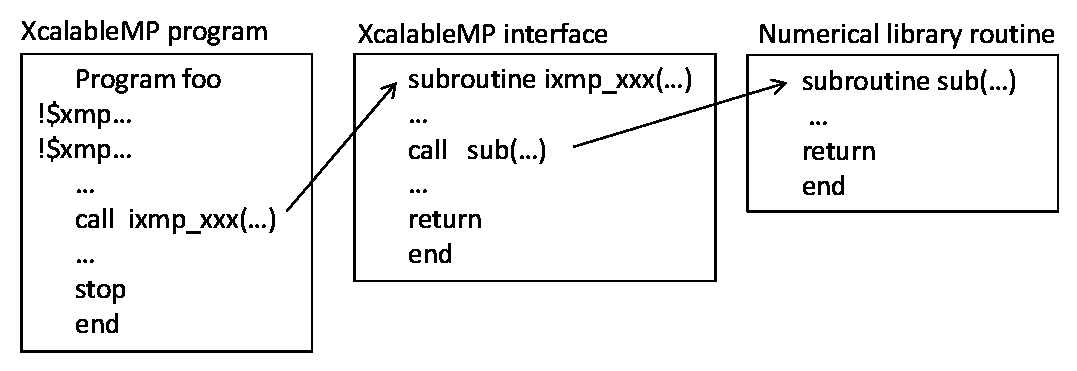
\includegraphics[scale=0.45]{figs/figb.1.eps}
  \caption{Invocation of a Library Routine through an Interface Procedure}
  \label{figb.1}
 \end{myfigure}

 \item When the numerical library routine needs information on an global
       array, the interface extracts it from the descriptor using some
       query routines provided by {\XMP} and passes it to the
       numerical library routine as arguments.
%
 \item The interface does not affect the behavior of numerical library
       routines except for restrictions concerning the {\XMP}
       specification.
\end{itemize}


\section{Query routines}

Specifications of some query routines are shown below.

\subsection{\tt xmp\_node\_index}
\index{xmp\_node\_index@{\tt xmp\_node\_index}}

\subsubsection*{Format}

\begin{tabular}{lll}

\verb![F]!& {\tt subroutine}& {\tt xmp\_node\_index(d, idx)}\\
          & {\tt integer(kind=xmp\_desc\_kind)} & {\tt d}\\
          & {\tt integer} & {\tt idx(dim)}\\

\verb![C]!&  {\tt void}& {\tt xmp\_node\_index(xmp\_desc\_t d, int idx[])}\\

\end{tabular}

\subsubsection*{Synopsis}

The {\tt xmp\_node\_index} routine provides the indices of the
executing node in the target node array.

\subsubsection*{Arguments}

\begin{itemize}
 \item {\tt d} is a descriptor, that is, an object of type {\tt
       integer(kind=xmp\_desc\_kind)}, in {\XMP}, or {\tt xmp\_desc\_t},
       in {\XMPC}, that is associated with the node array.
 \item {\tt idx} is a one-dimensional integer array. {\tt
       dim} is the rank of the node array.
\end{itemize}


\subsection{\tt xmp\_node\_size}
\index{xmp\_node\_size@{\tt xmp\_node\_size}}

\subsubsection*{Format}

\begin{tabular}{lll}

\verb![F]!& {\tt subroutine}& {\tt xmp\_node\_size(d, size)}\\
          & {\tt integer(kind=xmp\_desc\_kind)} & {\tt d}\\
          & {\tt integer} & {\tt size(dim)}\\

\verb![C]!&  {\tt void}& {\tt xmp\_node\_size(xmp\_desc\_t d, int size[])}\\

\end{tabular}

\subsubsection*{Synopsis}

The {\tt xmp\_node\_size} routine provides the size of each dimension of
the target node array.

\subsubsection*{Arguments}

\begin{itemize}
 \item {\tt d} is a descriptor, that is, an object of type {\tt
       integer(kind=xmp\_desc\_kind)}, in {\XMP}, or {\tt xmp\_desc\_t},
       in {\XMPC}, that is associated with the node array.
 \item {\tt size} is a one-dimensional integer array. {\tt
       dim} is the rank of the node array.
\end{itemize}

\subsection{\tt xmp\_gt\_size}
\index{xmp\_gt\_size@{\tt xmp\_gt\_size}}

\subsubsection*{Format}

\begin{tabular}{lll}

\verb![F]!& {\tt subroutine}& {\tt xmp\_gt\_size(d, size)}\\
          & {\tt integer(kind=xmp\_desc\_kind)} & {\tt d}\\
          & {\tt integer} & {\tt size(dim)}\\

\verb![C]!&  {\tt void}& {\tt xmp\_gt\_size(xmp\_desc\_t d, int size[])}\\

\end{tabular}

\subsubsection*{Synopsis}

The {\tt xmp\_gt\_size} routine provides the global size of each
dimension of the target template.

\subsubsection*{Arguments}

\begin{itemize}
 \item {\tt d} is a descriptor, that is, an object of type {\tt
       integer(kind=xmp\_desc\_kind)}, in {\XMP}, or {\tt xmp\_desc\_t},
       in {\XMPC}, that is associated with the target template.
 \item {\tt size} is a one-dimensional integer array. {\tt
       dim} is the rank of the template.
\end{itemize}

\subsection{\tt xmp\_lt\_size}
\index{xmp\_lt\_size@{\tt xmp\_lt\_size}}

\subsubsection*{Format}

\begin{tabular}{lll}

\verb![F]!& {\tt subroutine}& {\tt xmp\_lt\_size(d, size)}\\
          & {\tt integer(kind=xmp\_desc\_kind)} & {\tt d}\\
          & {\tt integer} & {\tt size(dim)}\\

\verb![C]!&  {\tt void}& {\tt xmp\_lt\_size(xmp\_desc\_t d, int size[])}\\

\end{tabular}

\subsubsection*{Synopsis}

The {\tt xmp\_lt\_size} routine provides the local size of each dimension
of the target template.

\subsubsection*{Arguments}

\begin{itemize}
 \item {\tt d} is a descriptor, that is, an object of type {\tt
       integer(kind=xmp\_desc\_kind)}, in {\XMP}, or {\tt xmp\_desc\_t},
       in {\XMPC}, that is associated with the template.
 \item {\tt size} is a one-dimensional integer array. {\tt
       dim} is the rank of the template.
\end{itemize}


\subsection{\tt xmp\_ga\_size}
\index{xmp\_ga\_size@{\tt xmp\_ga\_size}}

\subsubsection*{Format}

\begin{tabular}{lll}

\verb![F]!& {\tt subroutine}& {\tt xmp\_ga\_size(d, size)}\\
          & {\tt integer(kind=xmp\_desc\_kind)} & {\tt d}\\
          & {\tt integer} & {\tt size(dim)}\\

\verb![C]!&  {\tt void}& {\tt xmp\_ga\_size(xmp\_desc\_t d, int size[])}\\

\end{tabular}

\subsubsection*{Synopsis}

The {\tt xmp\_ga\_size} routine provides the global size of each
dimension of the target global array.

\subsubsection*{Arguments}

\begin{itemize}
 \item {\tt d} is a descriptor, that is, an object of type {\tt
       integer(kind=xmp\_desc\_kind)}, in {\XMP}, or {\tt xmp\_desc\_t},
       in {\XMPC}, that is associated with the global array.
 \item {\tt size} is to be set to a one-dimensional integer array. {\tt
       dim} is the rank of the global array.
\end{itemize}

\subsection{\tt xmp\_la\_size}
\index{xmp\_la\_size@{\tt xmp\_la\_size}}

\subsubsection*{Format}

\begin{tabular}{lll}

\verb![F]!& {\tt subroutine}& {\tt xmp\_la\_size(d, size)}\\
          & {\tt integer(kind=xmp\_desc\_kind)} & {\tt d}\\
          & {\tt integer} & {\tt size(dim)}\\

\verb![C]!&  {\tt void}& {\tt xmp\_la\_size(xmp\_desc\_t d, int size[])}\\

\end{tabular}

\subsubsection*{Synopsis}

The {\tt xmp\_la\_size} routine provides the local size of each
dimension of the global array.

\subsubsection*{Arguments}

\begin{itemize}
 \item {\tt d} is a descriptor, that is, an object of type {\tt
       integer(kind=xmp\_desc\_kind)}, in {\XMP}, or {\tt xmp\_desc\_t},
       in {\XMPC}, that is associated with the global array.
 \item {\tt size} is a one-dimensional integer array. {\tt
       dim} is the rank of the global array.
\end{itemize}

\subsection{\tt xmp\_ga\_template\_unitsize}
\index{xmp\_ga\_template\_unitsize@{\tt xmp\_ga\_template\_unitsize}}

\subsubsection*{Format}

\begin{tabular}{lll}

\verb![F]!&  {\tt subroutine}& {\tt xmp\_ga\_template\_unitsize(d, unitsize)}\\
          & {\tt integer(kind=xmp\_desc\_kind)} & {\tt d}\\
          & {\tt integer} & {\tt unitsize(dim)}\\

\verb![C]!&  {\tt void}& {\tt xmp\_ga\_template\_unitsize(xmp\_desc\_t d, int unitsize[])}\\

\end{tabular}

\subsubsection*{Synopsis}

The {\tt xmp\_ga\_template\_unitsize} routine provides the blocking
factor of each dimension of the target template.

\subsubsection*{Arguments}

\begin{itemize}
 \item {\tt d} is a descriptor, that is, an object of type {\tt
       integer(kind=xmp\_desc\_kind)}, in {\XMP}, or {\tt xmp\_desc\_t},
       in {\XMPC}, that is associated with the template.
 \item {\tt unitsize} is a one-dimensional integer array. {\tt dim} is
       the rank of the template.
\end{itemize}


\subsection{\tt xmp\_ga\_first\_idx\_node\_index}
\index{xmp\_ga\_first\_idx\_node\_index@{\tt
xmp\_ga\_first\_idx\_node\_index}}

\subsubsection*{Format}

\begin{tabular}{lll}

\verb![F]!&  {\tt subroutine}& {\tt xmp\_ga\_first\_idx\_node\_index(d, idx)}\\
          & {\tt integer(kind=xmp\_desc\_kind)} & {\tt d}\\
          & {\tt integer} & {\tt idx(dim)}\\

\verb![C]!&  {\tt void}& {\tt xmp\_ga\_first\_idx\_node\_index(xmp\_desc\_t d, int idx[])}\\

\end{tabular}

\subsubsection*{Synopsis}

The {\tt xmp\_ga\_first\_idx\_node\_index} routine provides the indices
of the node onto which the {\it first} element of the global array is
distributed.

\subsubsection*{Arguments}

\begin{itemize}
 \item {\tt d} is a descriptor, that is, an object of type {\tt
       integer(kind=xmp\_desc\_kind)}, in {\XMP}, or {\tt xmp\_desc\_t},
       in {\XMPC}, that is associated with the global array.
 \item {\tt idx} is a one-dimensional integer array. {\tt dim} is the
       rank of node array associated with the global array.
\end{itemize}


\subsection{\tt xmp\_la\_lead\_dim}
\index{xmp\_la\_lead\_dim@{\tt xmp\_la\_lead\_dim}}

\subsubsection*{Format}

\begin{tabular}{lll}

\verb![F]!&  {\tt subroutine}& {\tt xmp\_la\_lead\_dim(d, lead\_dim)}\\
          & {\tt integer(kind=xmp\_desc\_kind)} & {\tt d}\\
          & {\tt integer} & {\tt lead\_dim}\\

\verb![C]!&  {\tt void}& {\tt xmp\_la\_lead\_dim(xmp\_desc\_t d, int lead\_dim)}\\

\end{tabular}

\subsubsection*{Synopsis}

The {\tt xmp\_la\_lead\_dim} routine provides the leading dimension of
each local section of the target global array.

\subsubsection*{Arguments}

\begin{itemize}
 \item {\tt d} is a descriptor, that is, an object of type {\tt
       integer(kind=xmp\_desc\_kind)}, in {\XMP}, or {\tt xmp\_desc\_t},
       in {\XMPC}, that is associated with the global array.
 \item {\tt lead\_dim} is an integer scalar.
\end{itemize}


%\subsection{\tt xmp\_la\_addr}
%
%\subsubsection*{Format}
%
%\begin{tabular}{lll}
%
%\verb![F]!&  {\tt subroutine}& {\tt xmp\_la\_addr(d, addr)}\\
%          & {\tt xmp\_desc\_t} & {\tt d}\\
%          & {\tt integer, allocatable} & {\tt addr}\\
%
%\verb![C]!&  {\tt void}& {\tt xmp\_la\_addr(xmp\_desc\_t d, int* addr)}\\
%
%\end{tabular}
%
%\subsubsection*{Synopsis}
%
%The {\tt xmp\_la\_addr} routine provides the base address of each local
%section of the target global array.
%
%\subsubsection*{Arguments}
%
%\begin{itemize}
% \item {\tt d} is a descriptor, that is, an object of type {\tt
%       xmp\_desc\_t} that is associated with the global array.
% \item {\tt addr} is the base address of the local array.
%\end{itemize}


\section{Example}
\index{Example!library interface}

   This section shows the interface to ScaLAPACK as an example of the
   {\XMP} interface to numerical libraries.
   
   ScaLAPACK is a linear algebra library for distributed-memory.
   Communication processes in the ScaLAPACK routines depends on BLACS
   (Basic Linear Algebraic Communication Subprograms).
   ScaLAPACK library routines invoked from {\XMP} procedures also depend
   on BLACS. %Remarks of the design of the interface are as follows.

%\begin{itemize}
%\item For a ScaLAPACK library routine having a descriptor array as an
%      argument, the interface procedure has the BLACS context handle
%      including the descriptor array as an additional argument.
%\item The {\tt blacs\_exit} routine is unnecessary because an {\XMP}
%      program executes {\tt MPI\_Finalize}.
%\item Only ``column-major'' is effective as the argument ``order'' of a
%      BLACS routine {\tt blacs\_gridinit}.
%\end{itemize}

\begin{description}

 \item[Example 1]
	    This example shows an implementation of the interface for
	    the ScaLAPACK driver routine {\tt pdgesv}.

\begin{XFexample}
      subroutine ixmp_pdgesv(n,nrhs,a,ia,ja,da,ipiv,b,ib,jb,db,ictxt,info)

      use xmp_lib

      integer n,nrhs,ia,ja,ib,jb,ictxt,info
      double precision a,b
      integer(kind=xmp_desc_kind) da,db
      integer size_a(2),unitsize_a(2),rank_a(2),lead_dim_a,desca(9)
      integer size_b(2),unitsize_b(2),rank_b(2),lead_dim_b,descb(9)
      
      call xmp_ga_size(da,size_a)
      call xmp_ga_template_unitsize(da,unitsize_a)
      call xmp_ga_first_idx_nodes_rank(da,rank_a)
      call xmp_la_lead_dim(da,lead_dim_a)
      
      call xmp_ga_size(db,size_b)
      call xmp_ga_template_unitsize(db,unitsize_b)
      call xmp_ga_first_idx_nodes_rank(db,rank_b)
      call xmp_la_lead_dim(db,lead_dim_b)
      
      desca(1)=1
      desca(2)=ictxt
      desca(3)=size_a(1)
      desca(4)=size_a(2)
      desca(5)=unitsize_a(1)
      desca(6)=unitsize_b(2)
      desca(7)=rank_a(1)
      desca(8)=rank_a(2)
      desca(9)=lead_dim_a
      
      descb(1)=1
      descb(2)=ictxt
      descb(3)=size_b(1)
      descb(4)=size_b(2)
      descb(5)=unitsize_b(1)
      descb(6)=unitsize_b(2)
      descb(7)=rank_b(1)
      descb(8)=rank_b(2)
      descb(9)=lead_dim_b
      
      call pdgesv(n,nhrs,a,ia,ja,desca,ipiv,b,ib,jb,descb,info)
      
      return
      end

\end{XFexample}


\item[Example 2]
	   This example shows an {\XMP} procedure using the interface of
	   Example 1.

\Example{nodes}
\Example{template}
\Example{distribute}
\Example{align}
\Example{loop}
\begin{XFexample}
      program xmptdgesv

      use xmp_lib

      double precision a(1000,1000)
      double precision b(1000)
      integer ipiv(2*1000,2)
!$xmp nodes p(2,2)
!$xmp template t(1000,1000)
!$xmp template t1(2*1000,2)
!$xmp distribute t(block,block) onto p
!$xmp distribute t1(block,block) onto p
!$xmp align a(i,j) with t(i,j)
!$xmp align ipiv(i,j) with t1(i,j)
!$xmp align b(i) with t(i,*)
      ...
      integer i,j,ictxt
      integer m=1000,n=1000,nprow=2,npcol=2
      integer icontxt=-1,iwhat=0
      integer nrhs=1,ia=1,ja=1,ib=1,jb=1,info
      character*1 order
      ...
      order="C"
      ...
      call blacs_get(icontxt,iwhat,ictxt)
      call blacs_gridinit(ictxt,order,nprow,npcol)
      ...
!$xmp loop (i,j) on t(i,j)
      do j=1,n
         do i=1,m
            a(i,j) = ...
         end do
      end do
      ...
!$xmp loop on t(i,*)
      do i=1,m
         b(i)= ...
      end do
      ...
      call ixmp_pdgesv(n,nrhs,a,ia,ja,xmp_desc_of(a),ipiv,
     *                b,ib,jb,xmp_desc_of(b),ictxt,info)
      ...
      call blacs_gridexit(ictxt)
      ...
      stop
      end
\end{XFexample}
\end{description}

\cleardoublepage


 \chapter{XcalableMP I/O(Proposal)}

 \section{Categorization of I/O}
 XcalableMP has three kinds of I/O.

  \subsection{Local I/O}

  Local I/O is the way to use I/O statements and I/O service functions in
  base languages, in which I/O statements and functions are used without
  any directives.

  I/O statements (in {\XMP} {\Fort}) and I/O functions (in {\XMP} {\C})
  are executed in local similar to the other execution statements.
  It depends on the system which nodes can handle the I/O statements and
  functions.

  Local I/O can read a file written by the base language and, vice
  versa.

  [F] A name of a global array in the I/O list describes the
  entire area of the array located in each node.

  An array element of a global array can be referred as an I/O item only
  in the node where it is located.

  [F] Any array section of a global array cannot be referred as an
  I/O item.

  \subsection{Master I/O[F]}

  Master I/O is input and output for the file that corresponds to an
  execution node set.
  Master I/O is global execution.

  In master I/O, a global data is input and output as if it is executed
  only by master node, which represents the execution node set, through
  its local copy of the data.

  Master node is chosen among the execution node set arbitrarily by the
  system, and is unique to the execution node set during execution of
  the program.

  Master I/O is provided in the form of directives of {\XMP} {\Fort}.

  A global array as an I/O item is accessed in the sequential order of
  array elements.
  When a local variable is read from a file, the value is copied to all
  nodes of the execution node set.
  When a local variable or an expression is written to a file, only the
  value of the data on master node is written.
  
  Master I/O can read a file written by the base language, and vice
  versa.
  

  \subsection{Global I/O}

  Also global I/O is input and output for the file that corresponds to
  an execution node set.
  Some executions of global I/O are global and the others are local.
  In a large system with many nodes, global I/O can be expected higher
  speed and less memory consumption execution than master I/O.

  [F] It is provided in the form of directives for a part of I/O
  statements, such as OPEN, CLOSE, READ
  and WRITE statements.

  [C] It is provided in the form of service functions and include files.

  Global I/O can handle only unformatted (binary) files. In XcalableMP Fortran,
  implied DO-Loops and some specifiers cannot be used.
  In XcalableMP C, a formatted I/O library, including fprintf() and fscanf(), is not provided.

  Global I/O can read a file written in MPI-IO, and vice versa. 

  [F] File formats are not compatible between XcalableMP Fortran
  and the base language because global I/O does not generate or access
  the file header and footer particular to the base language.

  There are three kinds of Global I/O, as shown in Table
  \ref{tb:global}.
  {\bf Collective} global I/O is global (collective) execution and
  sequential file access.
  It handles global data in the sequential order, similar to master
  I/O.
  {\bf Atomic} global I/O is local execution and sequential file access.
  Execution nodes share file positioning of the global I/O file and
  execute each I/O statement and library call mutually.
  {\bf Direct} global I/O is local execution and direct file access.
  Each execution node has its own file positioning and accesses a shared
  file concurrently.

  \begin{table}[tb]
   \begin{center}
    \caption{Global I/O}
    \label{tb:global}
    \begin{tabular}{|c||l|l|}
     \hline 
     & independent/collective & access method  \\ \hline \hline
     Collectibe I/O & collective & sequential access \\ \hline
     Atomic I/O & independent & sequential access \\ \hline
     Direct I/O & independent & direct access \\ \hline
    \end{tabular}
   \end{center}
  \end{table}
  
  Restriction

  \begin{itemize}
   \item  The name of a global array may not be declared in a namelist
	  group.
	  That is, NAMELIST I/O is not allowed for global arrays.
  \end{itemize}

  Advice for programmers

  Local I/O is useful for debugging focusing on a node since local I/O
  is executed on each node individually.

  Master I/O is a directive extension, in which the execution result
  matches the one of the base language ignoring directive lines.

  Global I/O aims for highly-parallel I/O using thousands of nodes.
  It is limited to binary file.
  It avoids extreme concentration of computational load and memory
  consumption to specific nodes using MPI-IO or other parallel I/O
  techniques.

  \section{File Connection}

  A file is connected to a unit in XcalableMP Fortran and to a file
  handler in XcalableMP C.
  This operation is called {\bf file connection}.
  Local I/O connects a file in each node independently.
  Master I/O and global I/O connect a file to an execution node set
  collectively.
  
  There are two ways of file connections, dynamic connection and
  preconnection.
  Dynamic connection connects a file during execution of the program.
  Preconnection connects a file at the begininng of execution of the
  program and therefore it can execute I/O statements and functions
  without the prior execution of an OPEN statement or a function call to
  open the file.

  \subsection{File connection in local I/O}

  The language processor of the base language connects the file in each
  node.
  File system visible to each node is implementation dependent.

  It is implementation dependent which nodes can access the standard
  input, output and error files.
  It is also implementation dependent how behave the nodes accessing the
  same file at the same time; e.g., data in the standard input file may
  be read only one node and may be replicated all nodes.
  It is implementation dependent how data from the multiple nodes are
  merged into the standard output/error file.
  
  \subsection{File connection in master I/O [F]}

  An OPEN statement specified with a master I/O directive connects the
  master I/O file to the execution node set.
  When a master I/O file is connected by a READ statement or a WRITE
  statement without encountering any OPEN statement, the name and
  attribute of the file depend on the language system of the base
  language.
  Disconnection from a master I/O file is executed by a CLOSE statement
  or termination of the program.

  Dynamic connection must be executed concurrently by all nodes sharing
  the file with the same unit number.
  Two execution node sets may employ the same unit number only if they
  have no common node.

  The standard input, output and error files are preconnected to the
  entire node set.
  Therefore, master I/O executed on the entire node set is always
  allowed without OPEN and CLOSE statements.


  \subsection{File connection in global I/O}

  Dynamic connecton of global I/O is global (collective) execution and
  is valid for the execution node set.
  Global I/O file cannot be preconnected.

  \subsubsection*{[F]}

  An OPEN statement specified with a global I/O directive connects the
  global I/O file to the execution node set.
  Disconnection from a global I/O file is executed by a CLOSE statement
  or termination of the program.

  Dynamic connection must be executed concurrently by all nodes sharing
  the file with the same unit number.
  Two execution node sets may employ the same unit number only if they
  have no common node.

  \subsubsection*{[C]}

  A library function to open a global I/O file connect the file to the
  execution node set.
  Disconnection from a global I/O file is executed by a library function
  to close the file or termination of the program.

  \section{Master I/O}

  \subsection*{Summary}
  A master I/O construct executes data transfer between a file and an
  execution node set via master node of the execution node set.
  For a global array, the virtual sequential order of the array elements
  is visible.

  \subsection*{Syntax}
%  \Syntax{tasks}

  \begin{tabular}{ll}
   \verb![F]! & \verb|!$xmp| {\tt \verb|master_io|} \\
   & \hspace{5mm} {\it io-statement} \\
   & \\
   \verb![F]! & \verb|!$xmp| {\tt \verb|master_io|} begin \\
   & \hspace{5mm}{\it io-statement} \\
   & \hspace{5mm}... \\
   & \verb|!$xmp| {\tt \verb|master_io|} end \\
  \end{tabular}

   where {\it io-statement} is one of:

   \begin{itemize}
    \item OPEN statement
    \item CLOSE statement
    \item READ statement
    \item WRITE statement
    \item PRINT statement
    \item BACKSPACE statement
    \item ENDFILE statement
    \item REWIND statement
    \item INQUIRE statement
   \end{itemize}

   \subsection*{Restriction}
   \begin{itemize}
    \item The following items cannot be specified in the input item list.

	  \begin{itemize}
	   \item Array section of global array
	   \item Substring of global array
	   \item Array element whose subscript contains reference of a
		 global array
	   \item Array section whose subscript contains reference of a
		 global array
	   \item Substring whose subscript contains reference of a
		 global array
	   \item Expressions including the global array reference
	   \item I/O implied DO
	  \end{itemize}

    \item An I/O statement specified with a master I/O directive must be
	  executed on the node set that is connected to the file.
    \item Internal file I/O is not allowed as a master I/O.
   \end{itemize}
	  
  \subsection*{Description}

   An I/O statement specified with a master I/O directive accesses to a
   file whose format is the same as the one of the base language.
   The access, including connection, disconnection, input and output,
   file positioning, and inquiry, is global (collective) and must be
   executed on the same node set as the one where the file was
   connected. 

   Master node, a unique node to a execution node set, is chosen by the
   language system.
   Master I/O works as if all file access is executed only on the master
   node.

   The operations for I/O items are summarized in the following table.

   \begin{table}[h]
    \begin{center}
     \begin{tabular}{|l|p{40mm}|p{80mm}|}
      \hline
      \multicolumn{1}{|c}{ }  & {\bf I/O item} & {\bf operation} \\
      \hline
      input item & name of global array & The data that is read 
	      from the file in the sequential order of array elements is distributed onto 
	      the global array on the node set. The file positioning increases by
	      the size of data. \\
      \cline{2-3}
      & array element of global array &  The data that is read from the file
	      is copied to the element of the global array on the specific node.
	      The file positioning increases by the size of data. \\
      \cline{2-3}
      & local variable & The data that is read from the file is replicated to the
	      local variables on all nodes of the execution node
	      set. The file positioning increases by the size of data. \\
      \cline{2-3}
      & inplied DO-loop & For each input item, repeats the above operation. \\
      \hline
      output item & name of global array & The value of the
	      global array is collected and is written to the
	      file in the sequential order of array elements. The file
	      positioning increases by the size of data. \\
      \cline{2-3}
      & array element of global array &  The value of the element of the
	      global array is written to the
	      file. A file position increases by data length. \\
      \cline{2-3}
      & local variable and expression & The value evaluated on the master node
	      is written to the file. The file positioning increases by
	      the size of data. \\
      \cline{2-3}
      & inplied DO-loop & For each output item, repeat the above operation. \\
      \hline
      \end{tabular}
     \end{center}
%    \caption{aaa}
    \label{tb:aaa}
   \end{table}

   Namelist input and output statements cannot treat global arrays.
   A namelist output statement writes the value on the master node to
   the file.
   In the namelist input, each item of the namelist is read from the
   file to the master node if it is recorded in the file.
   And then all items of the namelist are replicated onto all nodes of
   the execution node set even if any item is not read from the file.

   IOSTAT and SIZE specifiers and specifiers of the INQUIRE statement
   that can return values always return the same value among the
   execution node set.

   When a condition specified with ERR, END or EOR specifier is
   satisfied, all nodes of execution node set are branched together to
   the same statement.

   Advice to the implementer

   It is recommended to provide such a compiler option that local I/O
   statements (specified without directives) is regarded as master I/O
   statements (specified with master\_io directives).

   \clearpage
   
   \section{Global I/O}

   Global I/O executes data transfer between a file and global arrays
   distributed on the execution node set.
   Global I/O is restricted within unformatted (binary) files, but
   higher performance and lower memory consumption can be expected than
   master I/O.
   The file format is compatible with the one in MPI-IO.

   Global I/O consists of three kinds, collective I/O, atomic I/O, and
   direct I/O. 

   \subsection{Global I/O construct [F]}
   \subsubsection*{Syntax}

   \begin{tabular}{ll}
   \verb![F]! & \verb|!$xmp| {\tt \verb|global_io|} [atomic / direct] \\
   & \hspace{5mm} {\it io-statement} \\
   & \\
   \verb![F]! & \verb|!$xmp| {\tt \verb|global_io|} [atomic / direct] begin \\
   & \hspace{5mm}{\it io-statement} \\
   & \hspace{5mm}... \\
   & \verb|!$xmp| {\tt \verb|global_io|} end \\
   \end{tabular}

   The first syntax is just a shorthand of the second syntax.

   \subsubsection*{Restriction}

   I/O statements and specifiers available for {\it io-statement} is
   shown in the following table.
   Definition of each specifier is described in the specification of the base language. 

   Case of global\_io construct without direct clause:
   \begin{table}[h]
   \begin{center}
    \label{tb:globalstatement}
    \begin{tabular}{|c||l|}
      \hline
     I/O statement & available specifiers \\ \hline \hline
     OPEN & UNIT, IOSTAT, FILE, STATUS, POSITION, ACTION \\ \hline
     CLOSE & UNIT, IOSTAT, STATUS \\ \hline
     READ & UNIT, IOSTAT \\ \hline
     WRITE & UNIT, IOSTAT \\ \hline
    \end{tabular}
   \end{center}
   \end{table}

   Case of global\_io construct with direct clause:
   \begin{table}[h]
   \begin{center}
    \label{tb:globalstatement}
    \begin{tabular}{|c||l|}
      \hline
     I/O statement & available specifiers \\ \hline \hline
     OPEN & UNIT, IOSTAT, FILE, STATUS, RECL, ACTION \\ \hline
     CLOSE & UNIT, IOSTAT, STATUS \\ \hline
     READ & UNIT, REC, IOSTAT \\ \hline
     WRITE & UNIT, REC, IOSTAT \\ \hline
    \end{tabular}
   \end{center}
   \end{table}

   Only the name of a variable (including global variable) can be specified 
   as the input item of READ statement specified with global\_io directive,
   but array element, array section,
   structure component, substring, and implied-DO loop are not allowed as input items.

   Only the name of a global array and an
   expression excluding global array reference can be specified as the output item
   of WRITE statement specified with global\_io directive, 
   but an expression including global array
   reference and implied-DO loop are not allowed as input items.


   \subsubsection*{Description}

   Global I/O construct connects, disconnects, inputs and outputs the global I/O file,
   which is compatible with MPI-IO.

   The standard input, output and error files cannot be a Global I/O file.
   A Global I/O file cannot preconnect to any unit or any file handler,
   and must explicitly be connected by the OPEN statement specified with
   global\_io directive.

   The OPEN statement specified with global\_io directive is global
   (collective) execution, and the file is shared in the execution node
   set.
   A file that is already open by the other OPEN statement with
   global\_io directive cannot be reopen by an OPEN statement with or
   without global\_io directive.

   A global I/O file must be disconnected explicitly by a CLOSE
   statement specified with global\_io directive, else the result of I/O
   is not guaranteed.
   The CLOSE statement specified with global\_io directive is a global
   (collective) execution and must be executed by the same execution
   node set as the one where the OPEN statement is executed.

   Available values of the specifiers in I/O statements are shown in the
   following table.
   Definitions of the specifiers are described in the specification of
   the base language.

   \begin{itemize}
    \item OPEN statement
   
   \begin{table}[h]
    \begin{center}
     \label{tb:globalopen}
     \begin{tabular}{|c||p{90mm}|l|}
       \hline
      specifiers & value & default \\ \hline \hline
      UNIT & external file unit (scalar constant expression)
	  & not omissible. \\ \hline
      FILE & file name (scalar CHARACTER expression)
	  & not omittable. \\ \hline
      STATUS & 'OLD', 'NEW', 'REPLACE' or 'UNKNOWN' & 'UNKNOWN' \\ \hline
      POSITION\footnote{available only if the directive has no directive
      clause} & 'ASIS', 'REWIND' or 'APPEND' & 'ASIS' \\ \hline
      ACTION & 'READ', 'WRITE' or 'READWRITE' & 'READWRITE' \\ \hline
      RECL\footnote{available only if the directive has a directive clause} & the value of the record length (scalar constant expression)
	  & not omittable. \\ \hline
     \end{tabular}
    \end{center}
   \end{table}

    \item CLOSE statement
	  
   \begin{table}[h]
    \begin{center}
     \label{tb:globalopen}
     \begin{tabular}{|c||p{90mm}|l|}
        \hline
      specifiers & value & default \\ \hline \hline
      UNIT & external file unit (scalar constant expression)
	  & omittable. \\ \hline
      STATUS & 'KEEP' or 'DELETE'
	  & 'KEEP' \\ \hline
     \end{tabular}
    \end{center}
   \end{table}

    \item READ/WRITE statement
	  
   \begin{table}[h]
    \begin{center}
     \label{tb:globalopen}
     \begin{tabular}{|c||p{90mm}|l|}
       \hline
      specifiers & value & default \\ \hline \hline
      UNIT & external file unit (scalar constant expression)
	  & not omittable. \\ \hline
      REC\footnote{available only if the directive has a directive clause} & the value of the record length (scalar constant expression)
	  & not omittable. \\ \hline
     \end{tabular}
    \end{center}
   \end{table}

    \item When a scalar default INTEGER variable is set to IOSTAT, an
	  error code is set to the specifiers.
	 
   \end{itemize}

   OPEN, CLOSE, READ and WRITE statements specified with global\_io directives
   without atomic and direct clauses are called respectively collective OPEN, collective
   CLOSE, collective READ, and collective WRITE statements respectively.
   These all statements are called collective I/O statements.

   OPEN, CLOSE, READ and WRITE statements specified with global\_io directives
   with atomic clauses are called atomic OPEN, atomic CLOSE, atomic READ, and
   atomic WRITE statements respectively.
   These all statements are called atomic I/O statements.

   OPEN, CLOSE, READ and WRITE statements specified with global\_io directives
   with direct clause are called direct OPEN, direct CLOSE, direct READ, and
   direct WRITE statements respectively.
   These all statements are called direct I/O statements.

   The file connected by collective, atomic or direct OPEN statement can
   be read/be written only by the same type of READ/WRITE statement.
   The file can be disconnected by the same type of CLOSE statement.
   Different types of global I/O cannot be executed together for the same file or the
   same unit.
   For example, atomic I/O statements cannot be executed for the unit
   connected by a collective OPEN statement.

   \clearpage
   
   \subsubsection{collective I/O statement}

   Collective I/O statements read/write for a file shared between nodes.
   I/O data remains the image of global array.

   Collective I/O statements are matched across all nodes.
   In collective I/O, I/O operations, such as connection, disconnection,
   read and write, for a file must be executed in the same nodes. 
   
   The operations for I/O items are summarized in the following table.

   \begin{table}[h]
    \begin{center}
     \begin{tabular}{|l|r|p{80mm}|}
      \hline
      \multicolumn{1}{|c}{ }  & {\bf I/O item} & {\bf operation} \\ \hline
      input item & name of distributed array & The value is read along
	      the file view set in a template. The value is set to array
	      elements in each node.
	      File position seeks by data size.\\
      \cline{2-3}
      & duplicate variable &  The value set from a file is set in a
	      duplicate array in all nodes. File position seeks by
	      data length. \\ \hline
      output item & name of distributed array & The value is written
	      along the file view set in a template. The value is
	      written for a file.
	      File position seeks by data size.\\
      \cline{2-3}
      & duplicate variable, expression & The value in any one node is
	      written to the file.  File position seeks by data
	      length. \\ \hline
      \end{tabular}
     \end{center}
%    \caption{aaa}
    \label{tb:aaa}
   \end{table}

   \subsubsection{atomic I/O statement}

   Atomic I/O statements exclusively read/write for a file shared
   between nodes in no particular order.
   As nondeterministic parallel execution, if the program is the same,
   the results can differ.

   Atomic OPEN and CLOSE statements are executed collectively. Atomic
   READ and WRITE statements are executed locally.
   The file connected by atomic OPEN statements is disconnected by using
   atomic CLOSE statements in all execution nodes.
   Atomic READ and WRITE statements can be executed from any node in a
   set of execution nodes.

   Atomic READ and WRITE statements are exclusively excuted.
   A unit of atomic I/O statements is a READ statement or a WRITE
   statement.

   At first, the file position is determined by the POSITION specifier in
   atomic I/O statement.
   After that, file position seeks by the length of the input/output
   variables.


   \subsubsection{direct I/O statement}

   Direct I/O statements read/write for a file shared between nodes.
   File position is specified on each node.

   Direct OPEN and CLOSE statements are executed collectively. Direct
   READ and WRITE statements are executed locally.
   The file connected by direct OPEN statements is disconnected by using
   atomic CLOSE statements in all execution nodes.
   Direct READ and WRITE statements can be executed from any node in a
   set of execution nodes.
   
   Direct READ and WRITE statements read/write to file position
   specified by a REC specifier.
   Direct READ and WRITE statements are executed independently.
   File position is the value multiplied by the value specified in a RECL
   specifiers and the value specified in a REC specifier.


   \subsection{Global I/O library [C]}

   In C, some of data types is defined in an include file.
   A set of library functions with the arguments of the data type is
   provided.
   Built-in function gotten these type from the name of a distributed
   array is provided.
   The following types are provided.

   \begin{itemize}
    \item xmp\_file\_t : file handle
    \item xmp\_array\_t : distributed data for a distributed
	  array
    \item xmp\_rang\_t : expression of array section
   \end{itemize}

   The following library functions are provided.
   Collective function names end with \_all.

   \begin{itemize}
    \item global I/O file operation
    \begin{itemize}
     \item xmp\_fopen\_all
     \item xmp\_fclose\_all
     \item xmp\_fseek
     \item xmp\_fseek\_shared\_all
     \item xmp\_ftell
     \item xmp\_ftell\_shared
     \item xmp\_file\_sync\_all
    \end{itemize}
    \item collective I/O
    \begin{itemize}
     \item xmp\_file\_set\_view\_all
     \item xmp\_file\_clear\_view\_all
     \item xmp\_fread\_all
     \item xmp\_fwrite\_all
     \item xmp\_fread\_darray\_all
     \item xmp\_fwrite\_darray\_all
    \end{itemize}
    \item atomic I/O
    \begin{itemize}
     \item xmp\_fread\_shared
     \item xmp\_fwrite\_shared
    \end{itemize}
    \item direct I/O
    \begin{itemize}
     \item xmp\_fread
     \item xmp\_fwrite
    \end{itemize}
   \end{itemize}

   \clearpage
   
   \subsubsection{Data type}

   The following data types are defined in include file ``xmp\_io.h''.
   \begin{description}
    \item[xmp\_file\_t] The valiable of xmp\_file\_t type is a file
	       handle.
	       The file handle is generated when a file is opened.
	       There are shared file pointer and intrinsic file pointer
	       to identify file position.

	       Shared file pointer share with shared nodes.
	       The file pointer is seeked by atomic I/O.
	       Identify file pointer is seeked by collective I/O and
	       direct I/O.
	       
	       These file pointers are managed by the member of
	       xmp\_file\_t type structures.
	       These file pointers are controled and referenced through
	       the library function.
	       
    \item[xmp\_array\_t] The valiable of xmp\_array\_t is distributed data
	       for a distributed array.
	       Distribution, alignment and node array shape, etc are the
	       member of xmp\_array\_t.

	       Distributed data of Distributed array ``A'' is gotten by
	       the following built-in function.
	       
	       xmp\_array\_t xmp\_array\_of(A);
	       
    \item[xmp\_range\_t] The valiable of xmp\_range\_t is an expression
	       of array section.
	       Lower bound, upper bound and stride are included in the
	       member of an array.
   \end{description}

   \subsubsection{Global I/O file operation}

   [OPEN]
   
   The function opens a global I/O file.
   \begin{table}[h]
    \begin{center}
      \begin{tabular}{|l|r|p{90mm}|}
      \hline
      {\bf function name}  & \multicolumn{2}{c|}{\bf xmp\_file\_t
      $*$xmp\_fopne\_all()}  \\ \hline
      argument & const char $*$fname & file name \\ \cline{2-3}
      & const char $*$amode & equialent to fopen of POSIX. combination
	      of ``rwa+'' \\ \hline
      return value & xmp\_file\_t$*$ & file structure. NULL is returned
	      when a program abend. \\ \hline
      \end{tabular}
     \end{center}
%    \caption{aaa}
    \label{tb:aaa}
   \end{table}

   File view is initialized. The value of shared file pointer and intrinsic file
   pointer depend on the value of amode.

   \begin{table}
     \begin{center}
    \label{tb:xxx}
    \begin{tabular}{|c|p{120mm}|}
      \hline
     amode & intended purpose \\ \hline \hline
     r &  Open for reading only. File pointer points the beginning of
	 the file.\\ \hline
     r+ & Open an existing file for update (reading and writing). File
	 pointer points the beginning of the file. \\ \hline
     w &  Create for writing. If a file by that name already exists, it
	 will be overwritten. File pointer points the begininng of th file. \\ \hline
     w+ & Create a new file for update (reading and writing). If a file
	 by that name already exists, it will be overwritten. File
	 pointer points the beginning of the file. \\ \hline
     a & Append; open for writing at end-of-file or create for writing
	 if the file does not eist. File pointer points the end of the file. \\ \hline
     a+ & Open for append; open (or create if the file does not exist)
	 for update at the end of the file. File pointer points the
	 beginning of the file. \\ \hline
    \end{tabular}
   \end{center}
   \end{table}


   \clearpage
   [CLOSE]

   The function closes a global I/O file.

   \begin{table}[h]
    \begin{center}
     \begin{tabular}{|l|l|p{80mm}|}
      \hline
      {\bf function name}  & \multicolumn{2}{c|}{\bf xmp\_file\_t
      $*$xmp\_fclose\_all(fh)} \\ \hline \hline
      argument & xmp\_file\_t $*$fh & file structure \\ \hline
      return value & int & 0: normal termination \\
      &  & 1: abnormal termination. fh is NULL. \\
      &  & 2: abnormal termination. error in MPI\_File\_close. \\ \hline
      \end{tabular}
     \end{center}
%    \caption{aaa}
    \label{tb:close}
   \end{table}

   [intrinsic file pointer setting]

   Change the setting of intrinsic file pointer.
   \begin{table}[h]
    \begin{center}
     \begin{tabular}{|l|r|p{70mm}|}
      \hline
      {\bf function name}  & \multicolumn{2}{c|}{\bf int xmp\_fseek(fh,
      offset, whence)}  \\ \hline \hline
      argument & xmp\_file\_t $*$fh & file structure \\ \cline{2-3}
      & long long offset & displacement of current file view from
	      position of whence \\ \cline{2-3}
      & int whence & choose file position \\
      &  & SEEK\_SET: the beginning of the file \\ 
      &  & SEEK\_CUR: current position \\ 
      &  & SEEK\_END: the end of the file \\ \hline
      return value & int & 0: normal termination \\
      &  & an integer othe than 0: abnormal termination \\ \hline
      \end{tabular}
     \end{center}
%    \caption{aaa}
    \label{tb:aaa}
   \end{table}

   \clearpage

   [shared file pointer setting]

   Change the setting of shared file pointer.
   \begin{table}[h]
    \begin{center}
     \begin{tabular}{|l|r|p{80mm}|}
      \hline
      {\bf function name}  & \multicolumn{2}{c|}{\bf int xmp\_fseek\_shared(fh,
      offset, whence)}  \\ \hline \hline
      argument & xmp\_file\_t $*$fh & file structure \\ \cline{2-3}
      & long long offset & displacement of current file view from
	      position of whence \\ \cline{2-3}
      & int whence & choose file position \\
      &  & SEEK\_SET: the beginning of the file \\ 
      &  & SEEK\_CUR: current position \\ 
      &  & SEEK\_END: the end of the file \\ \hline
      return value & int & 0: normal termination \\
      &  & an integer othe than 0: abnormal termination \\ \hline
      \end{tabular}
     \end{center}
%    \caption{aaa}
    \label{tb:aaa}
   \end{table}


   [referece to position of intrinsic file pointer]

   Refer to position of intrinsic file pointer.
   \begin{table}[h]
    \begin{center}
     \begin{tabular}{|l|r|p{80mm}|}
      \hline
      {\bf function name}  & \multicolumn{2}{c|}{\bf long long
      xmp\_ftell(fh)} \\ \hline \hline
      argument & xmp\_file\_t $*$fh & file structure \\ \hline
      return value & long long & Upon successful completion, the
	      function shall open the file and return a non-negative
	      integer representing the lowest numbered unused file
	      descriptor. Otherwise, negative number shall be
	      returned. \\ \hline
      \end{tabular}
     \end{center}
%    \caption{aaa}
    \label{tb:aaa}
   \end{table}
   

   
   [referece for position of shared file pointer]

   Refer to position of shared file pointer.
   \begin{table}[h]
    \begin{center}
     \begin{tabular}{|l|r|p{80mm}|}
      \hline
      {\bf function name}  & \multicolumn{2}{c|}{\bf long long
      xmp\_ftell\_shared(fh)} \\ \hline \hline
      argument & xmp\_file\_t $*$fh & file structure \\ \hline
      return value & long long & Upon successful completion, the
	      function shall open the file and return a non-negative
	      integer representing the lowest numbered unused file
	      descriptor. Otherwise, negative number shall be
	      returned. \\ \hline
      \end{tabular}
     \end{center}
%    \caption{aaa}
    \label{tb:aaa}
   \end{table}
   
   

   [file synchronization]

   File synchronizing.
   Completion of writing for a file from shared nodes is guaranteed.

   \begin{table}[h]
    \begin{center}
     \begin{tabular}{|l|r|p{80mm}|}
      \hline
      {\bf function name}  & \multicolumn{2}{c|}{\bf int
      xmp\_file\_sync\_all(fh)} \\ \hline \hline
      argument & xmp\_file\_t $*$fh & file structure \\ \hline
      return value & int & 0: normal termination \\
      &  & an integer othe than 0: abnormal termination \\ \hline
      \end{tabular}
     \end{center}
%    \caption{aaa}
    \label{tb:aaa}
   \end{table}

   \clearpage

   \subsubsection{collective I/O}

   Collective I/O is collectively executed.
   Collective I/O read/write from position of intrinsic file pointer.
   Assume that file view is previously set, where file view mechanism
   describes relationship between how nodes will access their data
   and how data laid out on disk.
   A detailed the definition of file view mechanism can be found in MPI
   2.0 specificaation.

   [file view setting]

   The function sets file view.

   \begin{table}[h]
    \begin{center}
     \begin{tabular}{|l|r|p{70mm}|}
      \hline
      {\bf function name}  & \multicolumn{2}{c|}{\bf int xmp\_file\_set\_view\_all(fh,
      disp, ap, rp)} \\ \hline \hline
      argument & xmp\_file\_t $*$fh & file structure \\ \cline{2-3}
      & long long disp & displacement from the beginning of the file. \\ \cline{2-3}
      & xmp\_array\_t ap & data of distributed array \\ \cline{2-3}
      & xmp\_range\_t $*$rp & data of accessible range \\ \hline
      return value & int & 0: normal termination \\
      &  & an integer othe than 0: abnormal termination \\ \hline
      \end{tabular}
     \end{center}
%    \caption{aaa}
    \label{tb:aaa}
   \end{table}

   
   [file view initialization]

   The function clears file view.
   Position of shared file pointer and intrinsic file pointer is set to
   disp.
   Element data type and file type is set to MPI\_BYTE.
   
   \begin{table}[h]
    \begin{center}
     \begin{tabular}{|l|r|p{80mm}|}
      \hline
      {\bf function name}  & \multicolumn{2}{c|}{\bf int xmp\_file\_clear\_view\_all(fh,
      disp)} \\ \hline \hline
      argument & xmp\_file\_t $*$fh & file structure \\ \cline{2-3}
      & long long disp & displacement from the beginning of the file. \\ \hline
      return value & int & 0: normal termination \\
      &  & an integer othe than 0: abnormal termination \\ \hline
      \end{tabular}
     \end{center}
%    \caption{aaa}
    \label{tb:aaa}
   \end{table}


   [collective READ for duplicate variable]

   The function collectively reads data from position of shared file
   pointer.

   \begin{table}[h]
    \begin{center}
     \begin{tabular}{|l|r|p{80mm}|}
      \hline
      {\bf function name}  & \multicolumn{2}{c|}{\bf Size\_t
      xmp\_fread\_all(fh, buffer, size, count)}  \\ \hline \hline
      argument & xmp\_file\_t $*$fh & file structure \\ \cline{2-3}
      & void $*$buffer & beginning address of loading valiables \\ \cline{2-3}
      & size\_t size & the size of a loading element of data \\ \cline{2-3}
      & size\_t count & the number of loading data element \\ \hline
      return value & int & Upon successful completion, return the size
	      of loading data. Otherwise, negative number shall be
	      returned. \\ \hline
      \end{tabular}
     \end{center}
%    \caption{aaa}
    \label{tb:aaa}
   \end{table}


   [collective WRITE for duplicate variable]

   The function collectively writes data from position of shared file
   pointer.

   \begin{table}[h]
    \begin{center}
     \begin{tabular}{|l|r|p{80mm}|}
      \hline
      {\bf function name}  & \multicolumn{2}{c|}{\bf size\_t
      xmp\_fwrite\_all(fh, buffer, size, count)}  \\ \hline \hline
      argument & xmp\_file\_t $*$fh & file structure \\ \cline{2-3}
      & void $*$buffer & beginning address of storing valiables \\ \cline{2-3}
      & size\_t size & the size of a storing element of data \\ \cline{2-3}
      & size\_t count & the number of storing data element \\ \hline
      return value & int & Upon successful completion, return the size
	      of storing data. Otherwise, negative number shall be
	      returned. \\ \hline
      \end{tabular}
     \end{center}
%    \caption{aaa}
    \label{tb:aaa}
   \end{table}

   \clearpage
   [collective READ for distributed array]

   The function collectively reads data to distributed array from
   position of shared file pointer.

   \begin{table}[h]
    \begin{center}
     \begin{tabular}{|l|r|p{80mm}|}
      \hline
      {\bf function name}  & \multicolumn{2}{c|}{\bf size\_t
      xmp\_fread\_darray\_all(fh, ap, rp)} \\ \hline
      argument & xmp\_file\_t $*$fh & file structure \\ \cline{2-3}
      & xmp\_array\_t ap & data of distributed array \\ \cline{2-3}
      & xmp\_range\_t $*$rp & data of accessible range \\ \hline
      return value & int & Upon successful completion, return the size
	      of loading data. Otherwise, negative number shall be
	      returned. \\ \hline
      \end{tabular}
     \end{center}
%    \caption{aaa}
    \label{tb:aaa}
   \end{table}

   The function reads data in the range $rp$ for distributed array $ap$.

   [collective WRITE for distributed array]

   The function collectively writes data to distributed array from
   position of shared file pointer.

   \begin{table}[h]
    \begin{center}
     \begin{tabular}{|l|r|p{80mm}|}
      \hline
      {\bf function name}  & \multicolumn{2}{c|}{\bf size\_t
      xmp\_fwrite\_darray\_all(fh, ap, rp)} \\ \hline
      argument & xmp\_file\_t $*$fh & file structure \\ \cline{2-3}
      & xmp\_array\_t ap & data of distributed array \\ \cline{2-3}
      & xmp\_range\_t $*$rp & data of accessible range \\ \hline
      return value & int & Upon successful completion, return the size
	      of loading data. Otherwise, negative number shall be
	      returned. \\ \hline
      \end{tabular}
     \end{center}
%    \caption{aaa}
    \label{tb:aaa}
   \end{table}

   The function writes data in the range $rp$ for distributed array $ap$.

   \clearpage

   \subsubsection{atomic I/O}

   Atomic I/O is locally executed. But the I/O exclusively read/write
   from position fo shared file pointer. Before atomic I/O is executed,
   file view must be cleared.
   
   [Rationale]

   In MPI, when all proceses use shared file pointer, these processes
   must specify the same file view. But xmp\_file\_set\_view\_all
   function set different file view for each node.
   Thus, before atomic I/O is executed, file view must be cleared.

   [atomic read]

   The function exclusively reads data form position of shared file
   pointer.

   \begin{table}[h]
    \begin{center}
     \begin{tabular}{|l|r|p{80mm}|}
      \hline
      {\bf function name}  & \multicolumn{2}{c|}{\bf size\_t
      xmp\_fread\_shared(fh, buffer, size, count)}  \\ \hline \hline
      argument & xmp\_file\_t $*$fh & file structure \\ \cline{2-3}
      & void $*$buffer & beginning address of loading valiables \\ \cline{2-3}
      & size\_t size & the size of a loading element of data \\ \cline{2-3}
      & size\_t count & the number of loading data element \\ \hline
      return value & int & Upon successful completion, return the size
	      of loading data. Otherwise, negative number shall be
	      returned. \\ \hline
      \end{tabular}
     \end{center}
%    \caption{aaa}
    \label{tb:aaa}
   \end{table}


   [atomic read]

   The function exclusively writes data to distributed array from
   position of shared file pointer.

   \begin{table}[h]
    \begin{center}
     \begin{tabular}{|l|r|p{80mm}|}
      \hline
      {\bf function name}  & \multicolumn{2}{c|}{\bf size\_t
      xmp\_write\_shared(fh, ap, rp)} \\ \hline \hline
      argument & xmp\_file\_t $*$fh & file structure \\ \cline{2-3}
      & xmp\_array\_t ap & data of distributed array \\ \cline{2-3}
      & xmp\_range\_t $*$rp & data of accessible range \\ \hline
      return value & int & Upon successful completion, return the size
	      of storing data. Otherwise, negative number shall be
	      returned. \\ \hline
      \end{tabular}
     \end{center}
%    \caption{aaa}
    \label{tb:aaa}
   \end{table}


   \subsubsection{direct I/O}

   Direct I/O is locally exectuted. The I/O exclusively read/write data
   from position of intrinsic file pointer in each node.
   The setting file view is enable.

   [direct read]

   The function reads data from position of instrinsic file
   pointer.
   The function is locally executed.

   \begin{table}[h]
    \begin{center}
     \begin{tabular}{|l|r|p{80mm}|}
      \hline
      {\bf function name}  & \multicolumn{2}{c|}{\bf size\_t
      xmp\_fread(fh, buffer, size, count)} \\ \hline \hline
      argument & xmp\_file\_t $*$fh & file structure \\ \cline{2-3}
      & void $*$buffer & beginning address of loading valiables \\ \cline{2-3}
      & size\_t size & the size of a loading element of data \\ \cline{2-3}
      & size\_t count & the number of loading data element \\ \hline
      return value & int & Upon successful completion, return the size
	      of loading data. Otherwise, negative number shall be
	      returned. \\ \hline
      \end{tabular}
     \end{center}
%    \caption{aaa}
    \label{tb:aaa}
   \end{table}

   [direct write]

   The function write data from position of instrinsic file
   pointer.
   The function is locally executed.

   \begin{table}[h]
    \begin{center}
     \begin{tabular}{|l|r|p{80mm}|}
      \hline
      {\bf function name}  & \multicolumn{2}{c|}{\bf size\_t
      xmp\_fwrite(fh, buffer, size, count)} \\ \hline \hline
      argument & xmp\_file\_t $*$fh & file structure \\ \cline{2-3}
      & void $*$buffer & beginning address of storing valiables \\ \cline{2-3}
      & size\_t size & the size of a storing element of data \\ \cline{2-3}
      & size\_t count & the number of storing data element \\ \hline
      return value & int & Upon successful completion, return the size
	      of storing data. Otherwise, negative number shall be
	      returned. \\ \hline
      \end{tabular}
     \end{center}
%    \caption{aaa}
    \label{tb:aaa}
   \end{table}

   

\cleardoublepage

\chapter{Memory Consistency Model}

\newcommand{\Coloneqq}{\mathrel{\colon\!=}}
\newcommand{\xsync}{\texttt{xmp\_syn}}
\newcommand{\xasync}[1]{\texttt{xmp\_asyn}(#1)}
\newcommand{\waitasync}[1]{\texttt{wait\_async}(#1)}
\newcommand{\fstmt}{\texttt{f\_stmt}}
\newcommand{\F}[2]{\texttt{Fetch}^{#1} \: {#2}}
\newcommand{\E}[2]{\texttt{Execute}^{#1} \: {#2}}
\newcommand{\R}[2]{\texttt{Reflect}^{#1} \: {#2}}

%loop construct is synchronous.  But practically OK?

%array construct is synchronous.  But semantically OK?

This chapter explains a memory consistency model that XcalableMP adopts.

Memory consistency models specify rules about multiple data accesses
to memories.  Since XcalableMP is an extension of the base languages,
its memory consistency model is also defined to be their extension,
that is, XcalableMP follows all the rules that base languages adopt.

In addition, XcalableMP introduces some rules about \emph{global
  view}.  In global view, \emph{global communication constructs} are
used to access distributed data.  Furthermore, distributed data can be
accessed through designating data in local view.  Conversely,
non-distributed data can be accessed through designating distributed
data by using global communication constructs in global view.  These
are not considered under the memory consistency models of the base
language since global view is a new notion which is introduced by
XcalableMP.

Please recall that global communication constructs are collective as
described in Section~\ref{sec:glossary}.

\section{Execution Traces}

This section explains execution traces that Xcalable memory
consistency model admits.

First, instructions are defined as
\[
i \Coloneqq \xsync \mid \xasync{\textit{async-id}} \mid \waitasync{\textit{async-id}} \mid \fstmt
\]
where $\xsync$ denotes a global communication construct with no
\texttt{async} clause, $\xasync{\textit{async-id}}$ denotes a global
communication construct with the clause
$\texttt{async}(\textit{async-id})$,
%$\waitasync{\textit{async-id}}$ denotes a
%\texttt{wait\_async}(\textit{async-id}),
and $\fstmt$ is a statement.

Next, operations are defined as
\[
o \Coloneqq \F{j}{i} \mid \E{j}{i} \mid \R{j}{i}
\]
where $j$ is a positive integer.

Operation $\F{j}{i}$ denotes that instruction $i$ is fetched at $j$
times.  The integer $j$ is incremented whenever you break or exit
loops.  The instructions that are called at multiple times in loops
are indentified by $j$s.  Operation $\E{j}{i}$ denotes that
instruction $i$ is executed.  Operation $\R{j}{i}$ denotes that effect
of instruction $i$ is reflected to physical memories.

Finally, the memory consistency model defines constraints written by a
partial order $\leq$ on operations as described below.  Execution
traces are defined as sequences of operations that follow the order.
In the following, $o_1 < o_2$ denotes $o_1 \leq o_2$ and $o_1
\not\equiv o_2$, and $o_1 < o_2 < o_3$ denotes $o_1 < o_2$ and $o_2 <
o_3$.

{
\renewcommand{\theequation}{\roman{equation}}
\begin{figure}[htbp]
\begin{align}
& \F{j_1}{i_1} < \F{j_2}{i_2} \mbox{ implies } \E{j_1}{i_1} < \E{j_2}{i_2} \label{constraints:fetchorder}\\
& \E{j_1}{\xsync} < \E{j_2}{i_2} \mbox{ implies } \R{j_1}{\xsync} < \E{j_2}{i_2} \label{constraints:synchronous}\\
& \E{j_1}{\xasync{\textit{async-id}}} < \E{j_3}{\waitasync{\textit{async-id}}} < \E{j_2}{i_2} \mbox{ implies} \nonumber\\
& \R{j_1}{\xasync{\textit{async-id}}} < \E{j_2}{i_2} \label{constraints:asynchronous}
\end{align}
\caption{Constraints that XcalableMP memory consistency model obligates}\label{fig:constraints}
\end{figure}
}

\subsection{Common Constraints}

This subsection explains some constraints that are common between
synchronous and asynchronous communications.

In XcalableMP memory consistency model, instructions are executed in
the order in which they are fetched.  Formally, this is represented by
\ref{constraints:fetchorder} in Figure~\ref{fig:constraints}.

\subsection{Constraints for Synchronous Communications}

The constructs \texttt{reflect}, \texttt{gmove} (and its following
assignment statement), \texttt{reduction}, and \texttt{bcast} are
synchronous if \texttt{async} is not specified.  It means that
executions of these constructs guarantee completions of data
synchronizations, that is, global communication constructs read data
that are written by statements that are previously executed, and their
following statements and global communication constructs read data
written by global communication constructs.  Formally, this is
represented by \ref{constraints:synchronous} in
Figure~\ref{fig:constraints}

For example, in the following code, the assignment statement
\texttt{g(:)=h(:)} is guaranteed to be completed before the second
\texttt{gmove} construct is executed.  Therefore, the value of
\texttt{g(i)} must be \texttt{i} when the assignment statement
\texttt{x(:)=g(:)} is executed.

Finally, the value of \texttt{x(i)} on \texttt{p(1)} must be
\texttt{i}.

\begin{center}
\begin{XFexample}
!$xmp nodes p(2)
!$xmp template t(10)
!$xmp distribute (block) onto p :: t
      integer :: g(10), h(10)
!$xmp align (i) with t(i) :: g, h
      integer x(5)

!$xmp loop on t(i)
      do i=1,10
      h(i)=i
      end do

!$xmp gmove
      g(:)=h(:)
!$xmp gmove
      x(:)=g(:)
\end{XFexample}
\end{center}

\subsection{Constraints for Asynchronous Communications}

The constructs \texttt{reflect}, \texttt{gmove} (and its following
assignment statement), \texttt{reduction}, and \texttt{bcast} are
asynchronous if \texttt{async}s are specified.  Completions of data
read and written by these global communication constructs are not
guaranteed until \texttt{wait\_async}s are executed.
Formally, this is represented by
\ref{constraints:asynchronous} in Figure~\ref{fig:constraints}.

For example, in the following code, the assignment statement
\texttt{g(:)=h(:)} may not be completed before the second
\texttt{gmove} construct is executed since the first \texttt{gmove}
construct has \texttt{async} clause.  Therefore, the value of
\texttt{g(i)} is not guaranteed to be \texttt{i}.

Finally, the value of \texttt{x(i)} on \texttt{p(1)}
is guaranteed to be \texttt{i}.
\begin{center}
\begin{XFexample}
!$xmp nodes p(2)
!$xmp template t(10)
!$xmp distribute (block) onto p :: t
      integer :: g(10), h(10)
!$xmp align (i) with t(i) :: g, h
      integer x(5)

!$xmp loop on t(i)
      do i=1,10
      h(i)=i
      end do

!$xmp gmove async(1)
      g(:)=h(:)
!$xmp gmove
      x(:)=g(:)
!$xmp wait_async(1)
\end{XFexample}
\end{center}

The \texttt{wait\_async(\textit{async-id})} guarantees a completion of
a global communication construct that has \textit{async-id}.
Therefore, the value of \texttt{x(i)} is not guaranteed to be
\texttt{i} in the following program:
\begin{center}
\begin{XFexample}
!$xmp nodes p(2)
!$xmp template t(10)
!$xmp distribute (block) onto p :: t
      integer :: g(10), h(10)
!$xmp align (i) with t(i) :: g, h
      integer x(5)

!$xmp loop on t(i)
      do i=1,10
      h(i)=i
      end do

!$xmp gmove async(1)
      g(:)=h(:)
!$xmp wait_async(1)
!$xmp gmove
      x(:)=g(:)
\end{XFexample}
\end{center}

Assignment statements in local view and \texttt{gmove} constructs in
global view may race.  The value of \texttt{x(5)} is not guaranteed to
be \texttt{6}, and may be \texttt{5} in the following program:
\begin{center}
\begin{XFexample}
!$xmp nodes p(2)
!$xmp template t(10)
!$xmp distribute (block) onto p :: t
      integer :: g(10), h(10)
!$xmp align (i) with t(i) :: g, h
      integer x(5)

      integer l(5), m(5)
!$xmp local_alias l => g
!$xmp local_alias m => h

!$xmp loop on t(i)
      do i=1,10
      h(i)=i
      end do

!$xmp gmove async(1)
      g(:)=h(:)
      l(5)=6
!$xmp wait_async(1)
      x(5)=l(5)
\end{XFexample}
\end{center}

By avoiding the race, the value of \texttt{x(5)} is guaranteed to
be \texttt{6} as follows:
\begin{center}
\begin{XFexample}
!$xmp nodes p(2)
!$xmp template t(10)
!$xmp distribute (block) onto p :: t
      integer :: g(10), h(10)
!$xmp align (i) with t(i) :: g, h
      integer x(5)
      integer l(5), m(5)
!$xmp local_alias l => g
!$xmp local_alias m => h

!$xmp loop on t(i)
      do i=1,10
      h(i)=i
      end do

!$xmp gmove async(1)
      g(:)=h(:)
!$xmp wait_async(1)
      l(5)=6
      x(5)=l(5)
\end{XFexample}
\end{center}

Please note that function calls have no synchronization at its
entrance/exit.  In the following program, the value of \texttt{x(5)}
is not guaranteed to be \texttt{6}:
\begin{center}
\begin{XFexample}
!$xmp nodes p(2)
!$xmp template t(10)
!$xmp distribute (block) onto p :: t
      integer :: g(10), h(10)
!$xmp align (i) with t(i) :: g, h
      integer x(5)
      integer l(5), m(5)
!$xmp local_alias l => g
!$xmp local_alias m => h

!$xmp loop on t(i)
      do i=1,10
      h(i)=i
      end do

!$xmp gmove async(1)
      call sub(g,h)
      l(5)=6
!$xmp wait_async(1)
      x(5)=l(5)
\end{XFexample}
\end{center}


\cleardoublepage

\chapter{Sample Programs}

% this is test

\begin{description}
\item[Example 1]\index{Sample Program!Laplace}\index{Laplace}

\hspace{\hsize}
\VerbatimInput[numbers=left,numbersep=3pt,stepnumber=5,frame=single,label=\C]{program/laplace.c}

\item[Example 2]\index{Sample Program!Linpack}\index{Linpack}

\hspace{\hsize}
\VerbatimInput[numbers=left,numbersep=3pt,stepnumber=5,frame=single,label=\C]{program/linpack.c}

%this is test test

\end{description}



\printindex

\end{document}
